%----------------------------------------------------------------------------------------
%	PACKAGES AND OTHER DOCUMENT CONFIGURATIONS
%----------------------------------------------------------------------------------------

\documentclass[
    12pt,
%oneside, % Two side (alternating margins) for binding by default, uncomment to switch to one side
    english, % ngerman for German
    singlespacing, % Single line spacing, alternatives: onehalfspacing or doublespacing
%draft, % Uncomment to enable draft mode (no pictures, no links, overfull hboxes indicated)
%nolistspacing, % If the document is onehalfspacing or doublespacing, uncomment this to set spacing in lists to single
%liststotoc, % Uncomment to add the list of figures/tables/etc to the table of contents
%toctotoc, % Uncomment to add the main table of contents to the table of contents
%parskip, % Uncomment to add space between paragraphs
%nohyperref, % Uncomment to not load the hyperref package
%headsepline, % Uncomment to get a line under the header
%chapterinoneline, % Uncomment to place the chapter title next to the number on one line
%consistentlayout, % Uncomment to change the layout of the declaration, abstract and acknowledgements pages to match the default layout
    oneside, % uncomment for clear page spacing between sections
]{MastersDoctoralThesis} % The class file specifying the document structure

\usepackage[utf8]{inputenc} % Required for inputting international characters
\usepackage[T1]{fontenc} % Output font encoding for international characters
\usepackage{newtxmath,newtxtext}
\usepackage{float}% If comment this, figure moves to Page 2
\usepackage{spverbatim}

\usepackage{mathpazo} % Use the Palatino font by default

\usepackage[backend=bibtex,style=authoryear,natbib=true]{biblatex} % Use the bibtex backend with the authoryear citation style (which resembles APA)

\addbibresource{main.bib} % The filename of the bibliography

\usepackage[autostyle=true]{csquotes}
\usepackage{amsmath}
\usepackage{bm} % Required to generate language-dependent quotes in the bibliography
\usepackage{eso-pic}
\usepackage{amsfonts}
\usepackage{listings}

\usepackage{ragged2e}
\justifying
\linespread{1.25}


% adds header image to each page
\AddToShipoutPictureBG{
    \AtPageUpperLeft{
        \raisebox{-2\height}{
            \hspace*{7.4cm}
\includegraphics[height=2cm]{Pictures/WSB_LOGO}
        }
    }
}
%----------------------------------------------------------------------------------------
%	MARGIN SETTINGS
%----------------------------------------------------------------------------------------

\geometry{
    paper=a4paper, % Change to letterpaper for US letter
    top=3.5cm, % Top margin
    bottom=0.95cm, % Bottom margin
    left=3.5cm,
    right=2.5cm
%showframe, % Uncomment to show how the type block is set on the page
}

%----------------------------------------------------------------------------------------
%	THESIS INFORMATION
%----------------------------------------------------------------------------------------

\thesistitle{The Mango Messenger} % Your thesis title, this is used in the title and abstract, print it elsewhere with \ttitle
\supervisor{Dr. Szymon Murawski} % Your supervisor's name, this is used in the title page, print it elsewhere with \supname
\examiner{} % Your examiner's name, this is not currently used anywhere in the template, print it elsewhere with \examname
\degree{Bachelor of Computer Science} % Your degree name, this is used in the title page and abstract, print it elsewhere with \degreename
\author{Petro Kolosov, Serhii Holishevskyi, Illia Zubachov, Arslanbek Temirbekov} % Your name, this is used in the title page and abstract, print it elsewhere with \authorname
\addresses{} % Your address, this is not currently used anywhere in the template, print it elsewhere with \addressname

\subject{Biological Sciences} % Your subject area, this is not currently used anywhere in the template, print it elsewhere with \subjectname
\keywords{} % Keywords for your thesis, this is not currently used anywhere in the template, print it elsewhere with \keywordnames
\university{Wyzsza Szkola Bankowa w Poznaniu} % Your university's name and URL, this is used in the title page and abstract, print it elsewhere with \univname
\department{Department of Computer Science} % Your department's name and URL, this is used in the title page and abstract, print it elsewhere with \deptname
\group{Wyzsza Szkola Bankowa w Poznaniu} % Your research group's name and URL, this is used in the title page, print it elsewhere with \groupname
\faculty{Computer Science} % Your faculty's name and URL, this is used in the title page and abstract, print it elsewhere with \facname

\AtBeginDocument{
    \hypersetup{pdftitle=\ttitle} % Set the PDF's title to your title
    \hypersetup{pdfauthor=\authorname} % Set the PDF's author to your name
    \hypersetup{pdfkeywords=\keywordnames} % Set the PDF's keywords to your keywords
}

\pagestyle{myheadings}
\ohead*{}\ofoot*{\pagemark}

\begin{document}

    \frontmatter % Use roman page numbering style (i, ii, iii, iv...) for the pre-content pages

    %\pagestyle{myheadings} % Default to the plain heading style until the thesis style is called for the body content

%----------------------------------------------------------------------------------------
%	TITLE PAGE
%----------------------------------------------------------------------------------------
    \begin{titlepage}
        \begin{center}
%            
\includegraphics[width=0.5\textwidth]{Pictures/wsb_logo} \\ % University/department logo - uncomment to place it
%            \vspace*{.06\textheight}
%        {\scshape\LARGE \univname\par}
            %\vspace{1.5cm} % University name
            \textsc{DEPARTMENT OF COMPUTER SCIENCE}\\[0.5cm] % Thesis type

            %\HRule \\[0.4cm] % Horizontal line
            \vspace{3cm}
            {\huge \bfseries \ttitle\par}
            \vspace{0.4cm}
            %\HRule \\[1.5cm] % Horizontal line

%            \begin{minipage}[t]{0.4\textwidth}
%                \begin{flushleft}
%                    \large
%                    \emph{Authors:}\\
%                    \authorname % Author name - remove the \href bracket to remove the link
%                \end{flushleft}
%            \end{minipage}
%            \begin{minipage}[t]{0.4\textwidth}
%                \begin{flushright}
%                    \large
%                    \emph{Supervisor:} \\
%                    \supname % Supervisor name - remove the \href bracket to remove the link
%                \end{flushright}
%            \end{minipage}\\[3cm]

            \vfill
            \textsc{\Large DIPLOMA PROJECT}\\[0.5cm]

%            \large \textit{A thesis submitted in fulfillment of the requirements\\ for the degree of \degreename}\\[0.3cm] % University requirement text
%            \textit{in the}\\[0.4cm]
%            \groupname\\\deptname\\[2cm] % Research group name and department name

%            \vfill

            \vspace*{\fill}
            {\large Poznan, \the\year{}}

%            \vfill
        \end{center}
    \end{titlepage}

%----------------------------------------------------------------------------------------
%	DECLARATION PAGE
%----------------------------------------------------------------------------------------

%    \begin{declaration}
%        \addchaptertocentry{\authorshipname} % Add the declaration to the table of contents
%        \noindent We, \authorname, declare that this thesis titled, \enquote{\ttitle} and the work
%        presented in it are our own.
%        We confirm that:
%
%        \begin{itemize}
%            \item This work was done wholly or mainly while in candidature for a research degree at WSB in Poznan University.
%            \item Where any part of this thesis has previously been submitted for a degree or any other qualification
%            at this University or any other institution, this has been clearly stated.
%            \item Where We have consulted the published work of others, this is always clearly attributed.
%            \item Where We have quoted from the work of others, the source is always given.
%            With the exception of such quotations, this thesis is entirely our own work.
%            \item We have acknowledged all main sources of help.
%            \item Where the thesis is based on work done by ourselves jointly with others,
%            We have made clear exactly what was done by others and what I have contributed myself.\\
%        \end{itemize}
%
%        \noindent Signed: \\
%        \rule[0.5em]{25em}{0.5pt} % This prints a line for the signature
%
%        \noindent Date: \\
%        \rule[0.5em]{25em}{0.5pt} % This prints a line to write the date
%    \end{declaration}

%----------------------------------------------------------------------------------------
%	PARTNER DETAILS PAGE
%---------------------------------------------------------------------------------------


%----------------------------------------------------------------------------------------
%	QUOTATION PAGE
%----------------------------------------------------------------------------------------

%    \vspace*{0.2\textheight}
%
%    \noindent\enquote{\itshape
%    I fear not the man who has practiced 10,000 kicks once, but I fear the man who has practiced one kick 10,000 times.}\bigbreak
%
%    \hfill Bruce Lee

%----------------------------------------------------------------------------------------
%	ABSTRACT PAGE
%----------------------------------------------------------------------------------------

%    \begin{abstract}
%        \addchaptertocentry{\abstractname} % Add the abstract to the table of contents
%        Nowadays, instant messaging systems achieve a great success and became the main mean of communication
%        between people via an internet.
%        Thanks to the simplicity and quickness of the message exchanging more and more people over the world start to use
%        instant messengers on daily basis.
%        However, such a great attention forces us to discuss another aspect of these systems, an aspect of the
%        information security and user privacy.
%        The main aim of this thesis is to design and implement an instant messaging system
%        that copes with the required functionalities and satisfies the defined security requirements.
%    \end{abstract}

%----------------------------------------------------------------------------------------
%	ACKNOWLEDGEMENTS
%----------------------------------------------------------------------------------------

%    \begin{acknowledgements}
%        \addchaptertocentry{\acknowledgementname} % Add the acknowledgements to the table of contents
%        We would like to thank our mentor Szymon Murawski for his useful comments and suggestions and support
%        over the whole process of writing this thesis.
%    \end{acknowledgements}

%----------------------------------------------------------------------------------------
%	LIST OF CONTENTS/FIGURES/TABLES PAGES
%----------------------------------------------------------------------------------------

%    \tableofcontents % Prints the main table of contents
%
%    \listoffigures % Prints the list of figures
%
%    \listoftables % Prints the list of tables

%----------------------------------------------------------------------------------------
%	ABBREVIATIONS
%----------------------------------------------------------------------------------------

%    \begin{abbreviations}{ll} % Include a list of abbreviations (a table of two columns)
%
%        \textbf{HTTP} & Hypertext Transfer Protocol \\
%        \textbf{DoS} & Denial of Service \\
%        \textbf{DDoS} & Distributed Denial of Service \\
%        \textbf{XSRF, CSRF} & Cross-site request forgery \\
%        \textbf{XSS} & Cross-site scripting \\
%        \textbf{GRASP} & General Responsibility Assignment Software Patterns \\
%        \textbf{API} & Application Programming Interface \\
%        \textbf{IPC} & Institute of Printed Circuits \\
%        \textbf{CQRS} & Command Query Responsibility Segregation\\
%        \textbf{CRUD} & Create Read Update Delete\\
%        \textbf{UUID} & Universally unique identifier \\
%        \textbf{GUID} & Globally Unique Identifier \\
%        \textbf{JSON} & JavaScript Object Notation \\
%        \textbf{JWT} & JSON Web Token \\
%        \textbf{RFC} & Request for Comments \\
%        \textbf{RSA} & Rivest-Shamir-Adleman \\
%        \textbf{HMAC} & Hash-Based Message Authentication Codes \\
%        \textbf{ECDSA} & Elliptic Curve Digital Signature Algorithm \\
%        \textbf{HTTPS} & Hypertext Transfer Protocol Secure \\
%        \textbf{TLS} & Transport Layer Security \\
%        \textbf{SSL} & Secure Sockets Layer \\
%        \textbf{E2E} & End-to-End \\
%        \textbf{EDH, DHE} & Elliptic-curve Diffie–Hellman \\
%        \textbf{AES} & Advanced Encryption Standard \\
%
%    \end{abbreviations}

%----------------------------------------------------------------------------------------
%	PHYSICAL CONSTANTS/OTHER DEFINITIONS
%----------------------------------------------------------------------------------------

%    \begin{constants}{lr@{${}={}$}l} % The list of physical constants is a three column table
%
%    % The \SI{}{} command is provided by the siunitx package, see its documentation for instructions on how to use it
%
%        Speed of Light & $c_{0}$ & \SI{2.99792458e8}{\meter\per\second} (exact)\\
%    %Constant Name & $Symbol$ & $Constant Value$ with units\\
%
%    \end{constants}

%----------------------------------------------------------------------------------------
%	SYMBOLS
%----------------------------------------------------------------------------------------

%    \begin{symbols}{lll} % Include a list of Symbols (a three column table)
%
%        $a$ & distance & \si{\meter} \\
%        $P$ & power & \si{\watt} (\si{\joule\per\second}) \\
%        %Symbol & Name & Unit \\
%
%        \addlinespace % Gap to separate the Roman symbols from the Greek
%
%        $\omega$ & angular frequency & \si{\radian} \\
%
%    \end{symbols}

%----------------------------------------------------------------------------------------
%	DEDICATION
%----------------------------------------------------------------------------------------

%    \dedicatory{For/Dedicated to/To my\ldots}

%----------------------------------------------------------------------------------------
%	THESIS CONTENT - CHAPTERS
%----------------------------------------------------------------------------------------

    \mainmatter % Begin numeric (1,2,3...) page numbering

    \pagestyle{thesis} % Return the page headers back to the "thesis" style

% Include the chapters of the thesis as separate files from the Chapters folder
% Uncomment the lines as you write the chapters
    \chapter*{\centering Details of the partners}\label{ch:partner-details}
\textbf{Mentor's details}\\
\begin{tabular}{|p{0.45\textwidth}|p{0.45\textwidth}|}
    \hline
    First name and surname & Szymon Murawski \\
    \hline
    Degree                 & Dr. Inz.        \\
    \hline
    Date and signature     &                 \\
    \hline
    \multicolumn{2}{c}{\vspace{0.5cm}} \\
\end{tabular}
\\[5mm]
\textbf{Team members' details} \\
\begin{tabular}{|p{0.45\textwidth}|p{0.45\textwidth}|}
    \hline
    First name and surname & Petro Kolosov    \\
    \hline
    Course of study        & Computer Science \\
    \hline
    Type of study program  & Daytime          \\
    \hline
    Date and signature     &                  \\
    \hline

\end{tabular}
\\[5mm]
\begin{tabular}{|p{0.45\textwidth}|p{0.45\textwidth}|}
    \hline
    First name and surname & Serhii Holishevskyi \\
    \hline
    Course of study        & Computer Science    \\
    \hline
    Type of study program  & Daytime             \\
    \hline
    Date and signature     &                     \\
    \hline

\end{tabular}
\\[5mm]
\begin{tabular}{|p{0.45\textwidth}|p{0.45\textwidth}|}
    \hline
    First name and surname & Illia Zubachov   \\
    \hline
    Course of study        & Computer Science \\
    \hline
    Type of study program  & Daytime          \\
    \hline
    Date and signature     &                  \\
    \hline
\end{tabular}
\\[5mm]
\begin{tabular}{|p{0.45\textwidth}|p{0.45\textwidth}|}
    \hline
    First name and surname & Arslanbek Temirbekov \\
    \hline
    Course of study        & Computer Science     \\
    \hline
    Type of study program  & Daytime              \\
    \hline
    Date and signature     &                      \\
    \hline
\end{tabular}
    \chapter*{\centering Project Assumptions}\label{ch:project-assumptions}


\section*{B1. Project description}\label{sec:project-description}
Instant messaging systems achieve a great success and became the main mean of communication
between people via an internet.
Thanks to the simplicity and quickness of the message exchanging more and more people over the world start to use
instant messengers on daily basis.
However, such a great attention forces us to discuss another aspect of these systems, an aspect of the
information security and user privacy.
The high attention and wide usage of the instant messaging systems in both, commercial and non-commercial ways to be
a justification for selecting the subject.
The subject of current thesis is entire communication structure of IMS including cryptography, protocols,
data storage, means of communications.
As an object of research we consider the entire entity defined as instant messaging system, in context of modern world.
Mainly, the research is done using qualitative data gathered from various sources, which listed in the references.
We consider qualitative research as most suitable since that problem of security in IMS is quite classic and widely
discussed in scientific community.
Finally, we design and implement an instant messaging system that copes with the required functionalities and satisfies
the defined security requirements, considering previous research.


\section*{B2. Project objectives}\label{sec:project-objectives}
\begin{enumerate}
    \item To analyze the security and user privacy vulnerabilities of the instant messaging system and propose mitigations.
    \item To provide the system requirements for instant messaging system, both functional and non-functional.
    \item To propose web service (API's) architecture that fits the requirements.
    \item To discuss an authorization mechanism that fits the requirements.
    \item To discuss E2E Encryption and apply to the system.
    \item To implement web service (API).
    \item To implement web client.
    \item To implement mobile client.
    \item To implement desktop client.
\end{enumerate}
    \chapter{\centering Implementation}\label{ch:impelentation}


\section{Project tasks}\label{sec:project-tasks}
\begin{description}
    \item \hspace*{8mm}\textbf{Task 1.}\\
    \begin{tabular}{|p{0.5\textwidth}|p{0.5\textwidth}|}
        \hline
        Task name                   & Implementation of the web API   \\
        \hline
        Entities involved to solve the task & ASP NET Core, C\#, SQL, SignalR, PostgreSQL, Entity Framework, ASP NET Core Identity,
        JWT Libraries, NUnit, Moq, FluentAssertions, MediatR, AutoMapper, Docker, Github Actions, Azure \\
        \hline
        Task completion outcomes    & Web API deployed to Azure cloud \\
        \hline
        Star date of task execution & 23-Jun-2021                     \\
        \hline
        End date of task execution  &                                 \\
        \hline
    \end{tabular}
    \item \hspace*{8mm}\textbf{Task 2.}\\
    \begin{tabular}{|p{0.5\textwidth}|p{0.5\textwidth}|}
        \hline
        Task name                           & Implementation of the web client                      \\
        \hline
        Entities involved to solve the task & Angular 11, TypeScript, Docker, Github Actions, Azure \\
        \hline
        Task completion outcomes            & Web client deployed to Azure cloud                    \\
        \hline
        Star date of task execution         & 5-Jul-2021                                            \\
        \hline
        End date of task execution          &                                                       \\
        \hline
    \end{tabular}
    \item \hspace*{8mm}\textbf{Task 3.}\\
    \begin{tabular}{|p{0.5\textwidth}|p{0.5\textwidth}|}
        \hline
        Task name                           & Implementation of the mobile client \\
        \hline
        Entities involved to solve the task & WebView, Kotlin, Android Studio     \\
        \hline
        Task completion outcomes            & Mobile client implemented           \\
        \hline
        Star date of task execution         & 14-Dec-2021                         \\
        \hline
        End date of task execution          & 25-Dec-2021                         \\
        \hline
    \end{tabular}
    \item \hspace*{8mm}\textbf{Task 4.}\\
    \begin{tabular}{|p{0.5\textwidth}|p{0.5\textwidth}|}
        \hline
        Task name                           & Implementation of desktop client \\
        \hline
        Entities involved to solve the task & ElectronJS                       \\
        \hline
        Task completion outcomes & Previously implemented web client successfully converted to
        desktop app using ElectronJS \\
        \hline
        Star date of task execution         & 18-Jul-2021                      \\
        \hline
        End date of task execution          & 18-Jul-2021                      \\
        \hline
    \end{tabular}
    \item \hspace*{8mm}\textbf{Task 5.}\\
    \begin{tabular}{|p{0.5\textwidth}|p{0.5\textwidth}|}
        \hline
        Task name                           & Implement ECDH key exchange CLI            \\
        \hline
        Entities involved to solve the task & ECDiffieHellmanCng                         \\
        \hline
        Task completion outcomes            & ECDH key exchange CLI has been implemented \\
        \hline
        Star date of task execution         & 15-Nov-2021                                \\
        \hline
        End date of task execution          & 21-Nov-2021                                \\
        \hline
    \end{tabular}
\end{description}


\section{Project implementation}\label{sec:project-implementation}
\subsection*{1. Theoretical assumptions}\label{subsec:theoretical-assumptions}
% Explanation of key concepts of the problem we are solving, technologies, methods app using, 'why app needs that functionalities?'
% How this apps used in business and society.
%
Researchers at [\cite{hindocha2003malicious}] conclude on the following aspects of the usage of IMS in enterprise

\begin{itemize}
    \item Threats that affect instant messaging already exist today, including worms and vulnerabilities that can
    give hackers remote access to vulnerable computers.
    \item End users and corporations should employ basic security practices and products such as
    intrusion detection and antivirus to mitigate the risk.
    \item Corporations at the outset should assess whether instant messaging is even a business necessity.
    \item Enterprise versions of
    the instant messaging products should be utilized and administrators should be on the lookout for
    future enterprise security solutions that specifically address instant messaging threats.
\end{itemize}

\subsection*{2. Description of facts}\label{subsec:description-of-facts}
Research [\cite{mannan2005secure}] provides analysis on the worms and other issues on IMS\@.
Resource [\cite{mannan2004secure}] provides comprehensive survey on security aspects of IMS\@.

\subsection*{3. Empirical research}\label{subsec:empirical-research}
\begin{figure}[H]
    \centering
    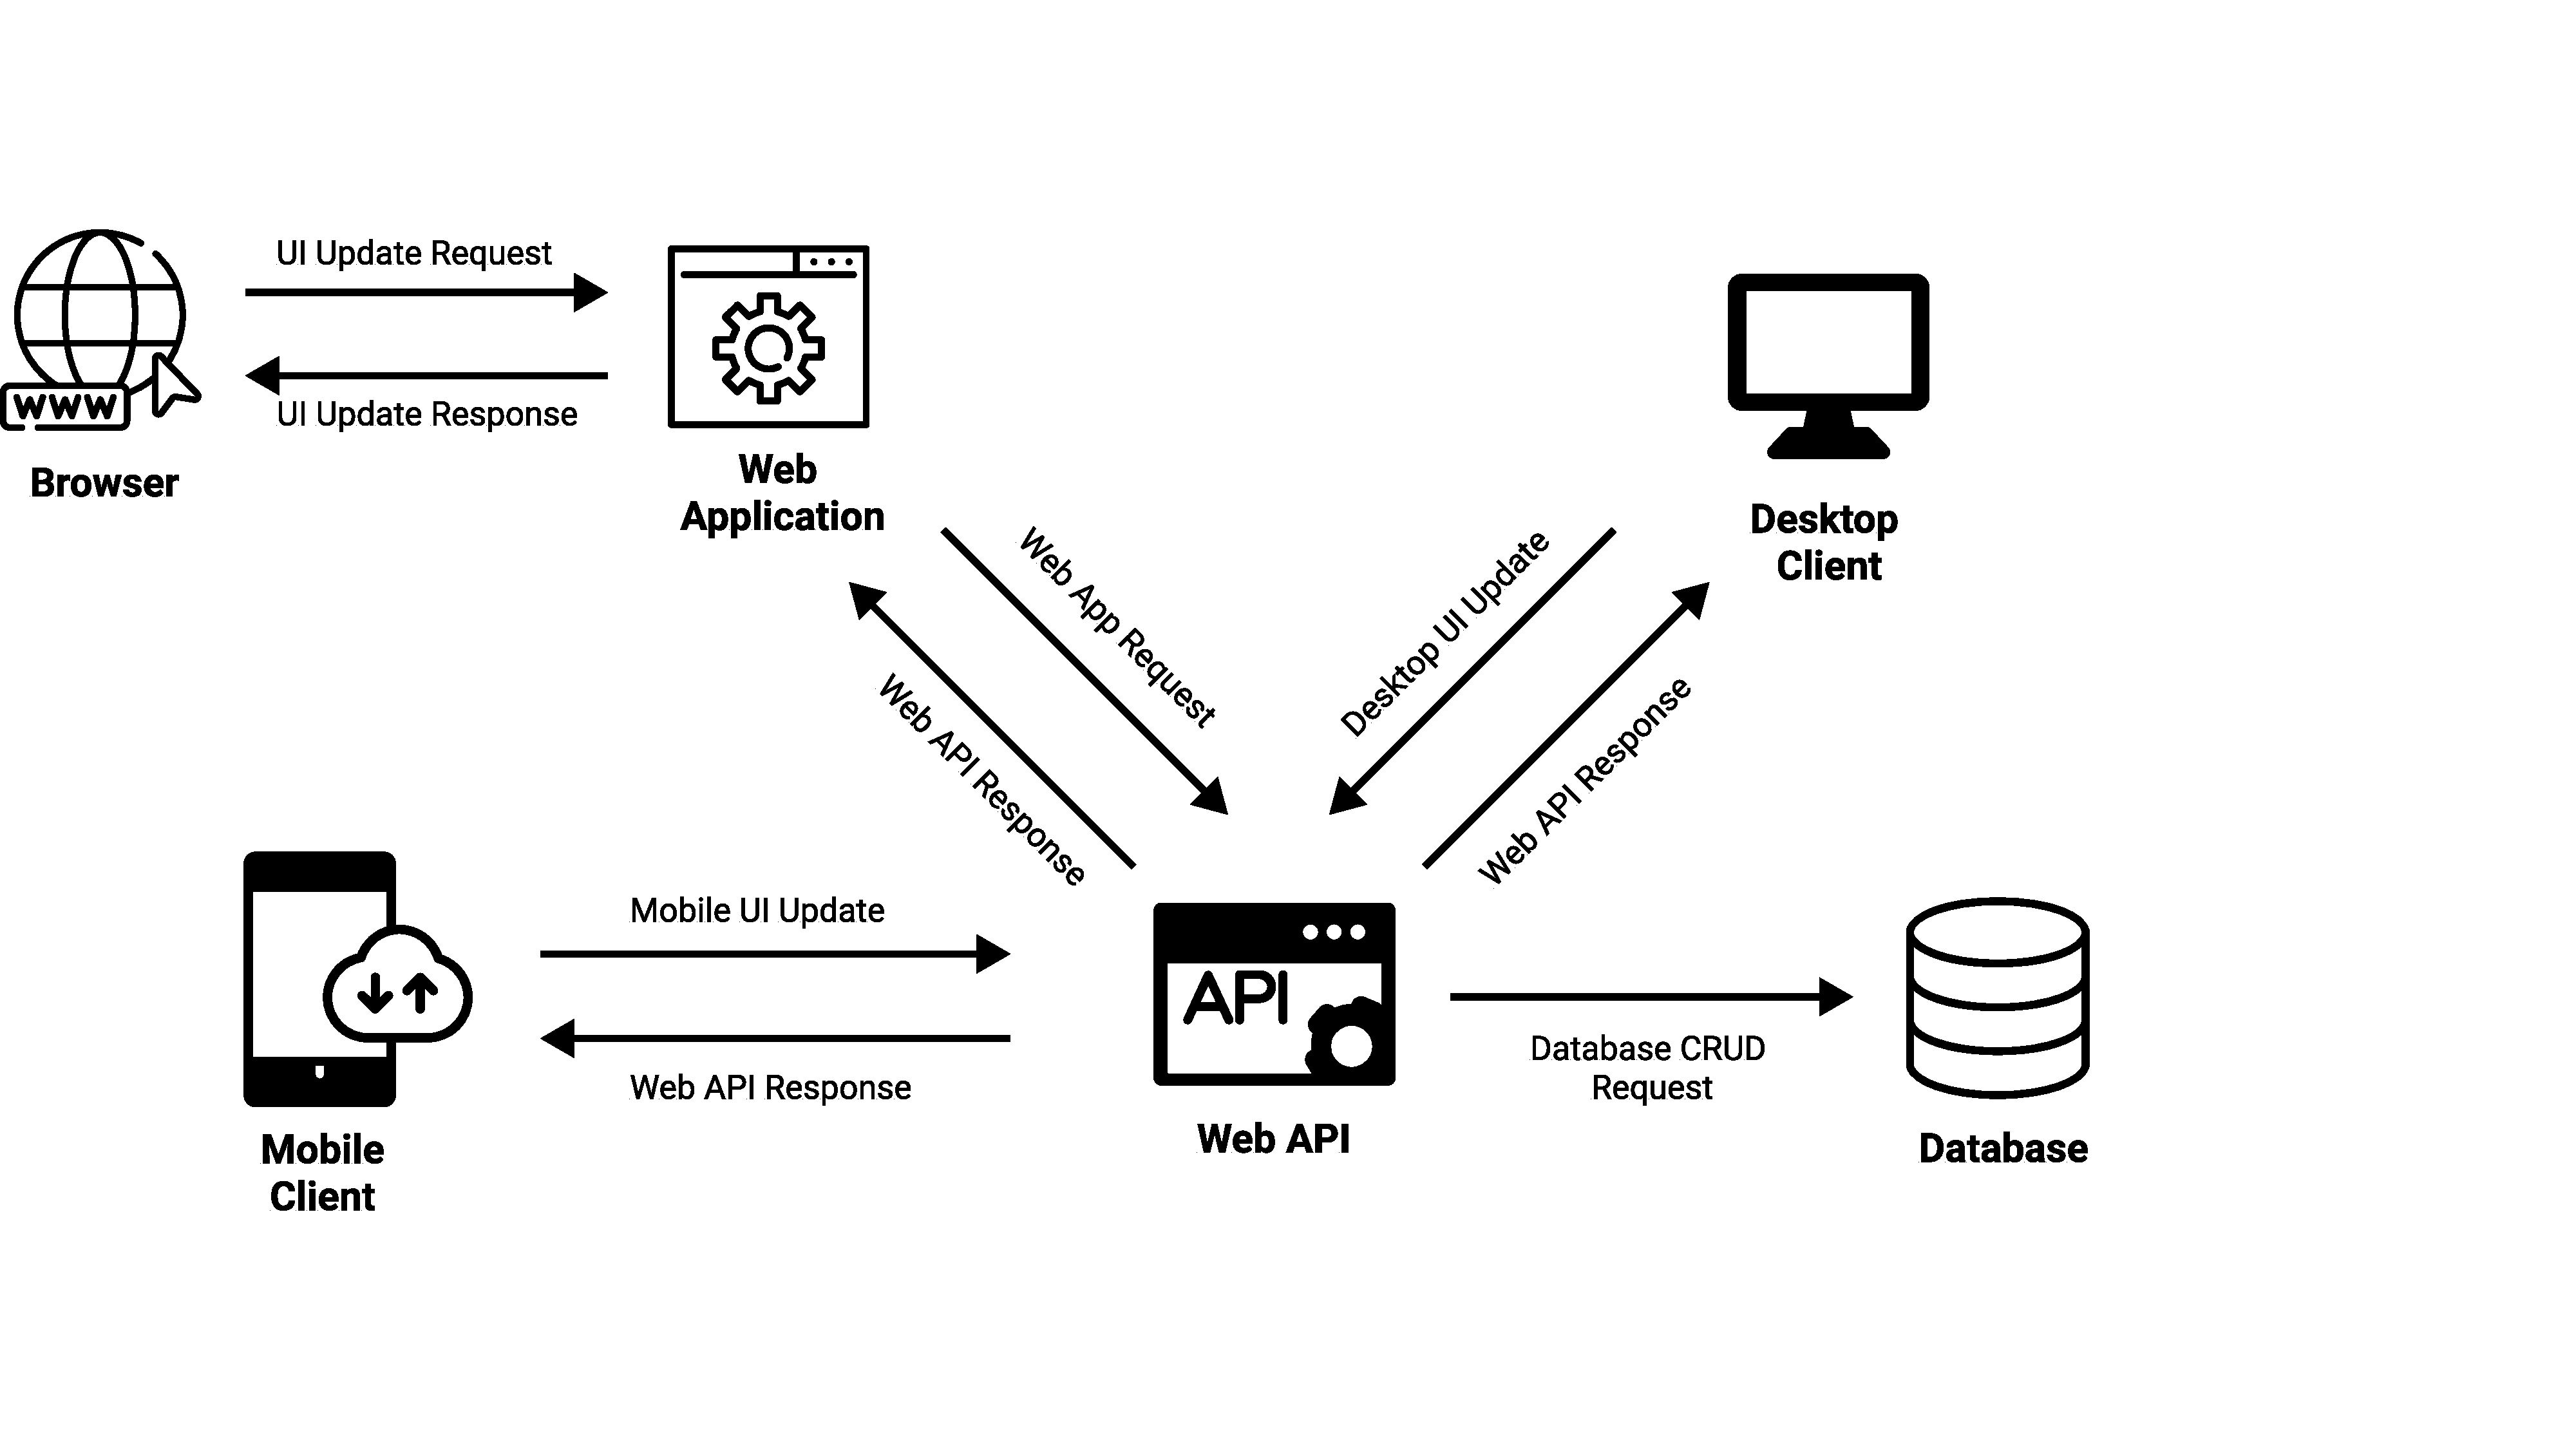
\includegraphics[width=1.2\textwidth]{Pictures/Threat_Modeling}
    \caption{Database diagram.}\label{fig:figure6}
\end{figure}

\begin{enumerate}
    \item \textbf{Browser UI Update Request}
    \begin{itemize}
        \item \textbf{Treat 1.1.} An adversary can perform action on behalf of other user due to lack of controls against cross domain requests.
        \item \textbf{Treat 1.2.} An adversary may bypass critical steps or perform actions on behalf of other users (victims) due to improper validation logic.
        \item \textbf{Treat 1.3.} An adversary can reverse weakly encrypted or hashed content.
        \item \textbf{Treat 1.4.} An adversary may gain access to sensitive data from log files.
        \item \textbf{Treat 1.5.} An adversary can spoof the target web application due to insecure TLS certificate configuration.
        \item \textbf{Treat 1.6.} An adversary can steal sensitive data like user credentials.
        \item \textbf{Treat 1.7.} An adversary can gain access to sensitive data stored in Web App's config files.
        \item \textbf{Treat 1.8.} An adversary can gain access to sensitive data by performing SQL injection through Web App.
        \item \textbf{Treat 1.9.} An attacker steals messages off the network and replays them in order to steal a user's session.
        \item \textbf{Treat 1.10.} An adversary can deface the target web application by injecting malicious code or uploading dangerous files.
        \item \textbf{Treat 1.11.} An adversary may spoof Desktop Web Browser (Chrome) and gain access to Web Application.
        \item \textbf{Treat 1.12.} An adversary can create a fake website and launch phishing attacks.
        \item \textbf{Treat 1.13.} Attackers can steal user session cookies due to insecure cookie attributes.
        \item \textbf{Treat 1.14.} An adversary can get access to a user's session due to insecure coding practices.
        \item \textbf{Treat 1.15.} An adversary can get access to a user's session due to improper logout and timeout.
        \item \textbf{Treat 1.16.} Attacker can deny the malicious act and remove the attack foot prints leading to repudiation issues.
        \item \textbf{Treat 1.17.} An adversary may gain access to sensitive data from uncleared browser cache.
        \item \textbf{Treat 1.18.} An adversary can gain access to sensitive information through error messages.
        \item \textbf{Treat 1.19.} An adversary can gain access to sensitive data by sniffing traffic to Web Application.
        \item \textbf{Treat 1.20.} An adversary can gain access to certain pages or the site as a whole.
        \item \textbf{Treat 1.21.} An adversary may gain access to unmasked sensitive data such as credit card numbers.
    \end{itemize}
    \item \textbf{Web App Request}
    \begin{itemize}
        \item \textbf{Treat 2.1.} An adversary may gain unauthorized access to Web API due to poor access control checks.
        \item \textbf{Treat 2.2.} An adversary can gain access to sensitive information from an API through error messages.
        \item \textbf{Treat 2.3.} An adversary can gain access to sensitive data by sniffing traffic to Web API\@.
        \item \textbf{Treat 2.4.} An adversary can gain access to sensitive data stored in Web API's config files.
        \item \textbf{Treat 2.5.} Attacker can deny a malicious act on an API leading to repudiation issues.
        \item \textbf{Treat 2.6.} An adversary may spoof Mango Web Application and gain access to Web API\@.
        \item \textbf{Treat 2.7.} An adversary may inject malicious inputs into an API and affect downstream processes.
        \item \textbf{Treat 2.8.} An adversary can gain access to sensitive data by performing SQL injection through Web API\@.
    \end{itemize}
    \item \textbf{Web API Response}
    \begin{itemize}
        \item \textbf{Treat 3.1.} An adversary can reverse weakly encrypted or hashed content.
        \item \textbf{Treat 3.2.} An adversary may gain access to sensitive data from log files.
        \item \textbf{Treat 3.3.} An adversary can gain access to sensitive information through error messages.
        \item \textbf{Treat 3.4.} Attacker can deny the malicious act and remove the attack foot prints leading to repudiation issues.
        \item \textbf{Treat 3.5.} An adversary can spoof the target web application due to insecure TLS certificate configuration.
        \item \textbf{Treat 3.6.} An adversary can steal sensitive data like user credentials.
        \item \textbf{Treat 3.7.} An adversary can create a fake website and launch phishing attacks.
    \end{itemize}
    \item \textbf{CRUD Request}
    \begin{itemize}
        \item \textbf{Treat 4.1.} An adversary can gain unauthorized access to database due to loose authorization rules.
        \item \textbf{Treat 4.2.} An adversary can gain access to sensitive PII or HBI data in database.
        \item \textbf{Treat 4.3.} An adversary can gain access to sensitive data by performing SQL injection.
        \item \textbf{Treat 4.4.} An adversary can deny actions on database due to lack of auditing.
        \item \textbf{Treat 4.5.} An adversary can tamper critical database securables and deny the action.
        \item \textbf{Treat 4.6.} An adversary may leverage the lack of monitoring systems and trigger anomalous traffic to database.
        \item \textbf{Treat 4.7.} An adversary can gain unauthorized access to database due to lack of network access protection.
    \end{itemize}
    \item \textbf{Mobile UI Update}
    \begin{itemize}
        \item \textbf{Treat 5.1.} An adversary can gain access to sensitive data by performing SQL injection through Web API.
        \item \textbf{Treat 5.2.} An adversary can reverse engineer and tamper binaries.
        \item \textbf{Treat 5.3.} An adversary may inject malicious inputs into an API and affect downstream processes.
        \item \textbf{Treat 5.4.} An adversary may spoof Mobile App (IOS, Android) and gain access to Web API\@.
        \item \textbf{Treat 5.5.} An adversary obtains refresh or access tokens from Mobile App (IOS, Android) and uses them to
        obtain access to the Mango Web API\@.
        \item \textbf{Treat 5.6.} Attacker can deny a malicious act on an API leading to repudiation issues.
        \item \textbf{Treat 5.7.} An adversary can gain access to sensitive data stored in Web API's config files.
        \item \textbf{Treat 5.8.} An adversary can gain sensitive data from mobile device.
        \item \textbf{Treat 5.9.} An adversary can gain access to sensitive data by sniffing traffic to Web API\@.
        \item \textbf{Treat 5.10.} An adversary can gain access to sensitive data by sniffing traffic from Mobile client.
        \item \textbf{Treat 5.11.} An adversary can gain access to sensitive information from an API through error messages.
        \item \textbf{Treat 5.12.} An adversary may gain unauthorized access to Web API due to poor access control checks.
        \item \textbf{Treat 5.13.} An adversary may jail break into a mobile device and gain elevated privilege.
    \end{itemize}
\end{enumerate}

\subsection*{4. System Requirements}\label{subsec:system-requirements}
Prior to software module implementation, it is essentially important to define the functionality module will obtain.
In this section we discuss functional and non-functional requirements of secure instant messaging system from customer's prospective.
Generally, there are three forms of software product requirements: business, functional, and non-functional.
Business requirements [\cite{dilworth2007creation}] typically answer how the product will address the needs of your company and its users.
They also reveal the business model of the app and what problems it can solve.
Functional requirements [\cite{malan2001functional}] are about functionalities that will be implemented in the application.
Non-functional requirements [\cite{chung2012non}] describe how these functionalities will be implemented.

\input{Files/functional-requirements.tex}

\subsection*{5. Web service architecture}\label{subsec:web-service-architecture}
\textbf{Motivation.} Implementing the instant messenger system, we consider applying a well-known N-tier
Monolithic Architecture [\cite{bucchiarone2018monolithic}], which provides a time-proven model that allows software
developers to create flexible and reusable applications.

However, during the implementation of monolith it is very important to avoid the cases of crucial over-engineering
of the system that leads to useless complication of the code base.
For the developers, it is a vital point to follow the KISS [\cite{alwin2016kiss}] and YAGNI [\cite{da2018evolution}]
software development principles in order not to reach
\href{https://github.com/smartstore/SmartStoreNET/blob/4.x/src/Presentation/SmartStore.Web/Controllers/CatalogHelper.cs}
{thousands lines}
of code in a single class.

One would suggest to use nowadays popular Microservices Architecture, thinking about scalability [\cite{brataas2004exploring}],
an ability of the system to handle large numbers of users distributed over geographically large areas without
notably affecting the overall performance of the system.
However, the effect of Microservices is being felt only for quite large and complex systems,
not the case of our yet simple application.
According to \href{https://martinfowler.com/bliki/MonolithFirst.html}{Martin Fowler},
\begin{quote}
    \textit{you shouldn't start a new project with microservices, even if you're sure your application will be big enough to
    make it worthwhile.}
\end{quote}
which is so-called \textit{Monolith first} approach.
Makes sense to begin an implementation from \textit{Modular monolith}, a monolith with minimized coupling between the
software components, where splitting to microservice won't be a time and financial expensive operation.
Following plot demonstrates the relation between the complexity and profits between monolith and microservices

\begin{figure}[H]
    \centering
    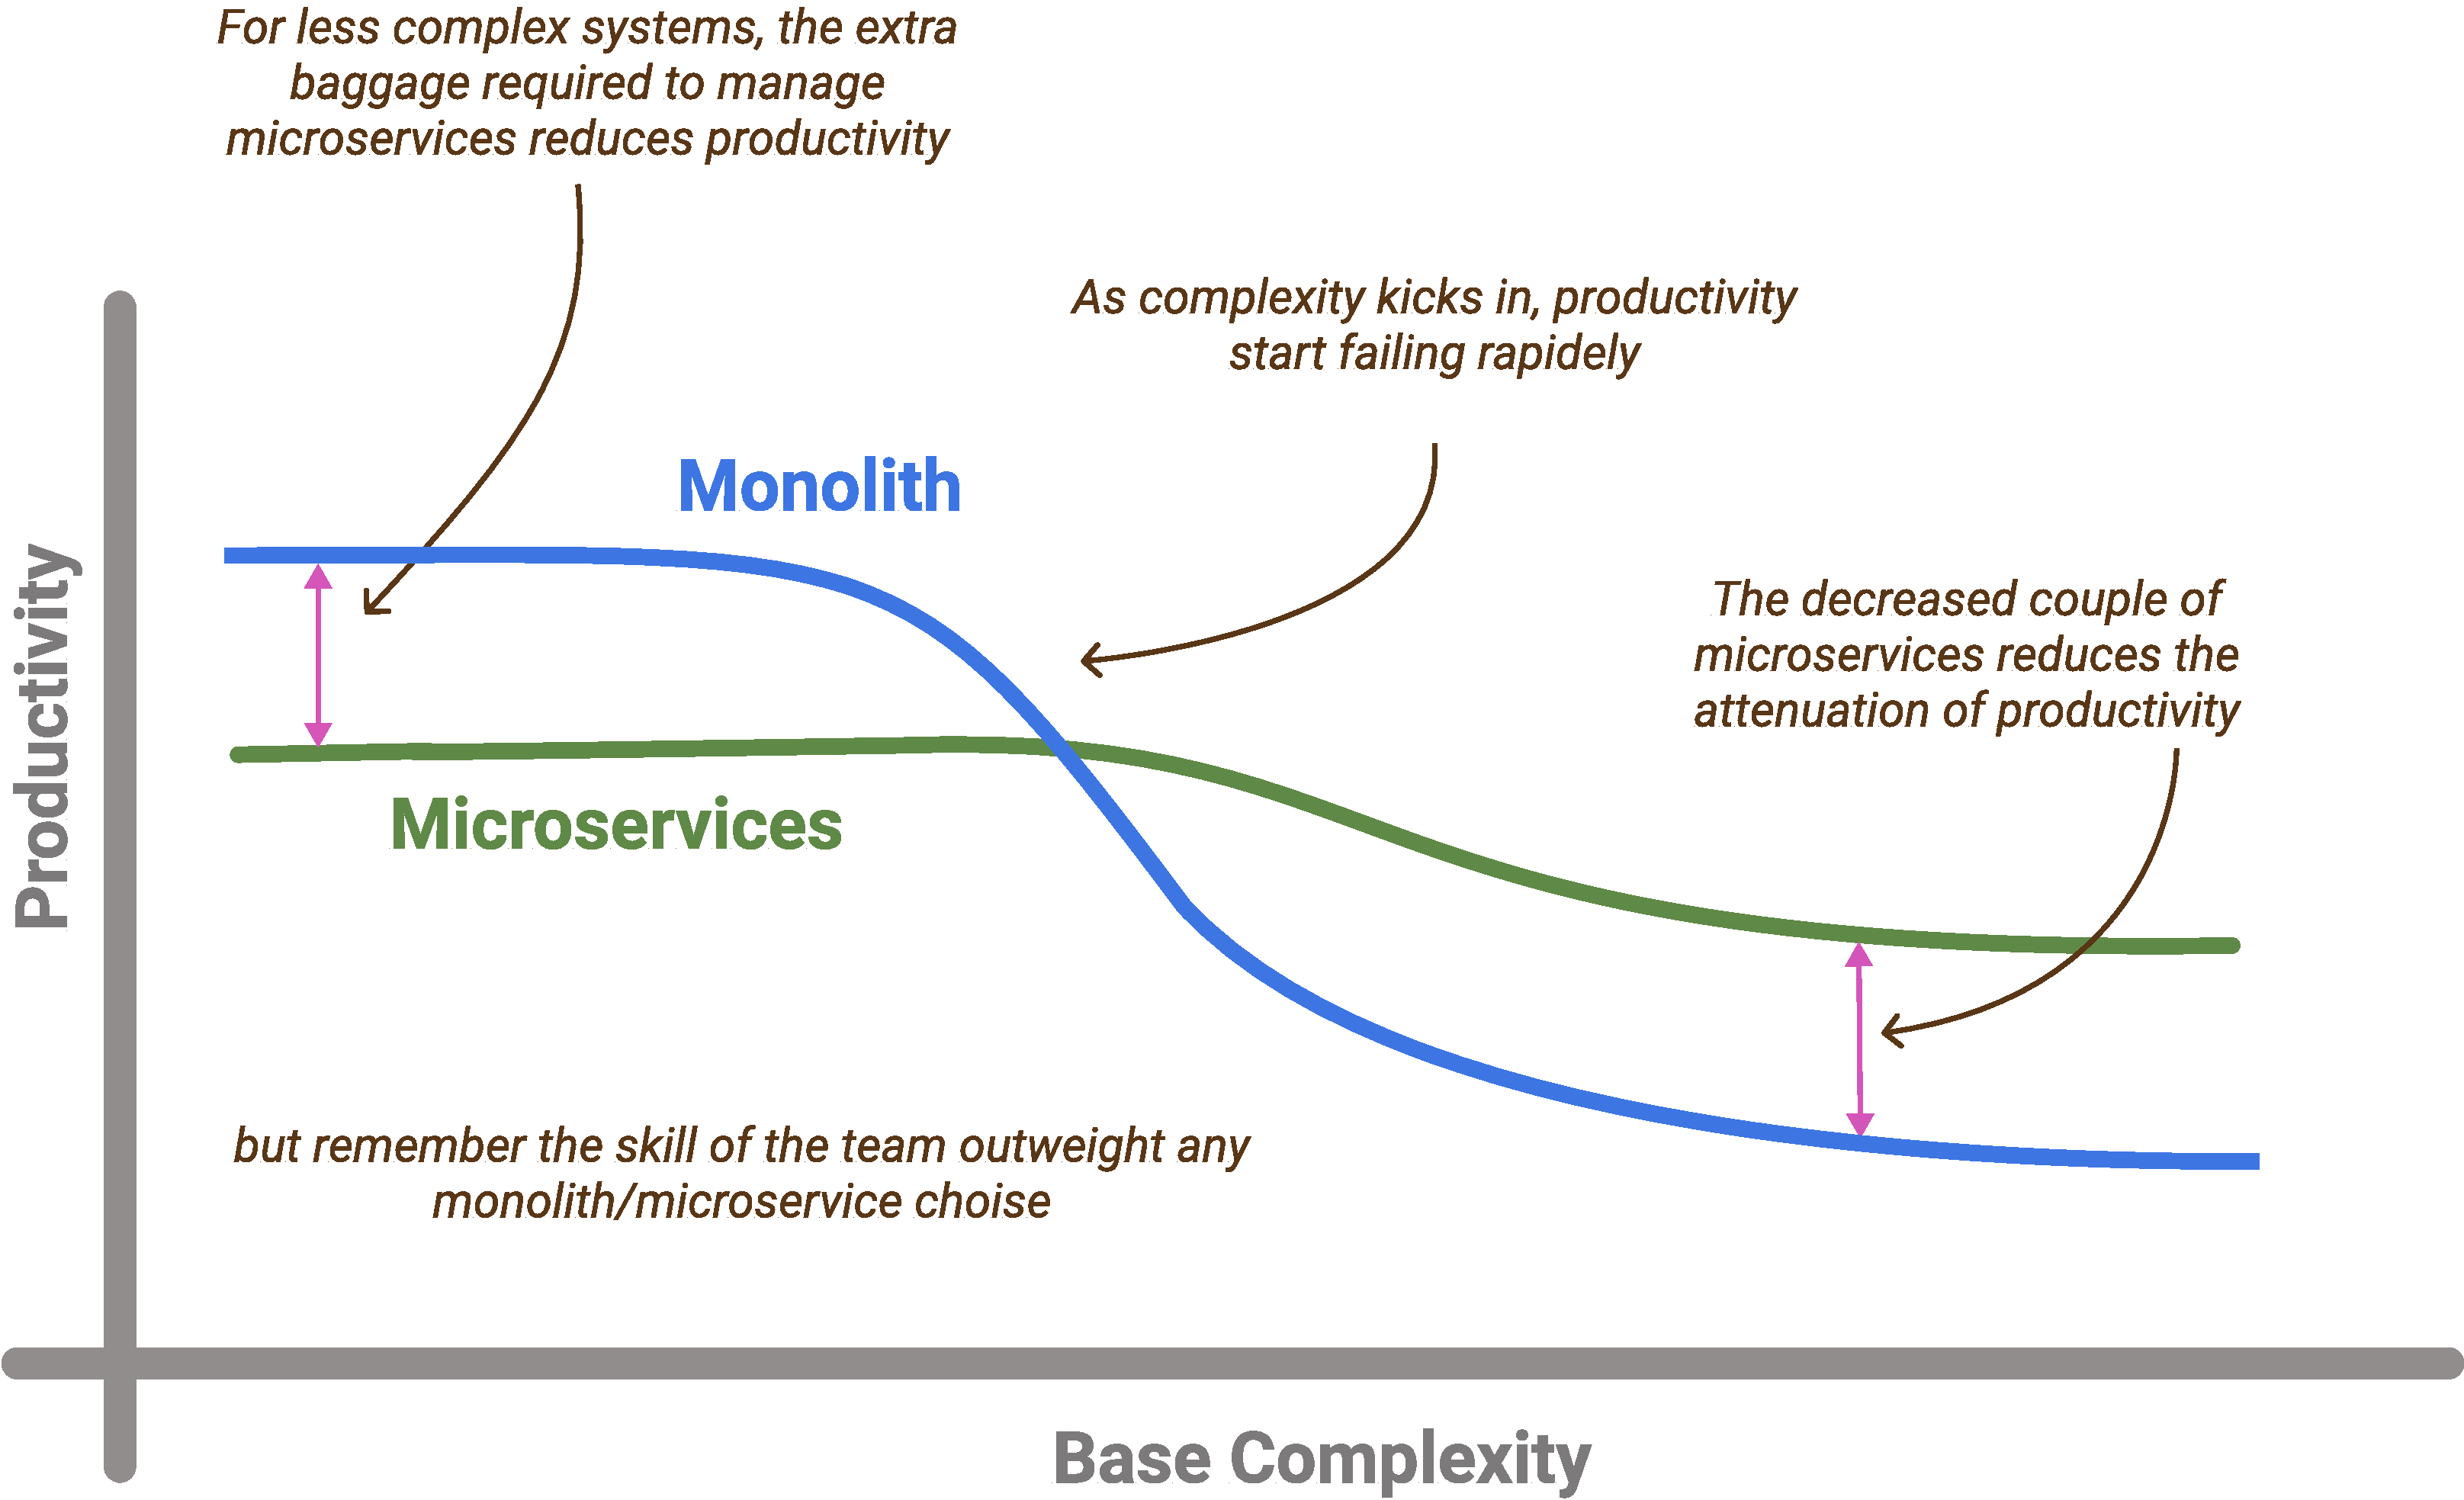
\includegraphics[width=1\textwidth]{Pictures/02_Monolith_and_Microservices_complexity}
    \caption{Relation between system complexity and architectures.
    Source: \href{https://martinfowler.com/bliki/MicroservicePremium.html}{Martin Fowler.}}
    \label{fig:monolith_vs_microservice}
\end{figure}

A layered architecture usually consists of Presentation layer, Business logic layer, Data access layer.
By segregating the project into layers, developers reach the options to modify or add a specific layer
without reworking the entire application.

\begin{itemize}
    \item \textit{Presentation Layer.} Graphic user interface or API gateway.
    \item \textit{Application Logic.} Encapsulates the means of interaction with user.
    For example, push-notifications e-mail notification, sms notifications etc.
    \item \textit{Business Logic.} Encapsulates the logic of clint's request handling.
    For example, service layer.
    \item \textit{Data Access Layer.} Responsible for logging, database access and other services required to support
    Business Logic layer.
\end{itemize}

\begin{figure}[H]
    \centering
    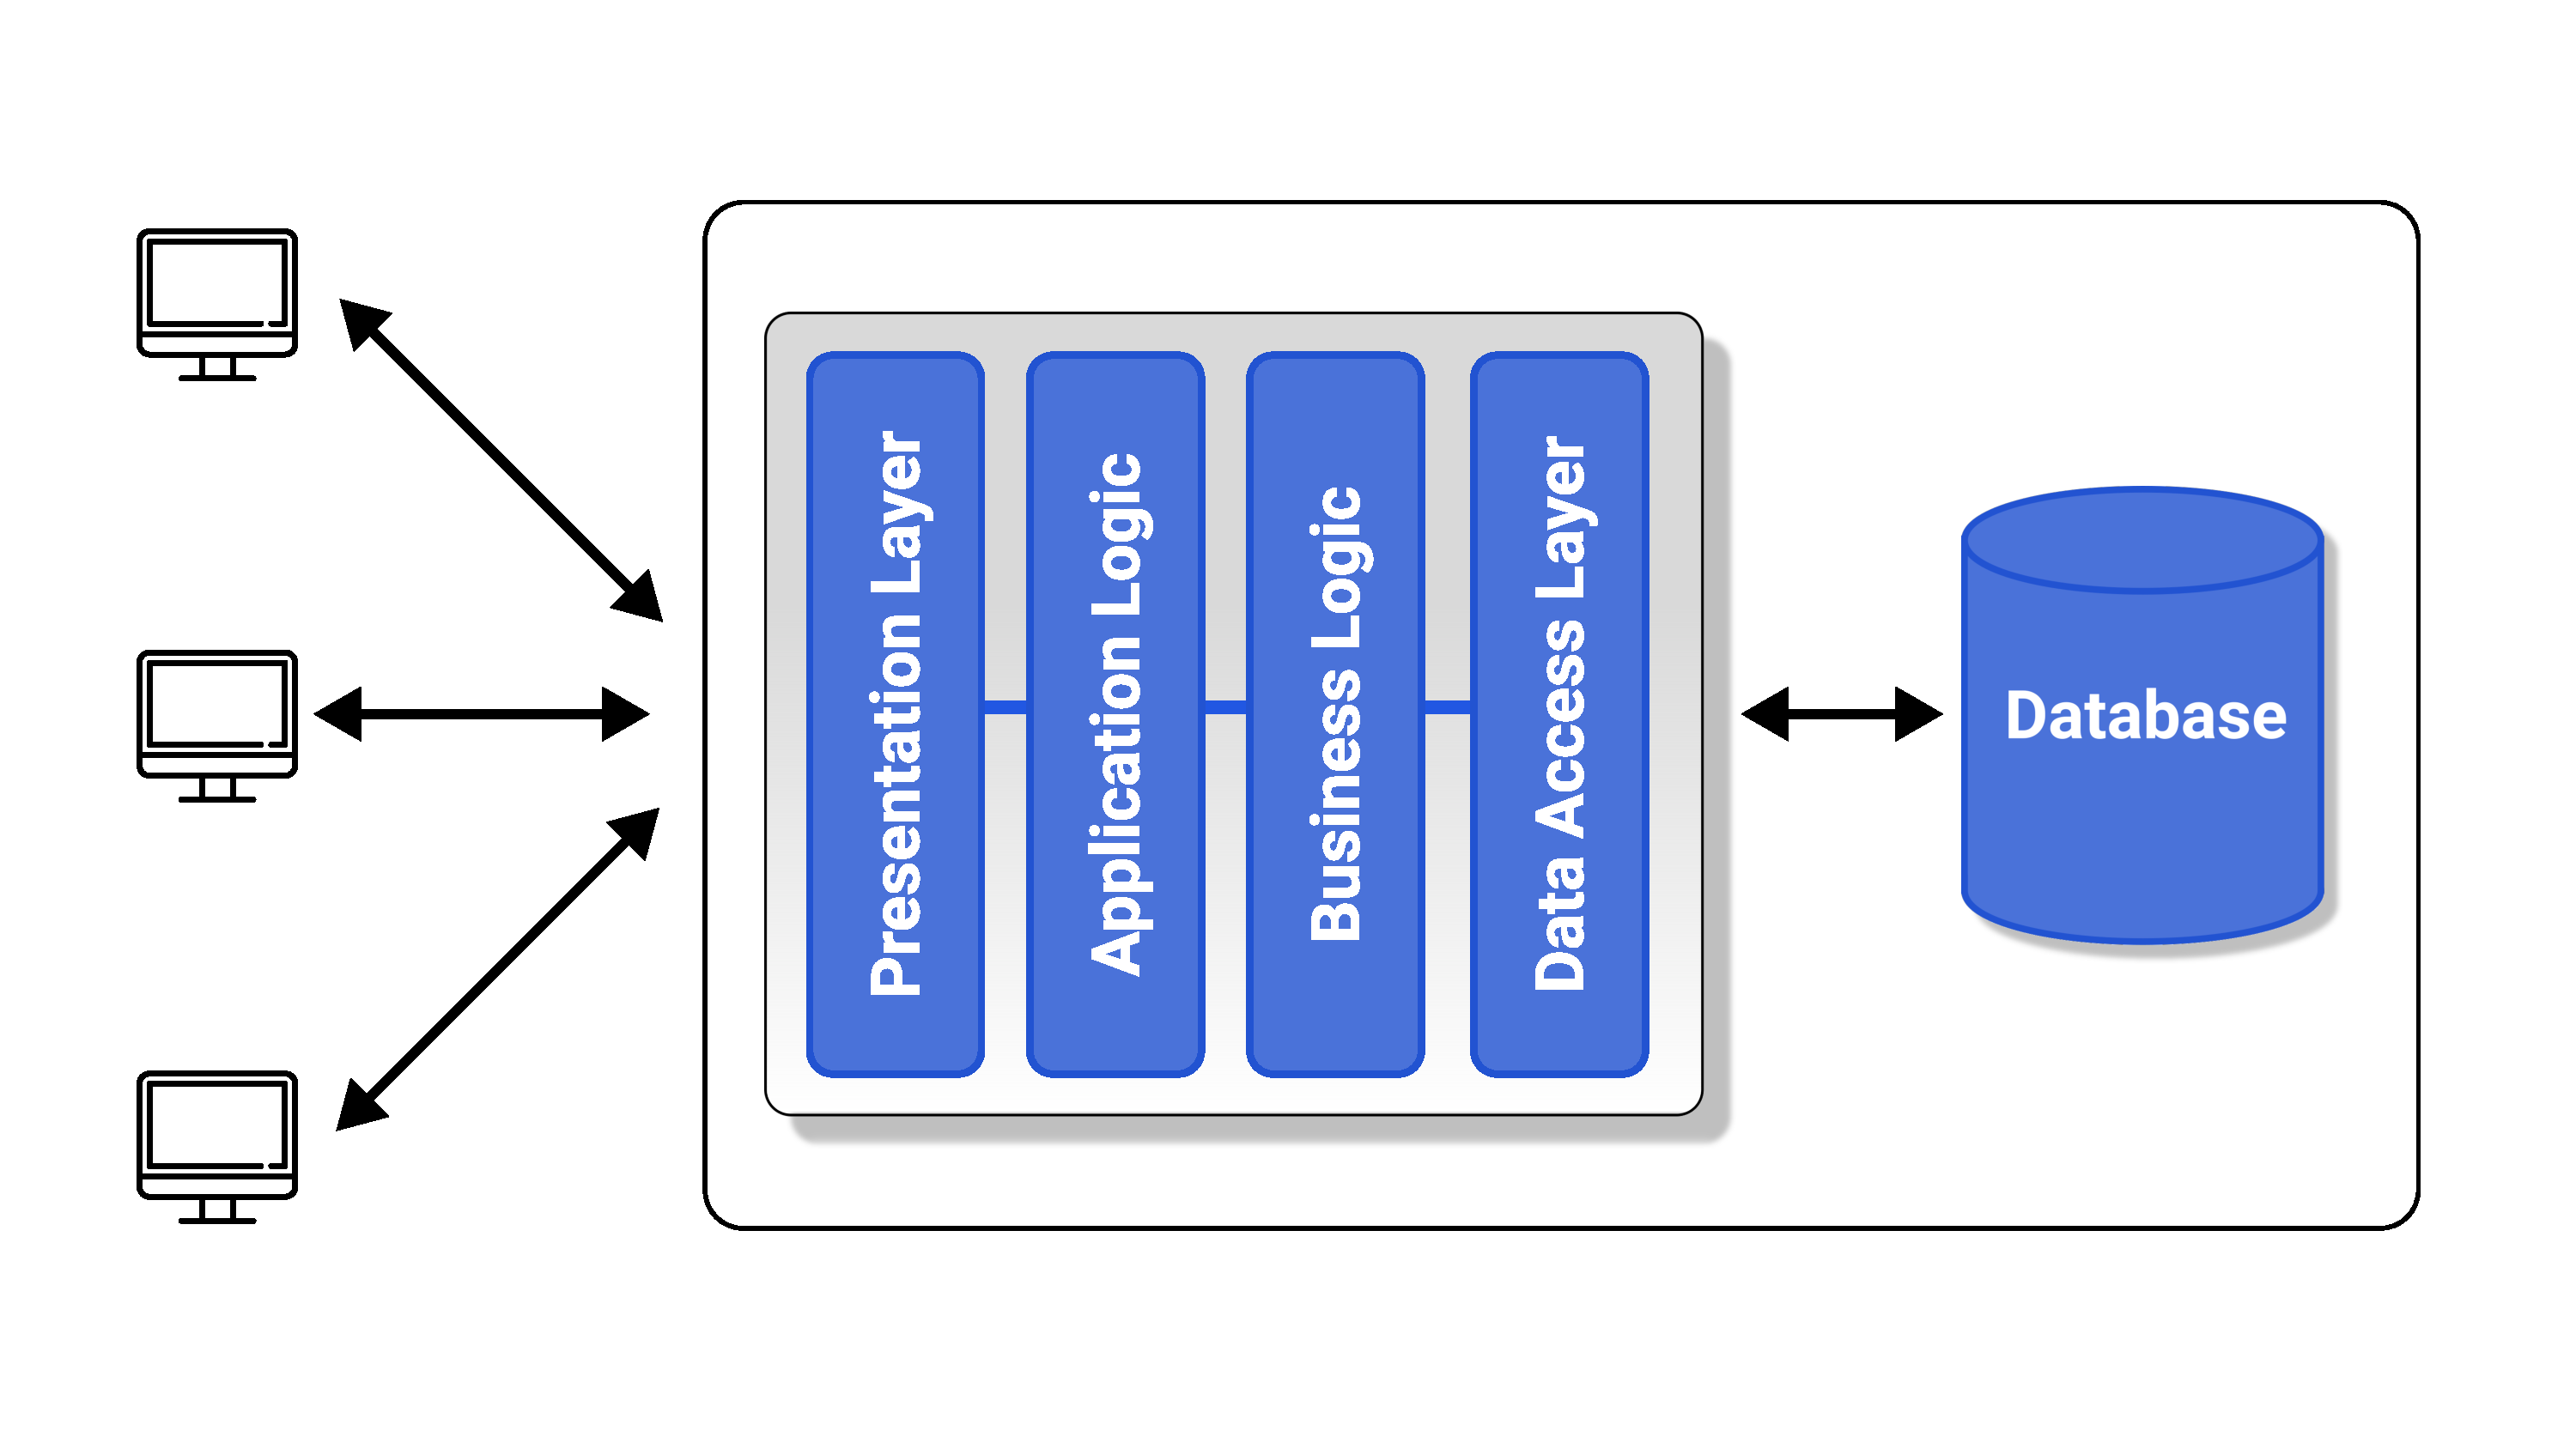
\includegraphics[width=1\textwidth]{Pictures/03_Monolith_concept_diagram}
    \caption{Monolith concept diagram.}\label{fig:figure2}
\end{figure}

\textbf{Monolithic Architecture: Cons and Props.} A monolith is built as a large system with a single code base and
deployed as a single unit, usually behind a load balancer.
Monoliths offer several advantages, particularly when it comes to operational overhead requirements.
Here are some of those basic benefits:

\begin{itemize}
    \item \textit{Simplicity.} Monolithic architectures are simple to build and deploy.
    These applications can scale horizontally, by running several copies of the application behind a load balancer.
    With a single codebase, monolithic apps can easily handle cross-cutting concerns, such as logging,
    configuration management and performance monitoring.
    Another advantage associated with the simplicity of monolithic applications is easier deployment.
    When it comes to monolithic applications, you do not have to handle many deployments but just one.
    \item \textit{Performance.} Components in a monolith typically share memory which is faster than service-to-service
    communications using IPC [\cite{proctor1999linux}] or other mechanisms.
    \item \textit{Easier debugging and testing.}
    In contrast to the microservices, monolithic applications are much easier to debug and test.
    Since that monolithic application is a single indivisible unit the process of end-to-end testing is much faster.
    \item \textit{Easier development.} As long as the monolithic approach is a standard way of building applications,
    any engineering team has the right knowledge and capabilities to develop a monolithic application.
\end{itemize}

However, the drawback of monolithic architectures hides in their tight coupling.
Over time, monolithic components and layers become tightly coupled and entangled, effecting management, scalability
and continuous deployment.
Another disadvantages of the monoliths include:
\begin{itemize}
    \item \textit{Understanding.} When a monolithic application's code base grows up, it becomes too complicated to understand.
    Obviously, huge code base of monolithic app is hard to manage therefore.
    \item \textit{Reliability.} Entire application down may be caused by an error in every single component.
    \item \textit{Updates.} Single and large code base causes the needs to redeploy an application on every single update.
    \item \textit{Technology stack.} Technology stack of the monolithic app is limited by the technologies and providers
    used from the beginning of development.
    It makes technology stack changes to be expensive in terms of finances and time.
    \item \textit{Scalability.} Application's components cannot be scaled independently, an entire application should be scaled.
\end{itemize}

\textbf{Minimization of services coupling.} As we see, the monolith has its own disadvantages, like for instance:
understanding the project structure, reliability concerns, technology stack limitations, scalability limitations.
Obviously, some of these disadvantages cannot be mitigated because of the nature of the monolith.
However, the complexity and coupling problem can be minimized applying certain approaches.
Frequent violation of the single-responsibility principle of SOLID during implementing service components
in business logics layer causes the over-complication of codebase over the time.
The reason is that service components keep the huge number of methods in order to handle all possible CRUD requests
to the database without any bounded context.
Although, the SOLID rules are very powerful in solving designated code issues, it is necessary to apply them very carefully,
since that most of them require high level of abstractions, which increases in size the code base and complicates the
solution.
Do not overcomplicate the solution without any reason following \textit{Open-Closed Principle}.
Schematically, the service entity is as follows
\begin{figure}[H]
    \centering
    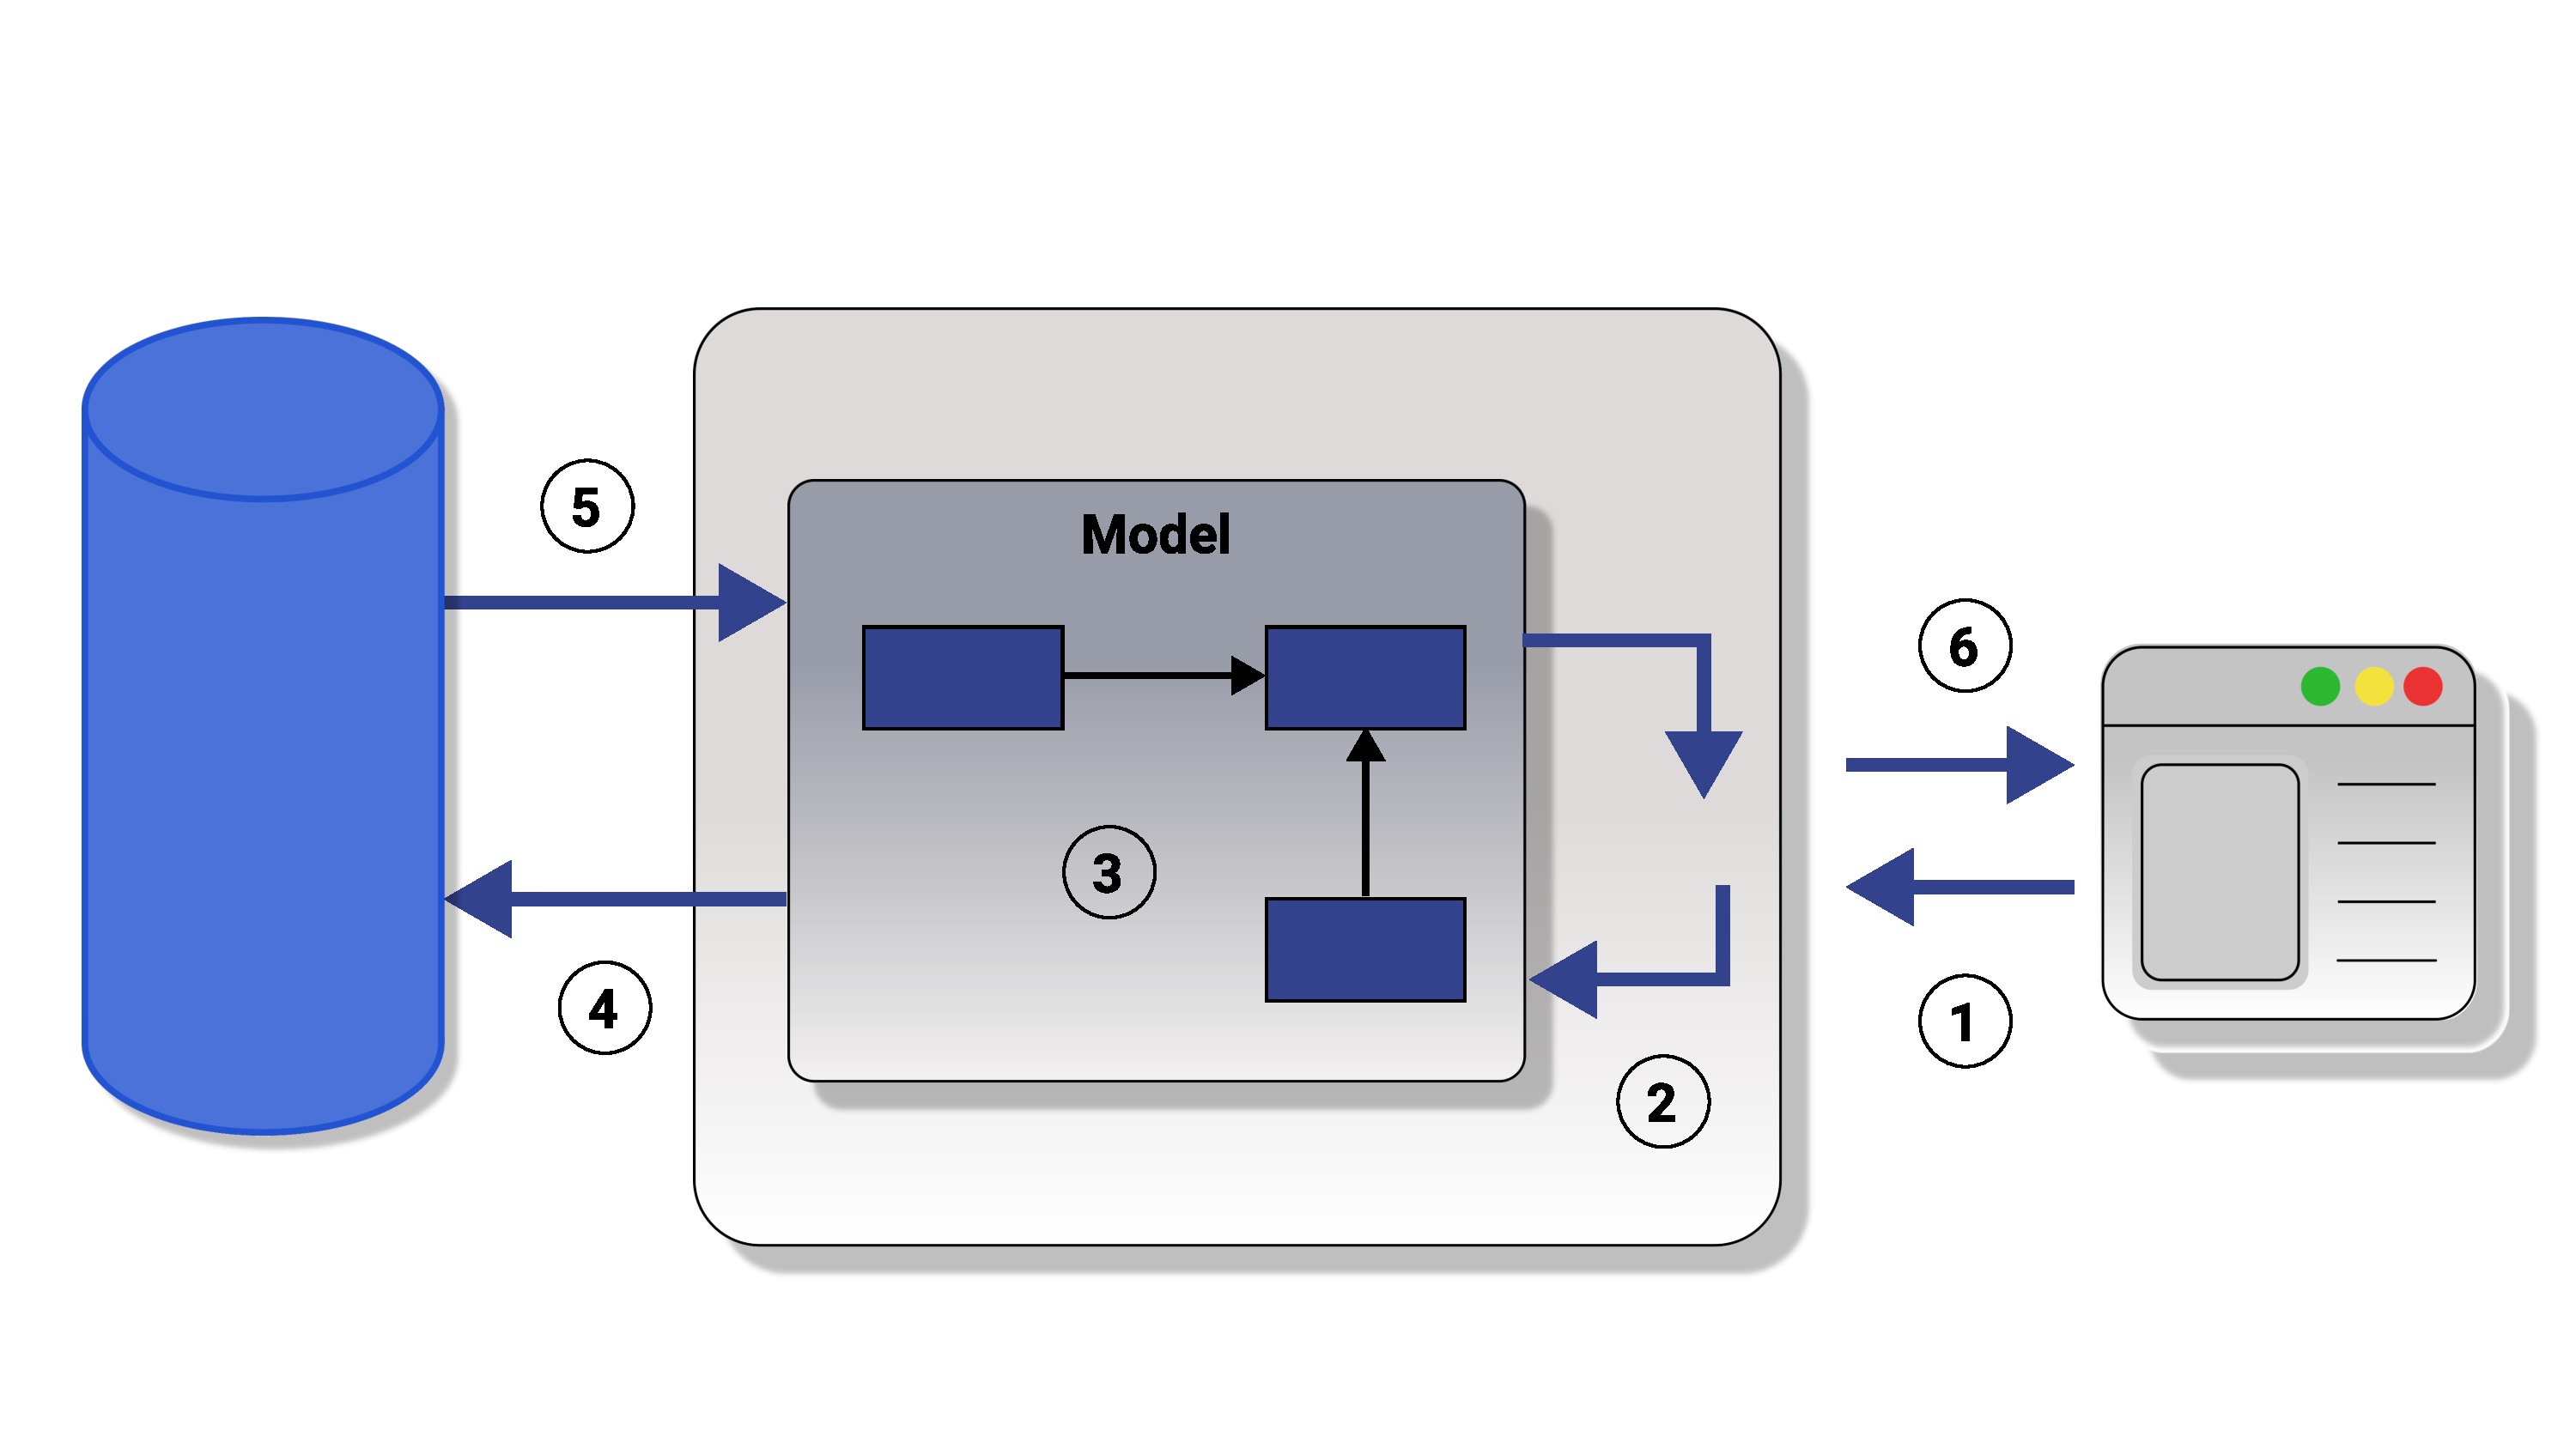
\includegraphics[width=1\textwidth]{Pictures/04_Service_entity_concept_diagram}
    \caption{Service entity concept diagram.
    Source: \href{https://martinfowler.com/bliki/CQRS.html}{Martin Fowler}.}\label{fig:figure9}
\end{figure}
Where the steps are
\begin{enumerate}
    \item User makes a change in UI\@.
    \item Change forwarded to model.
    \item Model executes validation and business logic.
    \item Model updates the database.
    \item Model reads from database.
    \item Service updates presentation from query model.
\end{enumerate}

To minimize the natural disadvantages of the monolithic architecture like complexity and high tight coupling of the components
we have to recall the design patterns [\cite{rising1998design}].
In particular, the mediator pattern helps to decouple the components.
Mediator -- is a behavioral design pattern [\cite{rasche2016building}] that allows the communication between two entities,
such that entities doesn't know each other.
Therefore, the program components depend only on a single mediator instance instead of being coupled to multiple of their
colleagues.
In context of .NET platform there are many implementations of the Mediator, the most widely known and used is the
\href{https://github.com/jbogard/MediatR}{MediatR}, which we use in our project.

Another mindset we are going to use in order to minimize complexity and coupling of monolith is Command-Query
Responsibility Segregation (CQRS) principle.
In brief, it stands that read (query) and write (command) requests should be segregated by their responsibilities.
Using CQRS and Mediator together greatly simplifies the project structure and minimizes coupling between business
logic layer components.
CQRS is a pattern that first described by Greg Young [\cite{young2010cqrs}] and its conceptual diagram as follows

\begin{figure}[H]
    \centering
    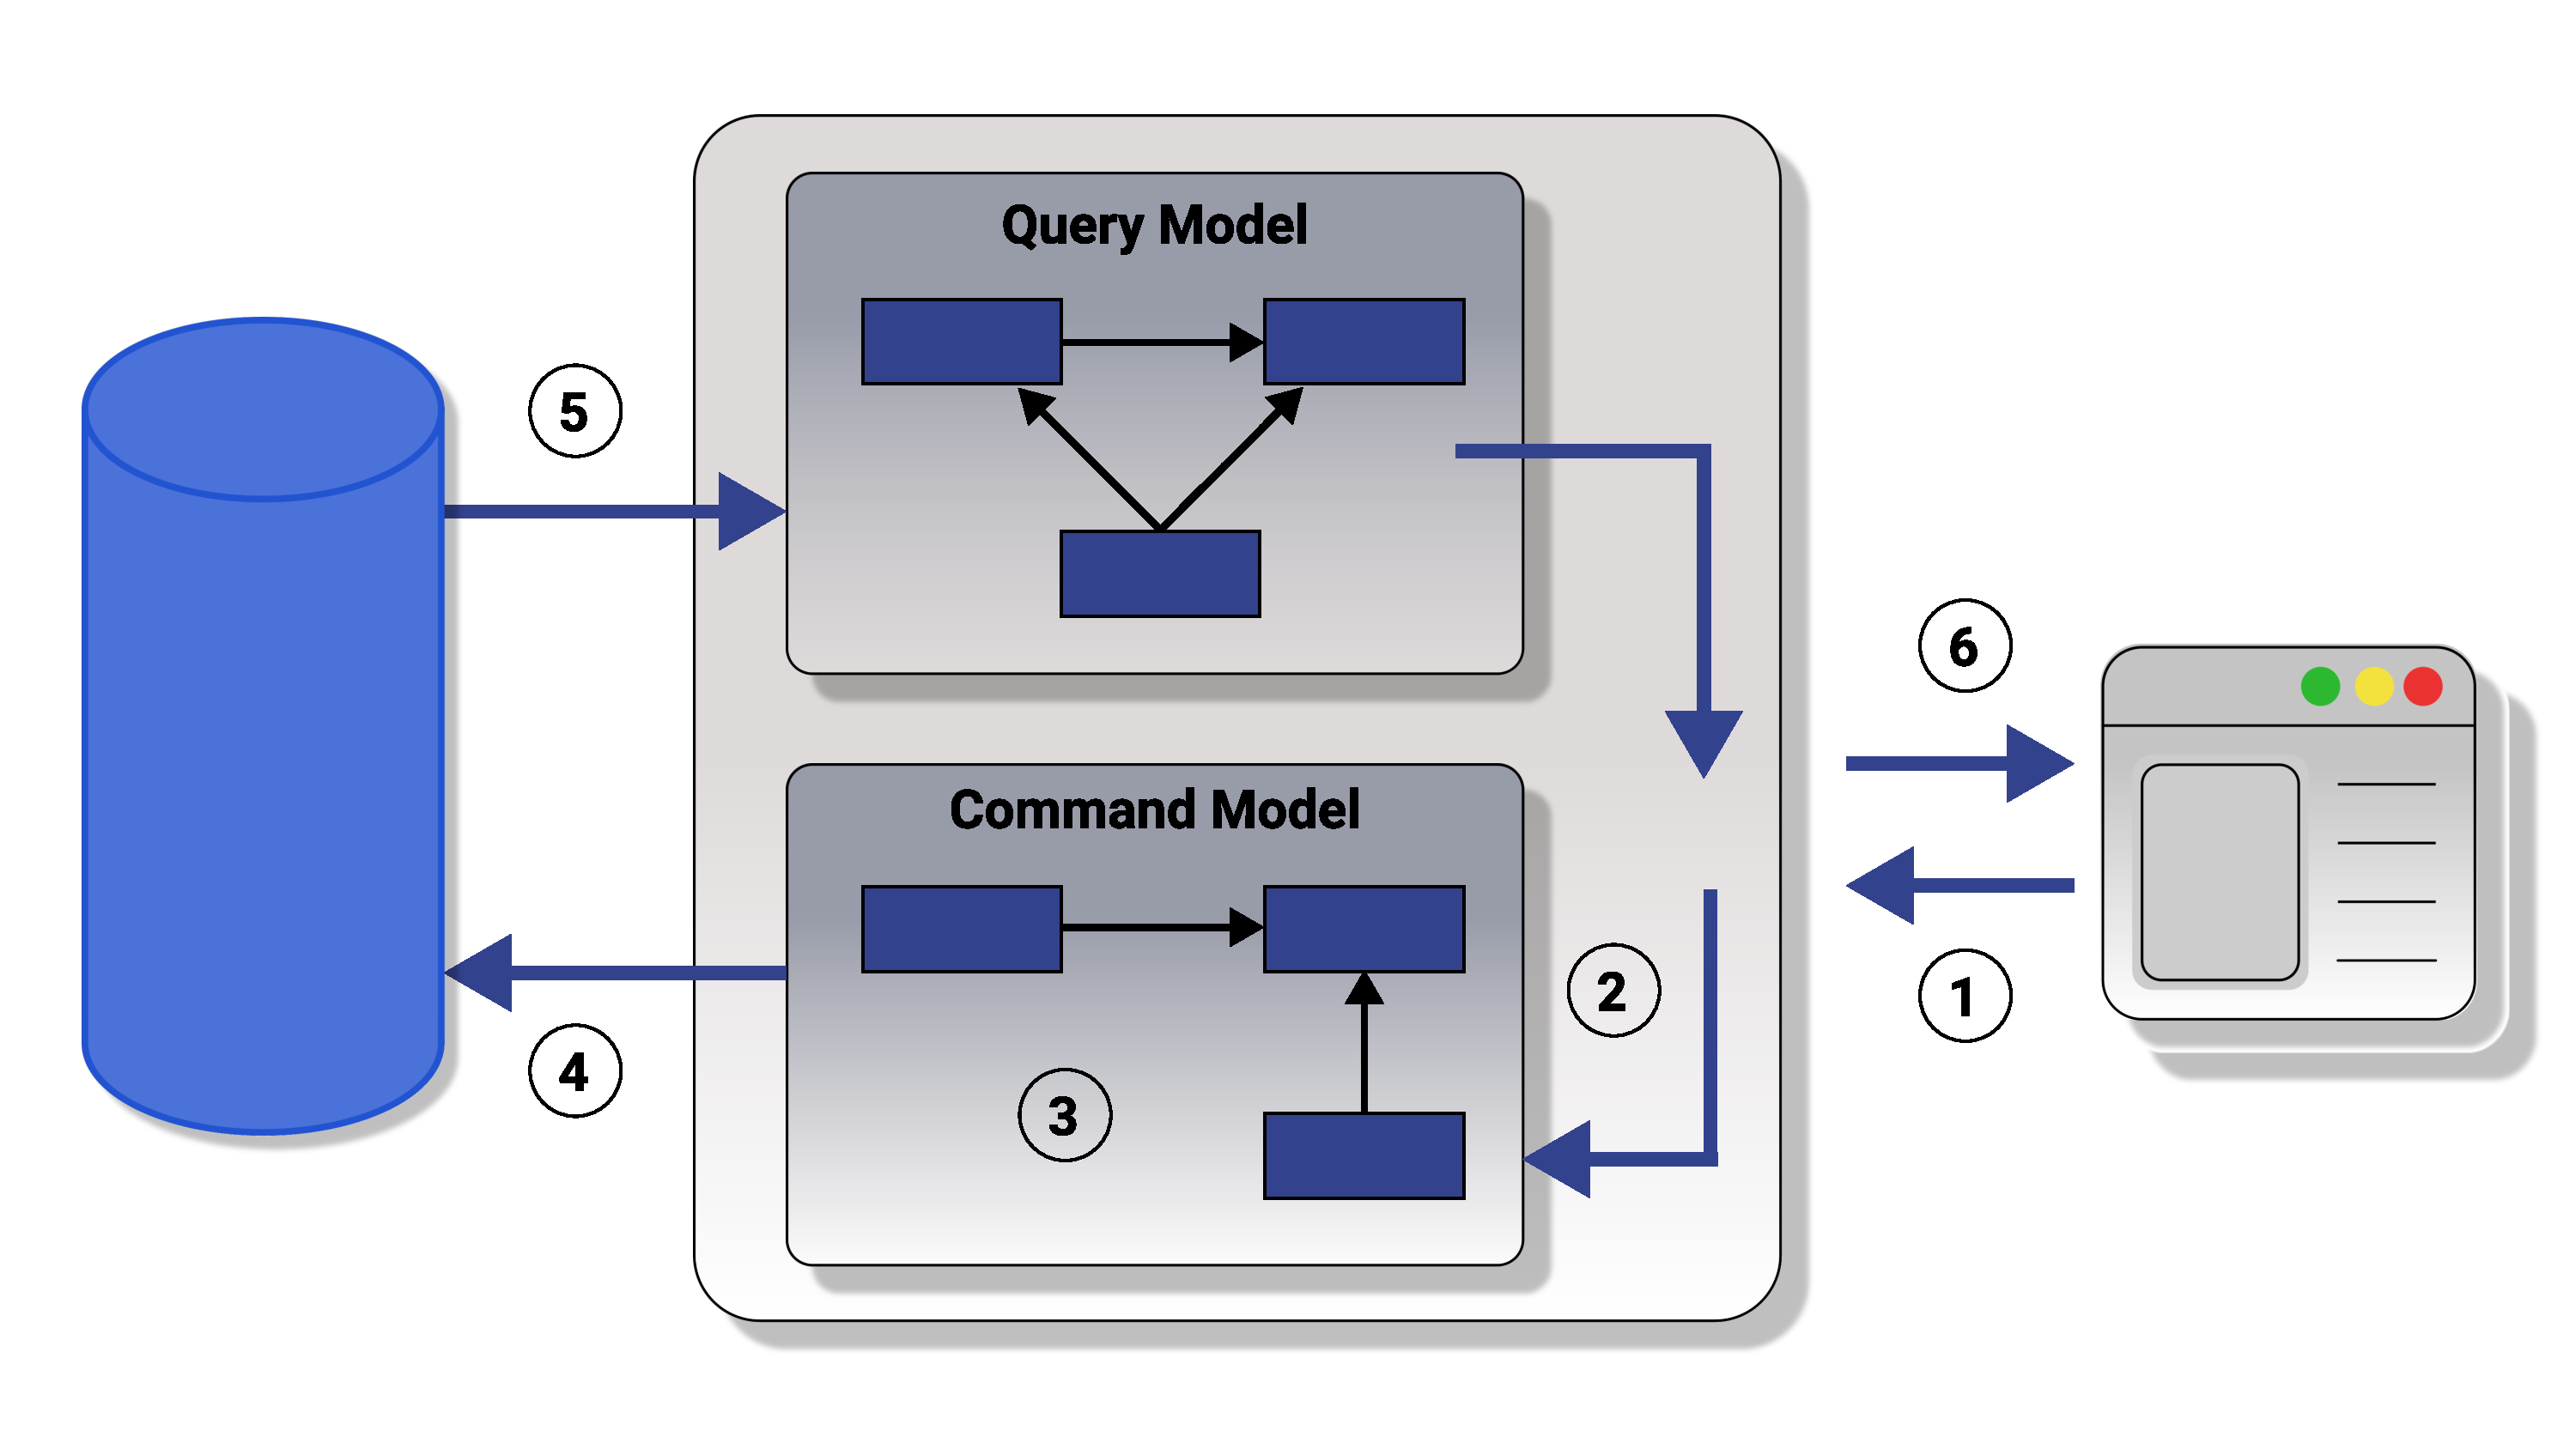
\includegraphics[width=1\textwidth]{Pictures/05_CQRS_concept_diagram}
    \caption{CQRS concept diagram.
    Source: \href{https://martinfowler.com/bliki/CQRS.html}{Martin Fowler}.}
    \label{fig:figure}
\end{figure}

\begin{enumerate}
    \item User makes a change in UI\@.
    \item Application routes information to command model.
    \item Command model executes validation and business logic.
    \item Command model updates the database.
    \item Query model reads from database.
    \item Query service update presentation from query model.
\end{enumerate}

\subsection*{6. Authorization mechanism}\label{subsec:authorization-mechanism}
\textbf{Motivation.} In this section we describe the processes of Authentication and Authorization in the system.
It is worth to remember the meaning of Authentication and Authorization definitions.
Authentication -- is the process of ascertaining that somebody really is who they claim to be [\cite{burrows1989logic}].
Authorization refers to rules that determine who is allowed to do what [\cite{fagin1978authorization}].
For example, Adam may be authorized to create and delete databases, while Catherine is only authorized to read.
The two concepts are completely orthogonal and independent, but both are central to security design, and the
failure to get either one correct opens up the avenue to compromise.
In terms of web apps, very crudely speaking, authentication is when you check login credentials to see if you recognize
a user as logged in, and authorization is when you look up in your access control whether you allow the user to view,
edit, delete or create content.
Currently, there are two widely-known authentication methods, that are cookie authentication and JWT authentication.

\textbf{JWT Tokens.}
JSON Web Token or JWT is an open standard [\cite{jones2015rfc}] that defines a compact and self-contained way for securely
exchanging information between parties as a Javascript Object Notation (JSON) object [\cite{jones2015json}].
This information can be verified and trusted thanks to digital signature of the sender.
JSON Web Tokens could be signed using a secret with the HMAC,
stands for Hash-based Message Authentication Code algorithm [\cite{wang2004hmac}] or a public-private key pair using
the Rivest, Shamir and Adleman algorithm [RSA~\cite{wiener1990cryptanalysis}] or Elliptic Curve Digital Signature Algorithm
[ECDSA~\cite{johnson2001elliptic}].
Here are some scenarios JSON Web Tokens are useful in:

\begin{itemize}
    \item \textit{Authorization.} Is the most widely known scenario for using JWT\@.
    Once the user logs in, each further request will include the JWT to request header, allowing the user to access routes,
    services, and resources that are permitted with that token.
    Single Sign On is a feature that widely uses JWT nowadays, because of its small overhead and its ability to be easily
    used across different domains.
    Thanks to JWTs we are able to use Single Sign On feature, because of the JWTs' small overhead and ability to be
    used across different domains avoiding CORS errors.
    \item \textit{Information Exchange.} JSON Web Tokens may be used as secure way of communication.
    Because JWTs can be signed, it is simple to verify and identify the sender.
    Moreover, since that signature is calculated combining the header and the payload of the token, it is possible to verify
    that token has not been changed on the road.
\end{itemize}
JSON Web Token consists of the three parts separated by dots: Header, Payload, Signature.
Therefore, a JWT typically looks like
\begin{center}
    \begin{spverbatim}
        eyJhbGciOiJIUzI1NiIsInR5cCI6IkpXVCJ9.
        eyJqdGkiOiJmZDNjNjdjNS1jNmZmLTRhNWQtY
        TE2Ni05OGVjZTFiNzc1MmIiLCJyb2xlIjoiVX
        NlciIsIm5iZiI6MTYzMTU1MjQ5NiwiZXhwIjo
        xNjMxNTUyNzk2LCJpYXQiOjE2MzE1NTI0OTYs
        ImlzcyI6Imh0dHBzOi8vbWFuZ28tbWVzc2VuZ
        2VyLWFwcC5oZXJva3VhcHAuY29tIiwiYXVkIj
        oiaHR0cHM6Ly9tYW5nby1tZXNzZW5nZXItYXB
        wLmhlcm9rdWFwcC5jb20vYXBpIn0.
        locHt8ow1lFnGGZ_aFFvXI09dD4y1r594XQF2
        -6YxCw
    \end{spverbatim}
\end{center}
Let's discuss each part separately.
\begin{itemize}
    \item \textit{Header.} Typically, consists of two parts: the type of the token, and the signing algorithm
    being used, like \texttt{HMAC SHA256} or \texttt{RSA}.
    Example of header is as follows

    \begin{spverbatim}
    {
        "alg": "HS256",
        "typ": "JWT"
    }
    \end{spverbatim}

    After that, JSON is Base64 [\cite{josefsson2003rfc3548}] encoded to create the header part of the JWT\@.
    \item \textit{Payload.} The second part of the token is the payload with the entity claims.
    Claims are statements about the user and additional data.
    Claims are of the following types: registered, public and private claims.
    \begin{itemize}
        \item Registered claims.
        A set of predefined claims.
        Registered claims are not mandatory but recommended, to provide a set of useful and interoperable claims.
        For example, the following are registered claims
        \texttt{iss} stands for issuer,
        \texttt{exp} stands for expiration time,
        \texttt{sub} stands for subject,
        \texttt{aud} stands for audience,
        and \href{https://tools.ietf.org/html/rfc7519#section-4.1}{others}.
        The claim names are only three characters long to maintain the compactness of the JWT\@.
        \item Public claims.
        These claims can be defined freely.
        In order to avoid collisions public claims should be defined in the
        \href{https://www.iana.org/assignments/jwt/jwt.xhtml}{IANA JSON Web Token Registry}
        or to be defined in a form of URI which contains a collision resistant namespace.
        \item Private claims. These claims are the claims which can be created manually in order to share
        the information between the parties.
    \end{itemize}
    An example payload could be:

    \begin{spverbatim}
    {
        "sub": "10203040",
        "name": "Alice Fox",
        "approved": true
    }
    \end{spverbatim}

    The payload is then Base64 encoded to form the second part of the JSON Web Token.
    It is recommended to put secret information in payload or header only in encrypted form, since that Base64 is encoding
    only and can be read by anyone.
    \item \textit{Signature.} The signature part of the JWT is created combining the Base64 encoded
    header and payload using the specified in header algorithm.
    For instance, if the HMAC SHA256 algorithm is used, the signature will be created in the following way:

    \begin{spverbatim}
        HMACSHA256(
        base64UrlEncode(header) + "." +
        base64UrlEncode(payload),
        secret)
    \end{spverbatim}

    The signature is used to ensure that tokens wasn't changed during the exchange between parties,
    so-called Man in the middle attack.
    \item \textit{Conclusions.} JWT is three Base64 encoded strings separated by dots that can be
    used in authorization and information exchange over HTTP,
    JWTs are more compact related to XML-based standards like SAML\@.
\end{itemize}

As to the projects concerns, we should handle multiple client applications, e.g desktop,
web, mobile etc, therefore JWT authorization fits perfectly.

\textbf{JWT Authorization.} In authentication, when the user successfully logs in using their credentials,
a JSON Web Token will be returned.
Since tokens are credentials, great care must be taken to prevent security issues.
In general, you should not keep tokens longer than required.
You also should not store sensitive session data in browser storage due to lack of security.
Whenever the user wants to access a protected route or resource, the user agent should send the JWT,
typically in the Authorization header using the Bearer schema.
The content of the header should look like the following:
\begin{spverbatim}

    Authorization: Bearer <token>

\end{spverbatim}
This can be, in certain cases, a stateless authorization mechanism.
The server's protected routes will check for a valid JWT in the Authorization header, and if it's present,
the user will be allowed to access protected resources.
If the JWT contains the necessary data, the need to query the database for certain operations may be reduced,
though this may not always be the case.
If the token is sent in the Authorization header, Cross-Origin Resource Sharing (CORS) won't be an issue
as it doesn't use cookies.
Generally, the workflow is as follows
\begin{enumerate}
    \item User provides credentials in order to authenticate to the system.
    \item Server verifies user's authentication, fetches the login and password in database.
    \item If authentication is successful, server creates session then writes this session to the database.
    \item Server generates a pair of access JWT token and refresh token as GUID.
    \item Server sends to client access token and refresh token.
    \item Client saves the pair of access and refresh tokens.
    \item User requests resource using received token passed to the request header.
    \item The server check user's claims and proceeds or declines request.
\end{enumerate}

The eighth point is the authorization.
As a result, token stored on the client and used when it is necessary to authorize the requests.
When a hacker tries to replace the data in the header or payload the token will become invalid,
therefore the signature will not match the original values.
So, the hacker hasn't any possibility to generate a new signature since that encryption secret key stored on the server.
Access token in form of JWT is used for request authorization and for storing the additional information
about user like identifier, display name and others.
Refresh token in form of GUID issued by server based on successful authentication results and used
to get new access-refresh token pair.
Also, it is worth to add a few basic rules about JWT secure usage.
The lifetime of JWT should not be long since that stolen JWT cannot be revoked.
Randall Degges advices to follow the regulations [\cite{RDegges}]
\begin{itemize}
    \item JWT should have a short lifetime, since it cannot be revoked.
    \item JWT should be used in a single time, e.g.\ JWT per request.
\end{itemize}
However, extremely short lifetimes of the tokens would affect the overall performance of the system.
Therefore, we consider access token's lifetime to be 5 minutes and refresh token's 7 days.

For each request client preliminarily checks access token's lifetime.
If access token it expired, client sends request for updating a pair of access-refresh tokens.
For more confidence, we can update tokens a few seconds earlier.
That is, the case when the API receives an expired access token is practically excluded.
However, we are able to consider the case of interception of the request on \texttt{401UNAUTHORIZED} http status code.
The following diagram demonstrates the process of requesting the resource

\begin{figure}[H]
    \centering
    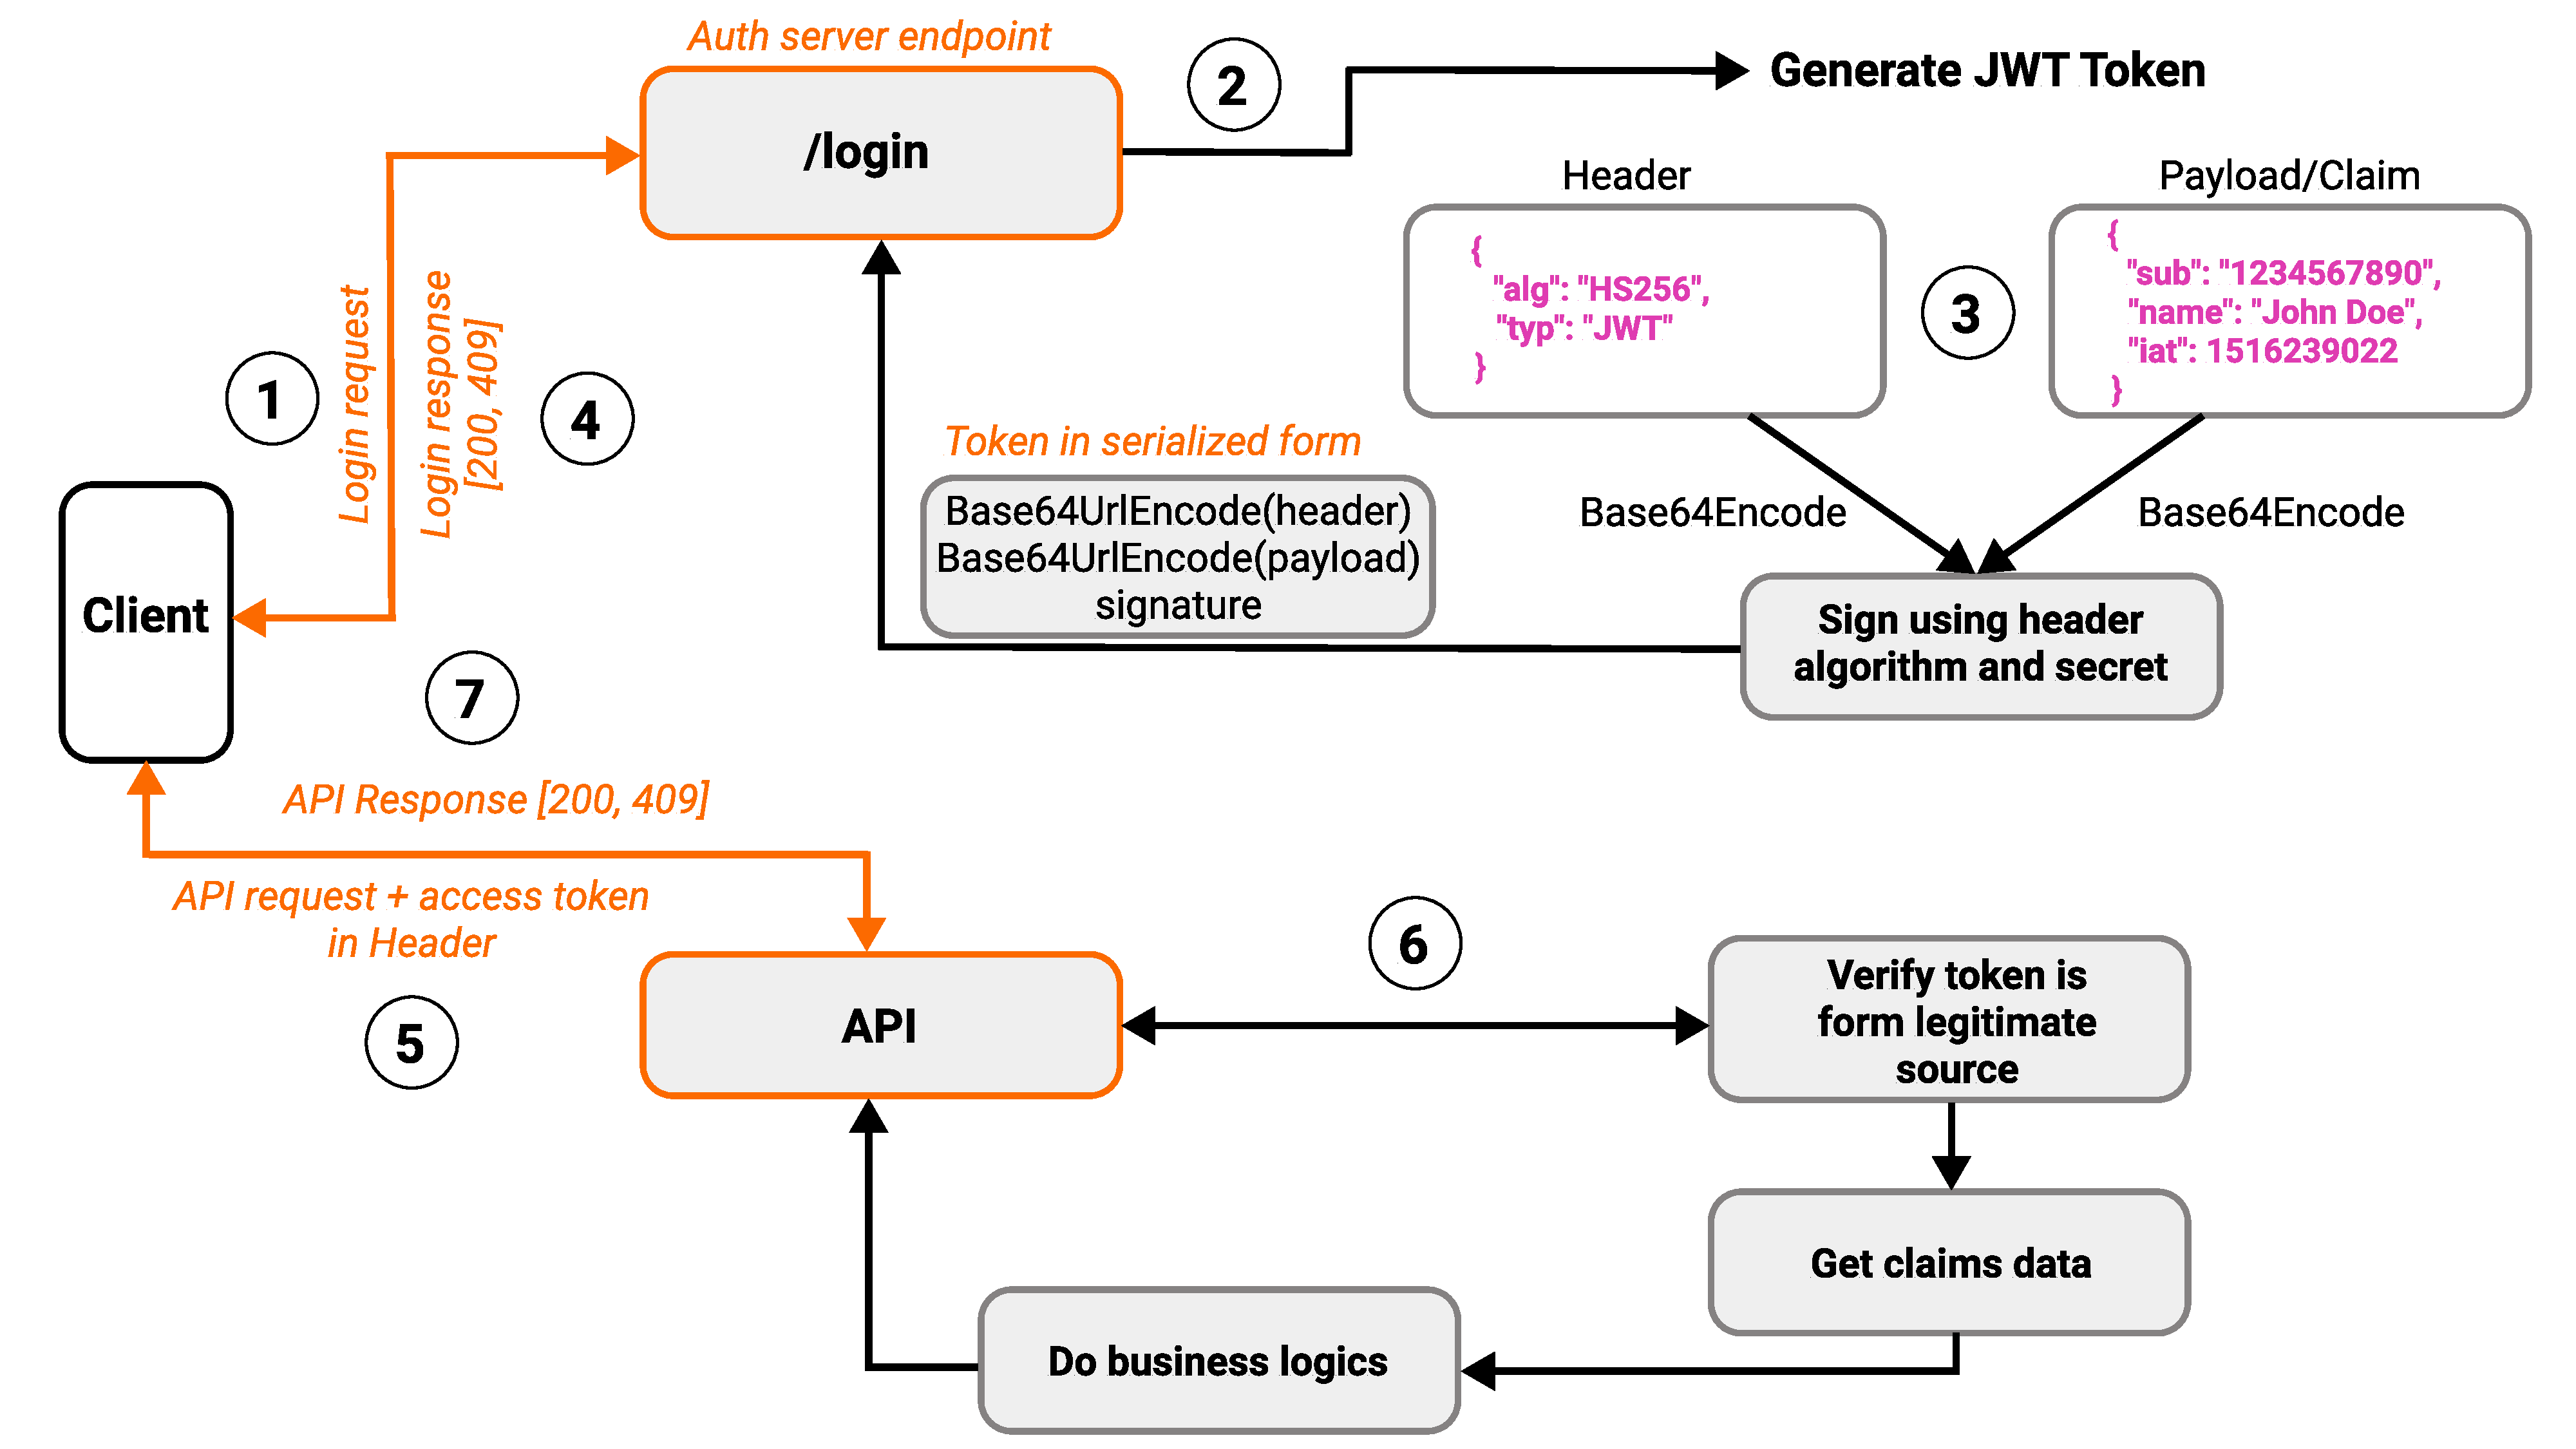
\includegraphics[width=1\textwidth]{Pictures/06_JWT_authorization_concept_diagram}
    \caption{JWT Authorization concept diagram.}\label{fig:figure3}
\end{figure}

By steps, the process is
\begin{itemize}
    \item \textbf{Step 1.} \textit{Client} application sends authentication request to
    the \textit{Auth server endpoint} provided user credentials in request body.
    \item \textbf{Step 2.} \textit{Auth server endpoint} responses to the \textit{Client} with the following
    HTTP response codes:
    \begin{itemize}
        \item \texttt{409CONFLICT}: Invalid credentials.
        \item \texttt{200SUCCESS}: Returns a pair of access and refresh tokens.
        \begin{itemize}
            \item \textbf{Step 3.} \textit{Auth server} generates a pair of access and refresh tokens
            \begin{itemize}
                \item \textit{Auth server} fetches user data and claims.
                \item \textit{Auth server} creates new session instance in database.
                \item \textit{Auth server} Base64 encodes access token's Header.
                \item \textit{Auth server} Base64 encodes access token's Payload.
                \item \textit{Auth server} generates access token's Signature using encoded token's
                Header and Payload signed by means of the \texttt{HMACSHA256} algorithm and secret.
            \end{itemize}
        \end{itemize}
    \end{itemize}
    \item \textbf{Step 4.} JWT access token in serialized form and refresh token in form of GUID are
    returned in response with \texttt{200SUCCESS} http status code to the \textit{Client} from the \textit{Auth server}.
    \item \textbf{Step 5.} \textit{Client} queries the \textit{API} providing access token as
    Bearer in request header.
    \item \textbf{Step 6.} \textit{API} validates the token claims in order to authorize user
    \begin{itemize}
        \item If authorized: \textit{API} handles the request, goes to \textbf{Step 7}.
        \item Otherwise: returns error with \texttt{401UNAUTHORIZED} http status code.
    \end{itemize}
    \item \textbf{Step 7.} \textit{} returns response with \texttt{200SUCCESS} or \texttt{409CONFLICT}
    http status codes to the client, according to business logic layer implementation.
\end{itemize}

\subsection*{7. End-to-end encryption}\label{subsec:end-to-end-encryption}
\textbf{Motivation.} End-to-end encryption is an encryption such that the only communicating parties
are able to decrypt the data.
It means that even system administrators are not able to decrypt the messages transmitted between parties
via their communication channel.
End-to-end encryption can be reached via numerous approaches.
Generally, there are two ways to implement E2E encryption
\begin{itemize}
    \item Sharing public key to be used in encryption of the secret message, then encryption is done by the
    public key's owner, so-called asymmetric encryption.
    For example, RSA algorithm.
    \item Asymmetric key exchange, where parties firstly exchanging the keys, then symmetrically encrypting
    the transferred data.
    For instance, Diffie--Hellman key exchange and AES256 encryption using common secret.
\end{itemize}
The most important aspect here is to securely store the secrets on the user's client application.
Due to storage issues, it doesn't make sense to implement E2E encryption for web
and desktop clients, like it is done in nowadays popular Telegram Messenger
[\cite{job2015modified,suvsanka2017security,lee2017security}].
Telegram uses the huge and heavy \texttt{MTProto 2.0} cryptographic protocol, based on DH key exchange and further AES256
symmetric encryption.
According to the project concerns, the E2E encryption via Diffie--Hellman key exchange and AES256
to be considered and implemented, the next section is about.

\textbf{Diffie–-Hellman key exchange.} Diffie--Hellman (DH) protocol is a method of asymmetric exchange
of the cryptographic keys for a group of two or more participants,
developed in 1976 by cryptographers Ralph Merkle, Whitfield Diffie and Martin Hellman.
In contrast to symmetric key exchange, the Diffie–-Hellman protocol eliminates the direct transfer of the shared secret
between the participants, each participant computes a shared secret with its own private-public key pair.
The Diffie–-Hellman protocol is based on a one-way function of the form

\begin{equation}
    A = G ^ a \bmod P \label{eq:equation}
\end{equation}

where $A$ is the user's public key,
$a$ is the user's private key,
$P=2Q+1$ is modulus, such that 2048 bits safe-prime because $Q$ is also prime,
$G$ is generator such that $G$ is primitive root modulo $P$.
We say that $G$ is primitive root modulo $P$ if for each $1 \leq a \leq P - 1$ the $A = G ^ a \bmod P$
is unique and belong to the set $\{1, 2, \dots, P-1\}$.
The period of such cyclic group $\mathbb{Z}_{P}$ is $P-1$ then.

Thus, the safety of the Diffie--Hellman protocol is based on the discrete logarithm problem, which is unsolvable
in polynomial time if the constants $G$ and $P$ are chosen correctly.
Graphically, the flow of the Diffie--Hellman protocol can be expressed through the
analogy with mixing paints, as below picture shows
\begin{figure}[H]
    \centering
    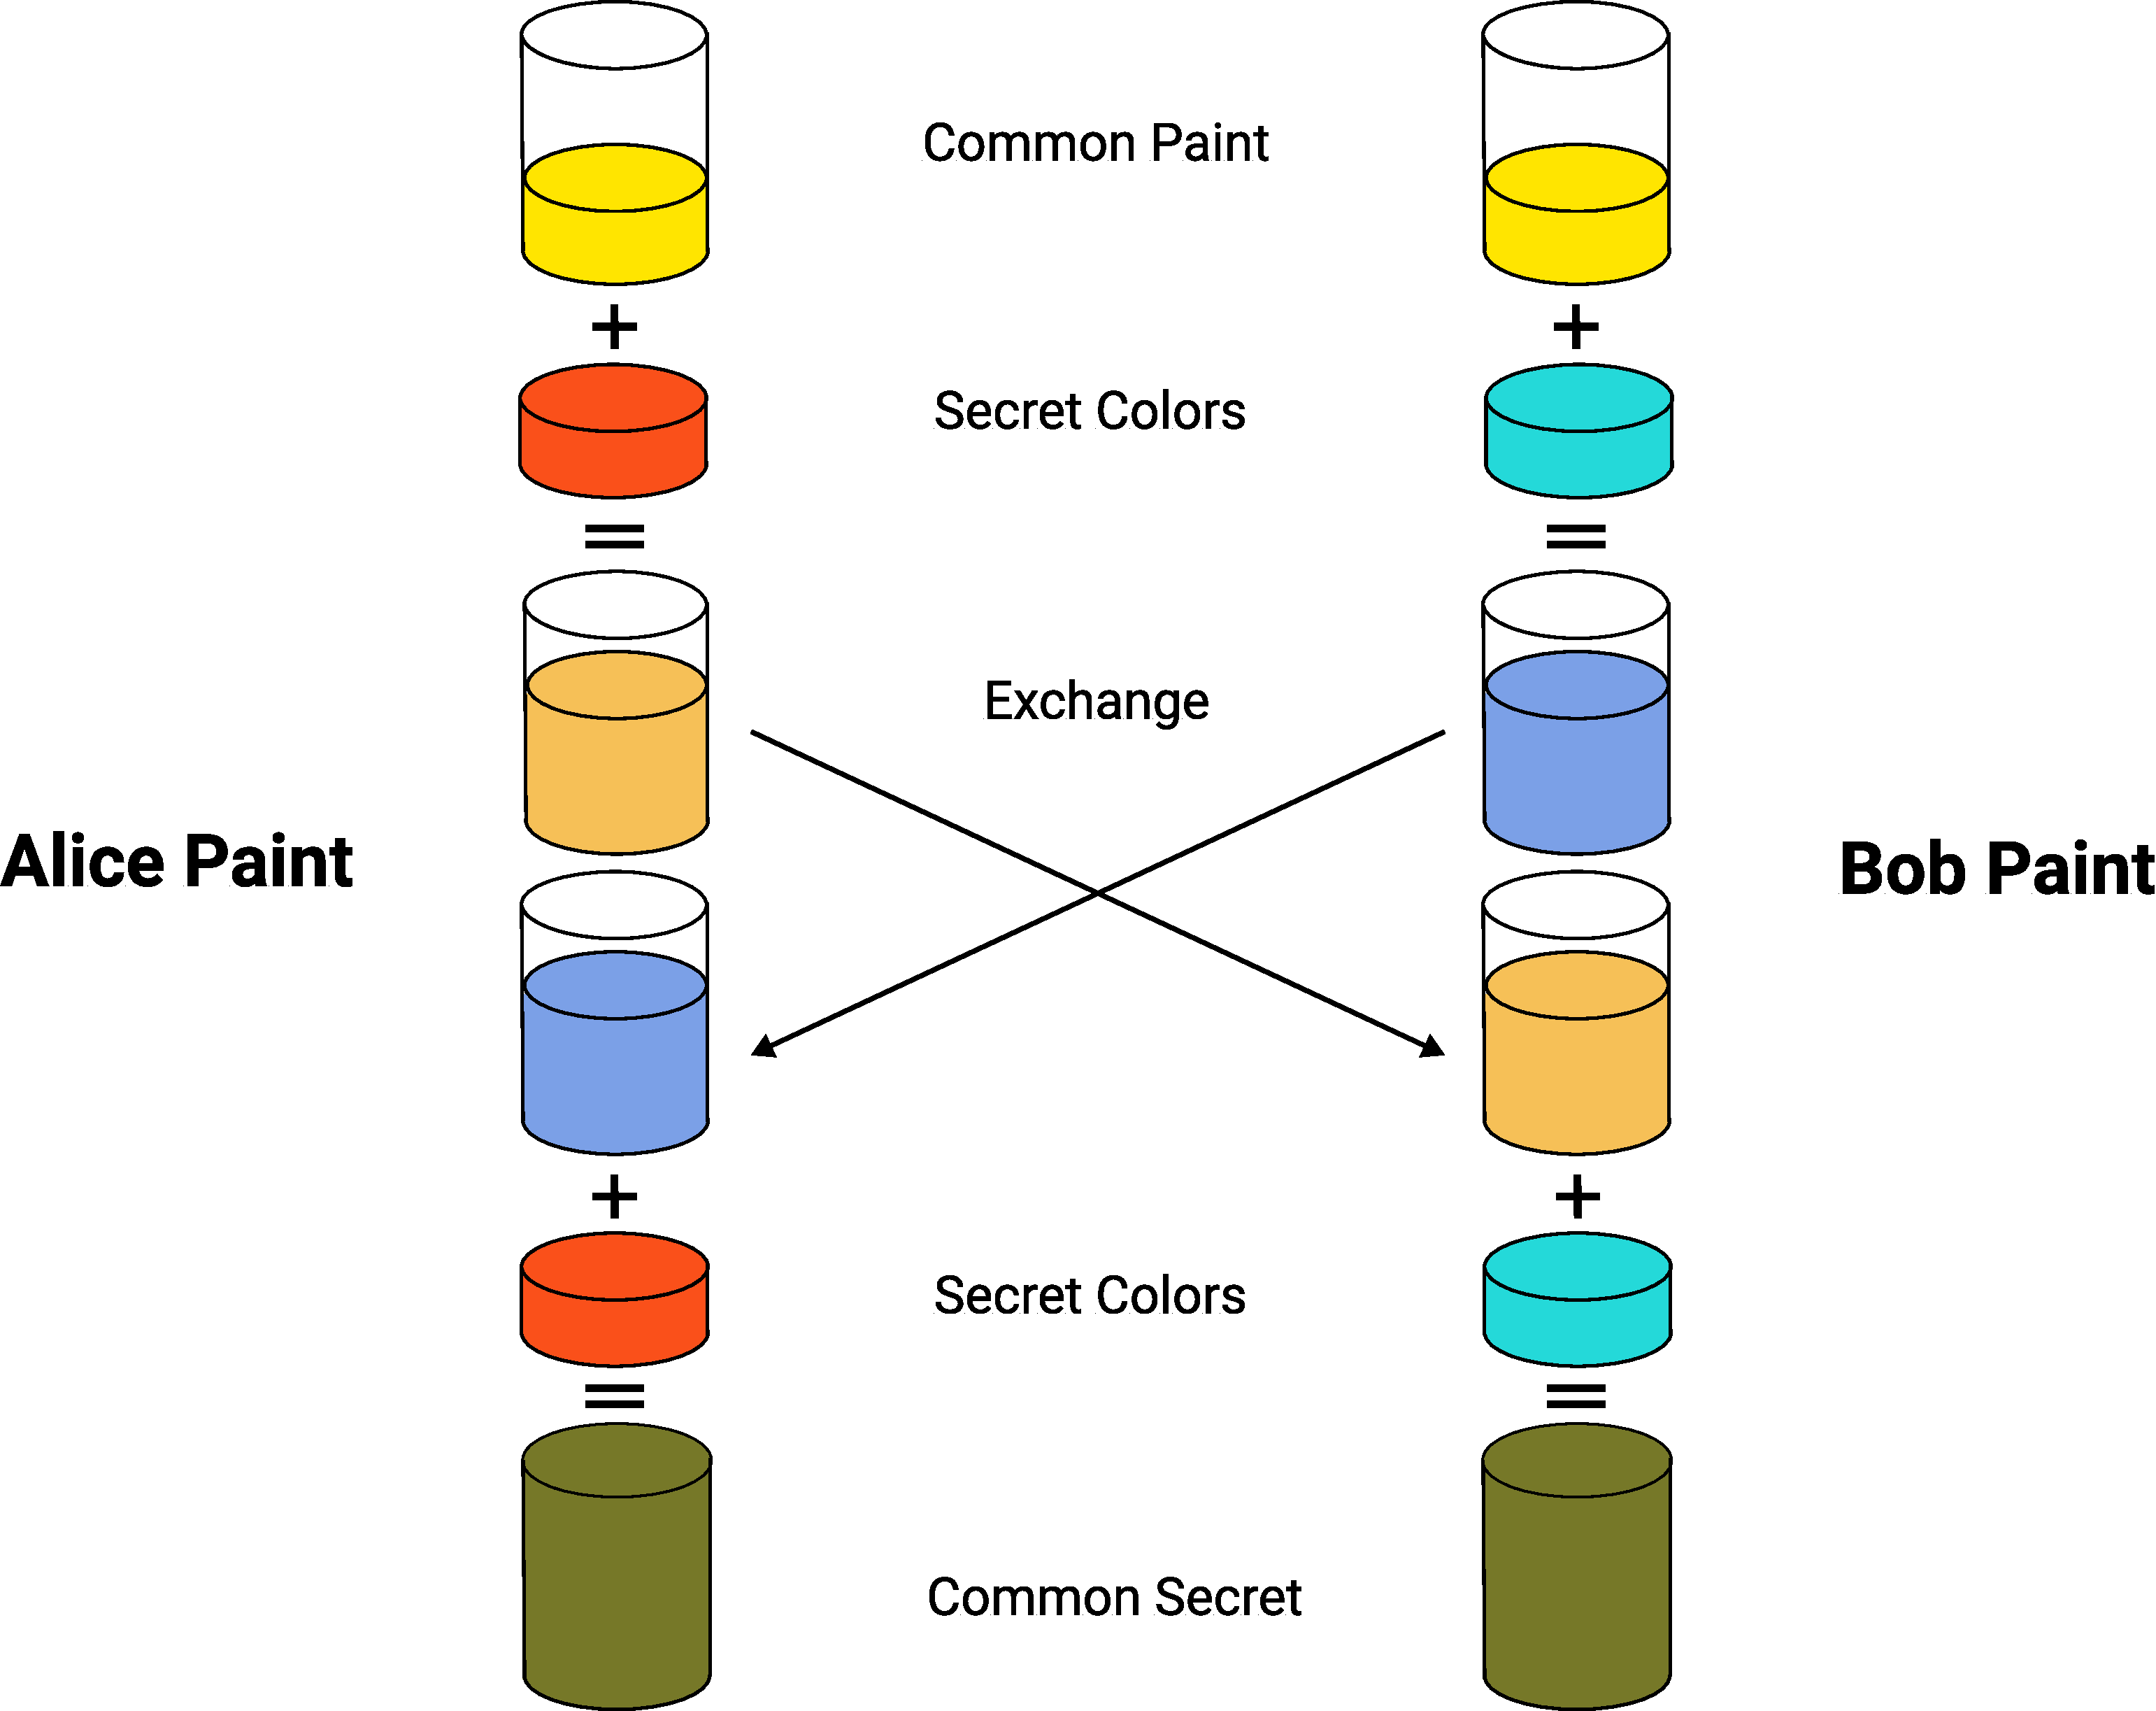
\includegraphics[width=1\textwidth]{Pictures/07_Diffie-Hellman_keyexchange_concept_diagram}
    \caption{Diffie–-Hellman key exchange concept diagram. Source: }\label{fig:figure4}
\end{figure}
In contrast to the Diffie–-Hellman based on discrete logarithm problem, there is an Elliptic Curve Diffie–-Hellman
key exchange, which based on the elliptic curve discrete logarithm problem.
Although, the idea is quite same, the difference only in that Elliptic Curve Diffie–-Hellman ensures the same safety
as discrete logarithm Diffie–-Hellman with lower value of the prime modulus $P$.
For instance, 521 bit modulus used in Elliptic Curve Diffie–-Hellman is equally safe as 2048 bit modulus in
discrete logarithm Diffie–-Hellman.
To summarize, the flow of Diffie–-Hellman key exchange is as follows
\begin{enumerate}
    \item Given 2048 bits prime modulus $P$ and generator $G$, such that $G$ is primitive root modulo $P$.
    \item Alice chooses her secret $a$.
    \item Alice sends to Bob her public key $A = G^a \bmod P$.
    \item Bob chooses his secret $b$.
    \item Bob sends to Alice his public key $B = G^b \bmod P$.
    \item Alice computes common secret $s = B^a \bmod P$.
    \item Bob computes common secret $s = A^b \bmod P$.
    \item Alice and Bob have arrived to the same value
    \begin{eqnarray}
        A^b \bmod P = G^{ab} \bmod P \\
        B^a \bmod P = G^{ba} \bmod P
    \end{eqnarray}
\end{enumerate}

\textbf{Implementation.} Although, the idea of DH key exchange looks quite simple, some remarks on the concrete
implementation should be added.
Firstly, it is necessary to implement the mechanism of key exchange request between two or more parties.
As it discussed above, each user has his own private-public keys pair, so in order to perform request between parties,
it should be implemented dedicate REST API endpoint, for instance the POST one \texttt{api/key-exchange-requests} which
takes the body of the form

\input{Files/post-keyexchange-body}

So, request sender generates on the client side a key pair, keeps private on in the file system and shares the public
in request to receiver.
Therefore, the second party has received the key exchange request.
In order to display all the key exchange requests awaiting the confirmation of decline decisions, it is worth to implement
another REST endpoint such that GET \texttt{api/key-exchange-requests}, so that requested party will have the list of
requests to proceed.
This endpoint may return the data structure like follows

\input{Files/get-keyexchangerequests-response}

Finally, requested party should be able to confirm or decline the key exchange request, the DELETE endpoint
\texttt{api/key-exchange-requests} should be implemented then.
The server is able to fetch the request thanks to the body endpoint takes

\input{Files/delete-keyexchangerequest-body}

Therefore, an identifier of awaiting request is passed to the server among with boolean value
indicating the confirmation.
Under the roof of this operation are also generation of private-public keys pair for the requested party and
generation of common secret stored in client's file system.
As result, the initial request sender receives a public key as confirmation from requested party.
Requested side may get all his public keys via the REST API using GET \texttt{api/public-keys}

\input{Files/get-publickeys-response}

Now requested participant is able to derive the common secret.
In order to provide an example, a simple command line interface is implemented.
We have used an Elliptic Curve Diffie–-Hellman implementation \texttt{ECDiffieHellmanCng Class} from the namespace
\texttt{System.Security.Cryptography} of the .NET base class library.
The \texttt{P-256} curve is used.

More precisely, the following CLI commands are implemented
\begin{itemize}
    \item \texttt{MangoAPI.DiffieHellmanConsole login SENDER\_EMAIL SENDER\_PASSWORD}
    \item \texttt{MangoAPI.DiffieHellmanConsole key-exchange RECEIVER\_ID}
    \item \texttt{MangoAPI.DiffieHellmanConsole key-exchange-requests}
    \item \texttt{MangoAPI.DiffieHellmanConsole confirm-key-exchange REQUEST\_ID}
    \item \texttt{MangoAPI.DiffieHellmanConsole print-public-keys}
    \item \texttt{MangoAPI.DiffieHellmanConsole create-common-secret RECEIVER\_ID}
\end{itemize}
Commands are self-explanatory, therefore we skip the detailed documentation on them.
An example of console output straightforward
\begin{figure}[H]
    \centering
    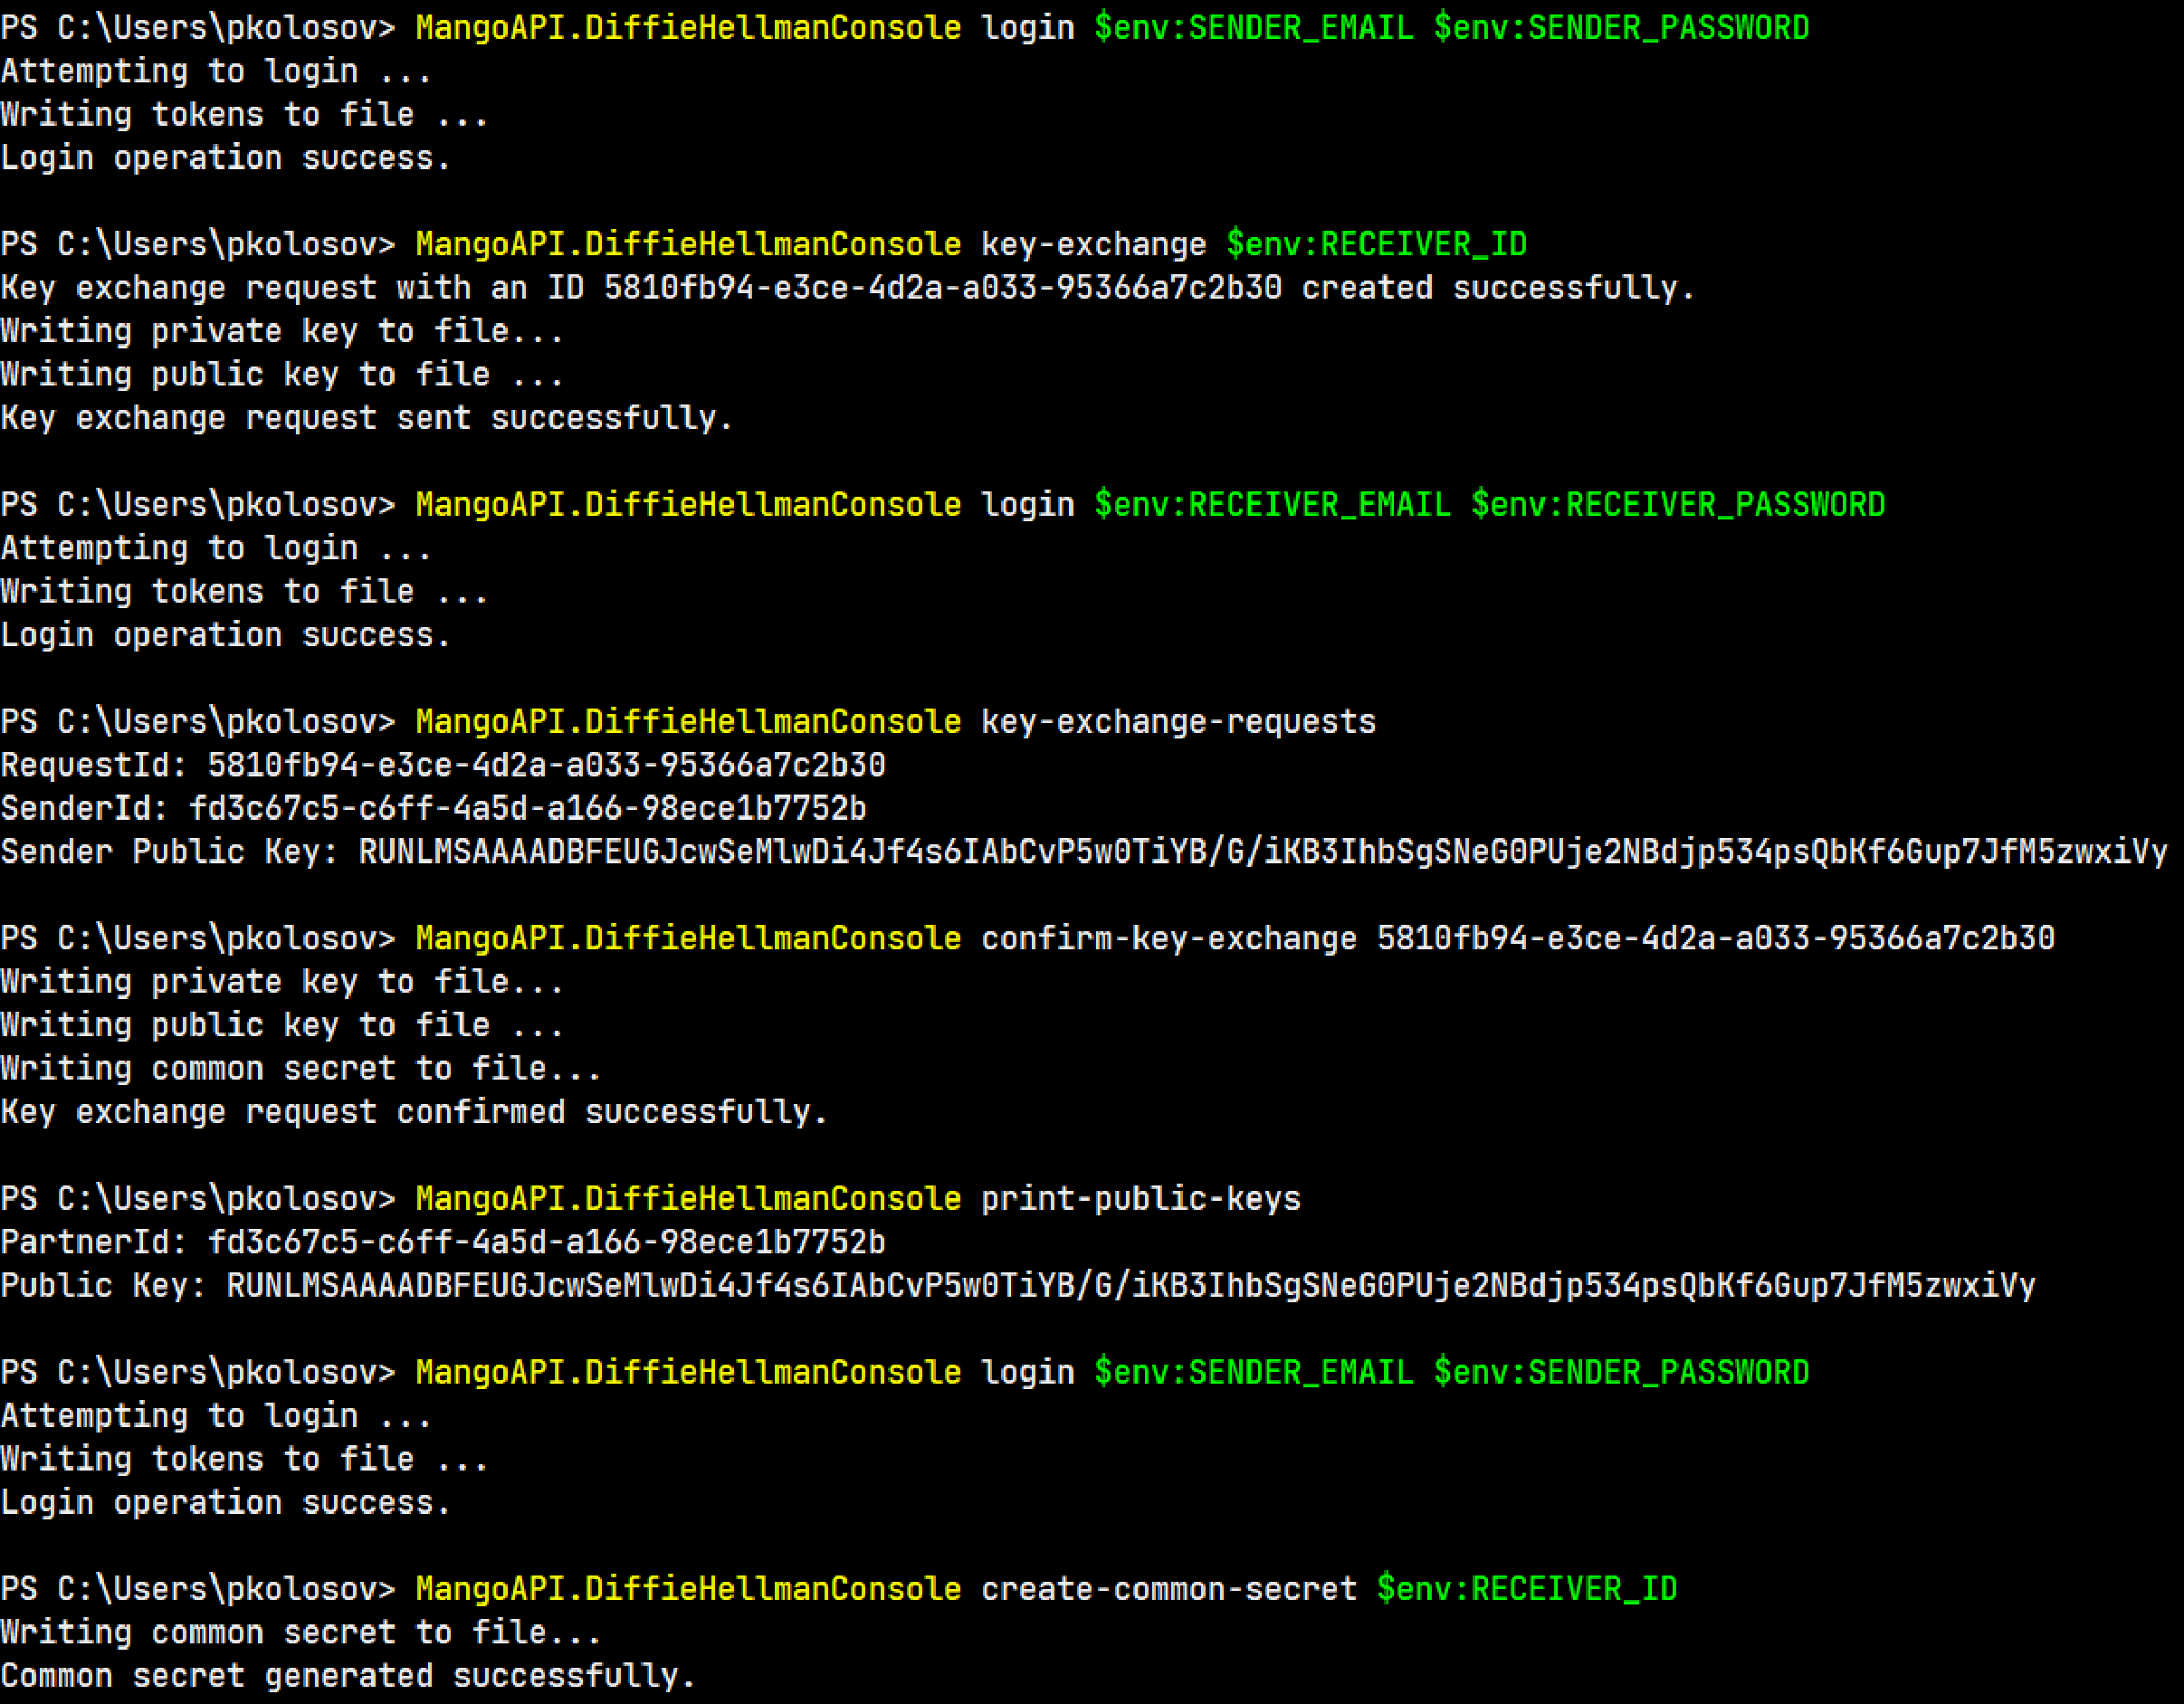
\includegraphics[width=1\textwidth]{Pictures/08_Diffie-Hellman_console_output}
    \caption{Diffie–-Hellman key exchange console output. Source: }\label{fig:figure7}
\end{figure}
Finally, both test accounts reached the same common secret.


\section{Project outcomes}\label{sec:project-outcomes}
In this section project outcomes are described.
Outcomes description includes the specifications of concrete functional requirements implemented along with the
graphic user interface screenshots.
Function requirements could be found in annexes.
We begin from the messenger's start page and continue further with user contacts component and user settings component.
\begin{figure}[H]
    \centering
    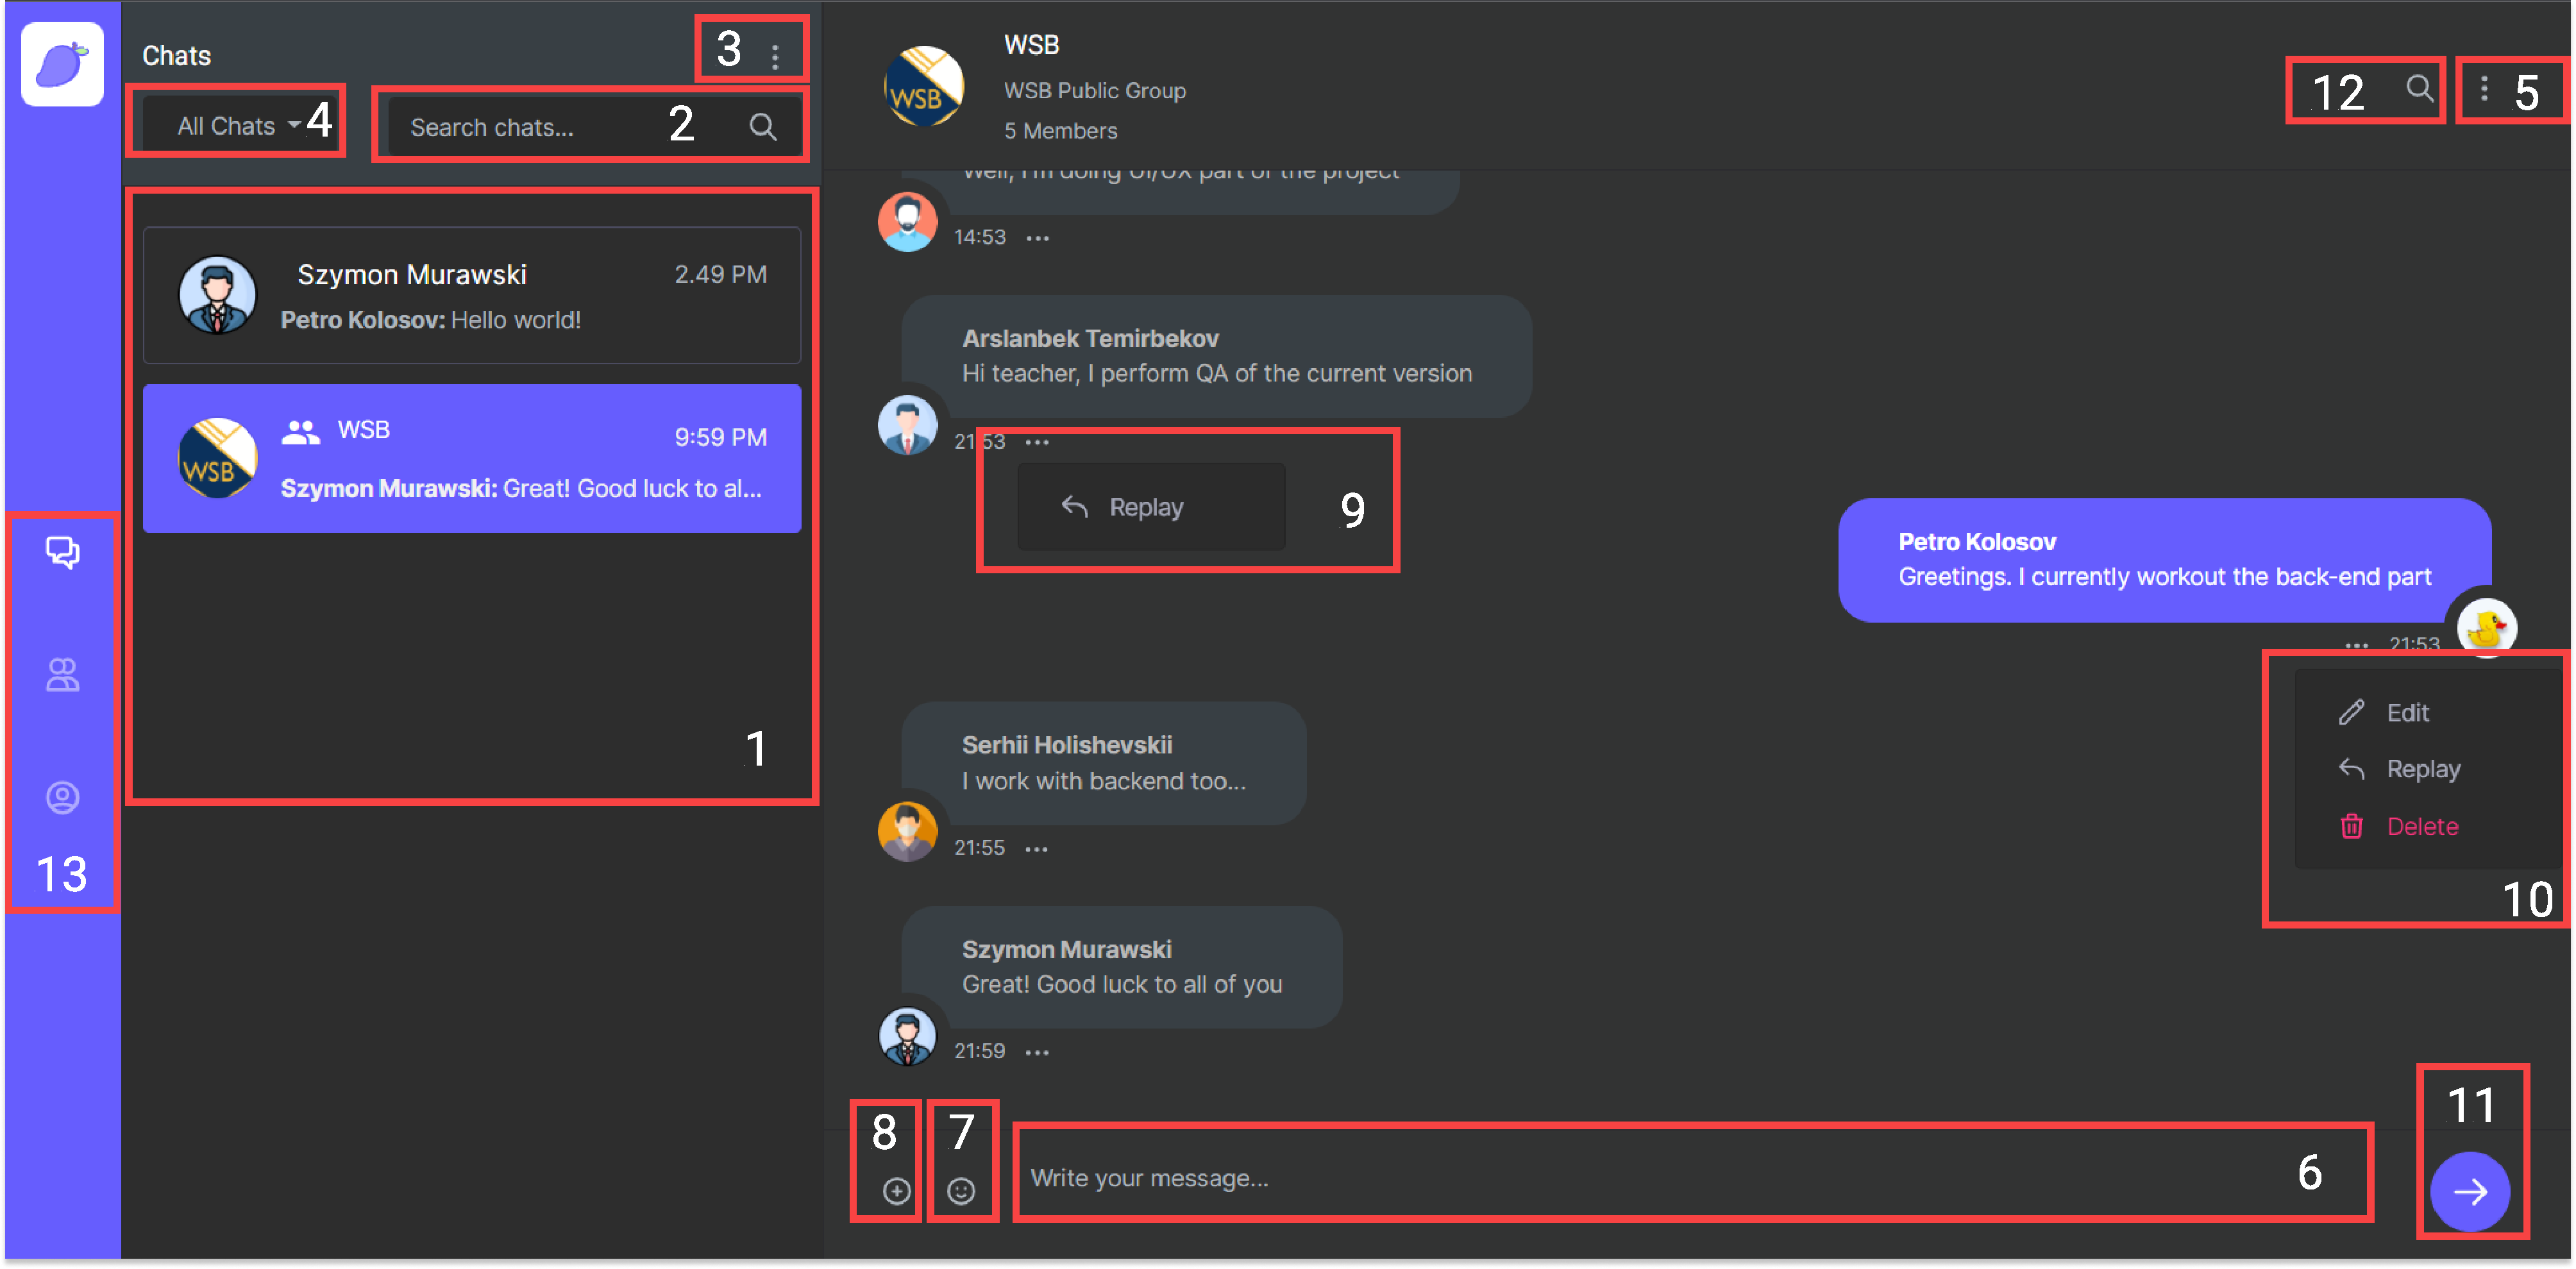
\includegraphics[width=1\textwidth]{Pictures/09_Messenger_startpage}
    ~\caption{Start page component screenshot. Source: [\cite{mango2021figma}].}\label{fig:figure5}
\end{figure}

\begin{enumerate}
    \item Element responsible for getting user's chats list so that functional requirement \textit{"As an authorized user,
        I want to view a message history of particular chat or group so that I see a list of my active chats on the UI"}
    is satisfied.
    \item Element responsible for searching chats by display name and displaying it so that functional requirements
    \begin{itemize}
        \item \textit{"As an authorized user, I want to search public groups by title so that I enter display name to specified field,
            click button "Search chats" and see results"}
        \item \textit{"As a registered user, I want to join public groups so that I click button "Join group"to join the group"}
    \end{itemize}
    are satisfied.
    \item Element responsible for creating groups so that functional requirement
    \textit{"As a registered user, I want to tap "Create channel" so that I create a new channel of the one of the types:
    Private channel, Public channel, Readonly channel"} is satisfied.
    \item Element responsible for filtering chats so that functional requirement \textit{"As an authorized user,
        I want to filter a message history of particular chat or group so that I see a filtered list of my active
        chats on the UI"} is satisfied.
    \item Element responsible for archiving and leaving from the particular chat, so that functional requirements
    \begin{itemize}
        \item \textit{"As registered user, I want to tap "Leave" so that I leave from specified chat or channel"}
        \item \textit{"As a registered user, I want to tap "Archive" so that I archive the specified chat or channel"}
        \item \textit{"As a registered user, I want to tap "Un-archive" so that I un-archive the specified archived chat or channel"}
    \end{itemize}
    are satisfied.
    \item Element responsible for entering the text and sending a message by enter, so that functional requirement
    \textit{"As an authorized user, I want to send a text message so that other members of the group see the message I sent"}
    is satisfied.
    \item Element responsible for adding emoji to message, so that functional requirement
    \textit{"As an authorized user, I want to add an emoji to the message so that other members of the group
    see the message with emoji I sent"} is satisfied.
    \item Element responsible for adding attachments to the message, so that functional requirement
    \textit{"As an authorized user, I want to add an attachment to the message so that other members of the group see the
    message with attachment I sent"} is satisfied.
    \item Element responsible for replying to message, so that functional requirement
    \textit{"As registered user, I want tap "Reply" so that I want reply to the particular message"} is satisfied.
    \item Element responsible for editing and deleting a message so that functional requirements
    \begin{itemize}
        \item \textit{"As an authorized user, I want to tap "Edit" on my message so that other members of the group
        see the message I edited"}
        \item \textit{"As an authorized user, I want to tap "Delete" on my message so that my message is deleted for
        all members of the group"}
    \end{itemize}
    are satisfied.
    \item Element responsible for sending message if message text field is not empty so that functional requirement
    \textit{"As an authorized user, I want to send a text message so that another user sees my message"}
    is satisfied.
    \item Element responsible for searching messages in the particular chat so that functional requirement
    \textit{"As an authorized user, I want to search messages in particular chat so that I see the results in
    messages window of the chat"} is satisfied.
    \item Element responsible for navigation about main page, contacts page and personal information page so that
    functional requirement
    \textit{"As an authorized user, I want to navigate between the pages so that there is a menu on the UI"} is satisfied.
\end{enumerate}

\begin{figure}[H]
    \centering
    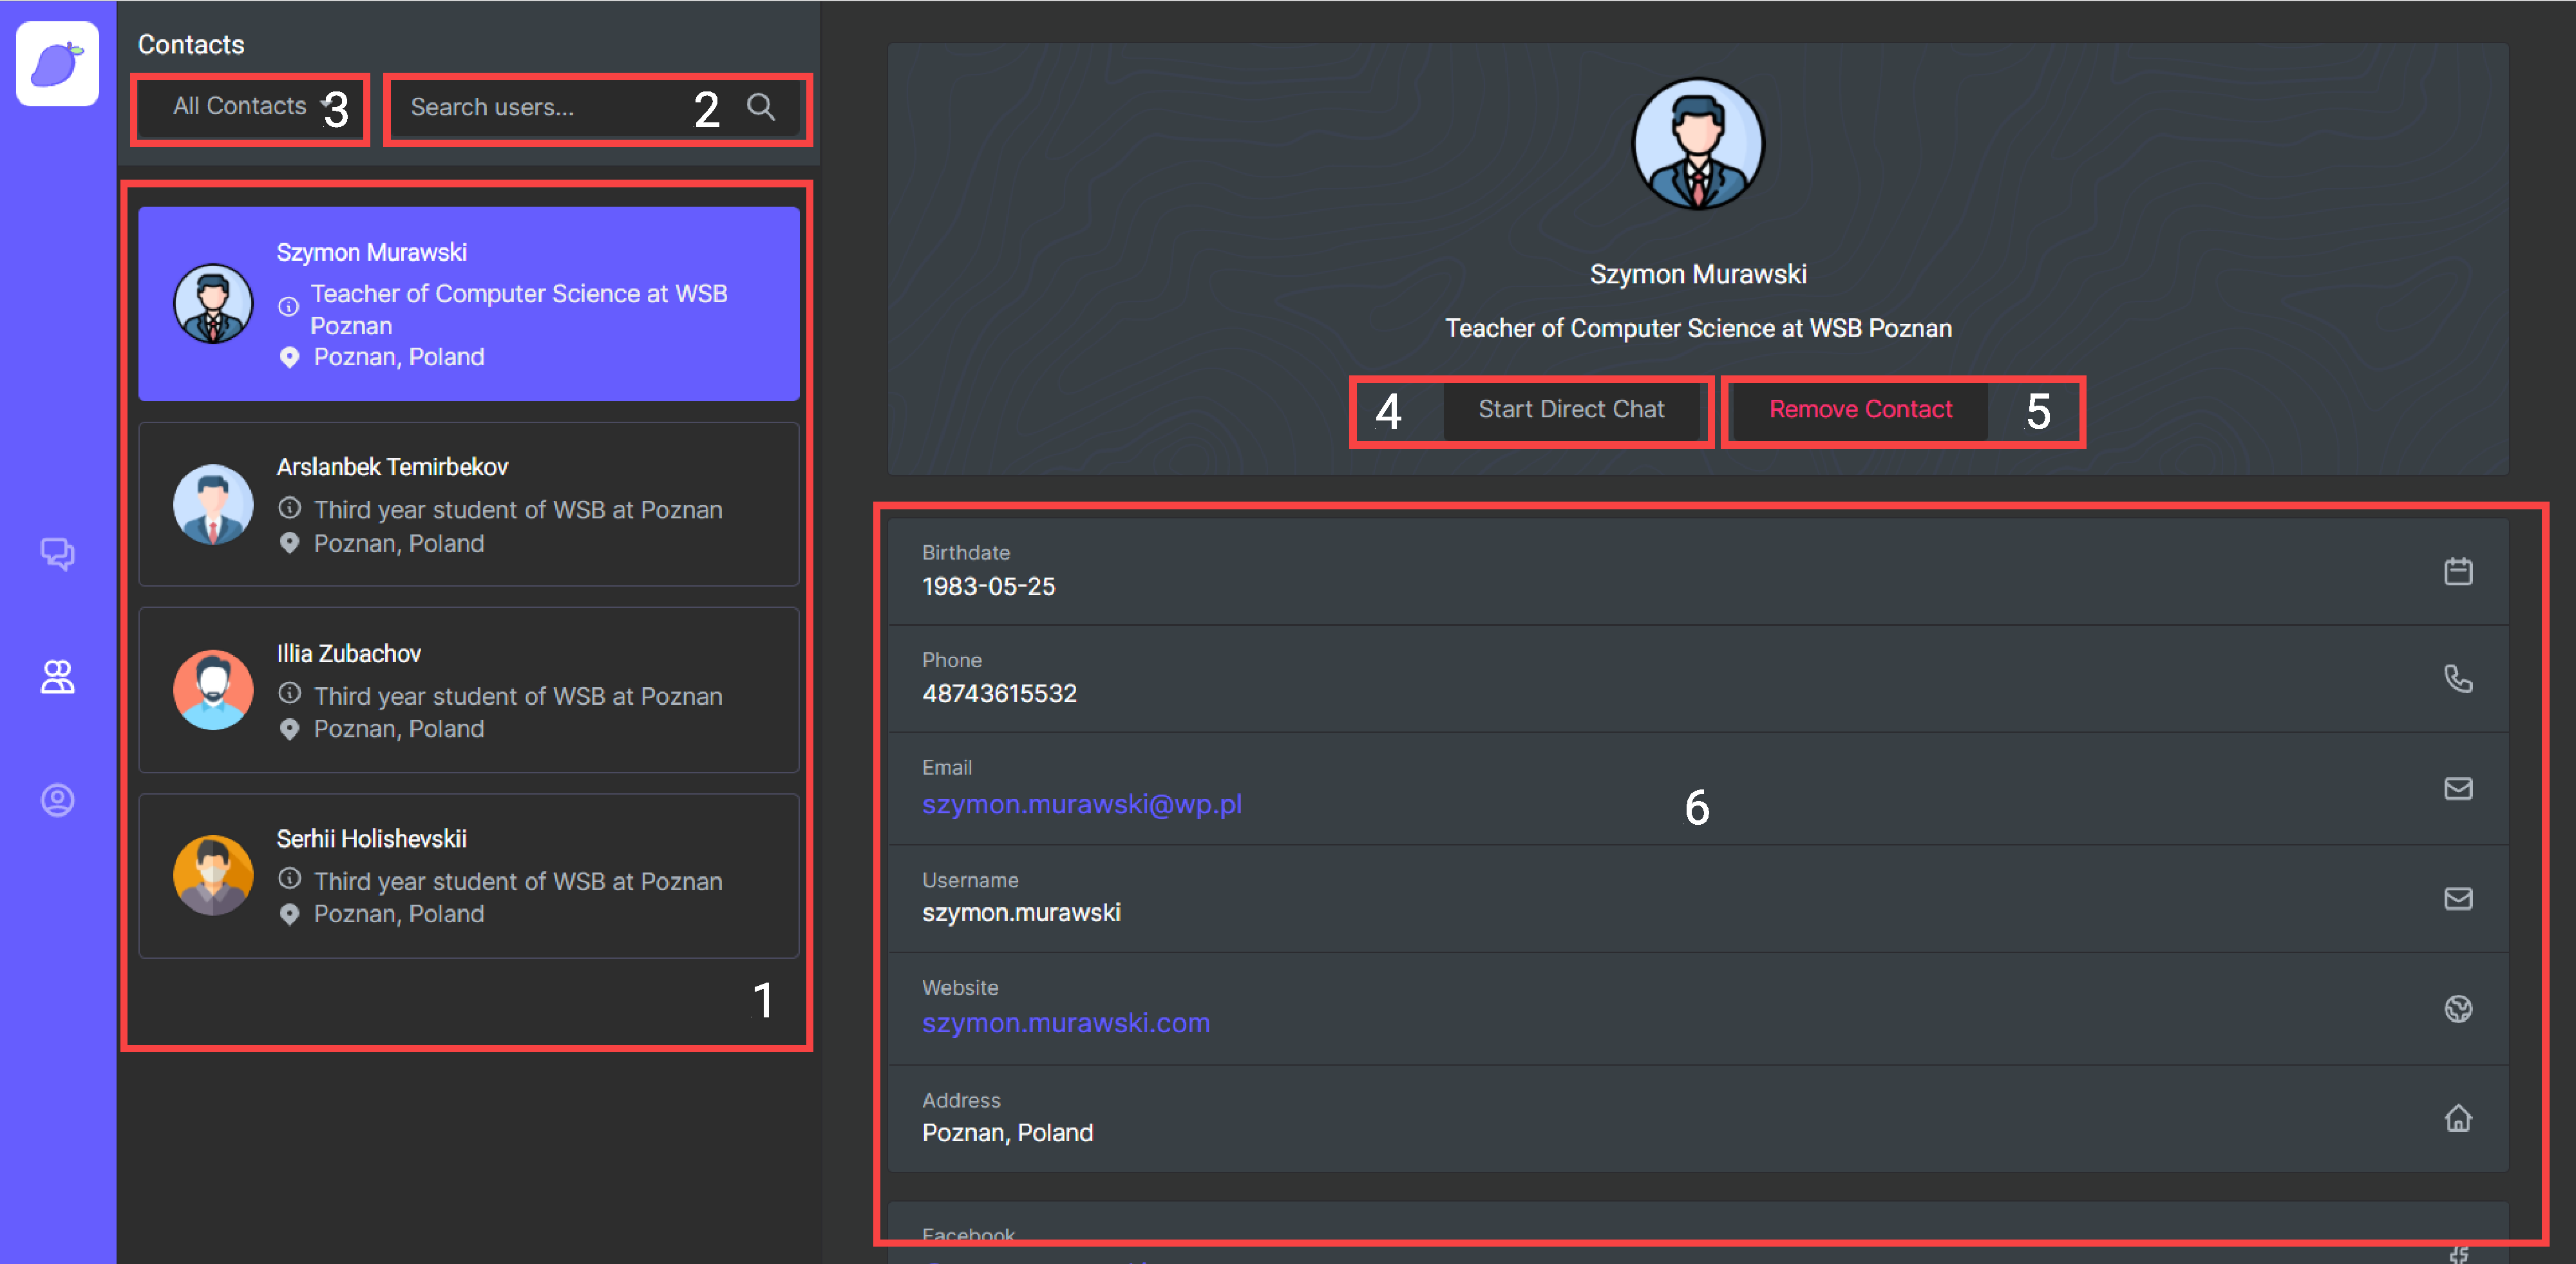
\includegraphics[width=1\textwidth]{Pictures/10_Messenger_manage_contacts}
    ~\caption{Manage contacts component screenshot. Source: [\cite{mango2021figma}].}\label{fig:figure10}
\end{figure}
\begin{enumerate}
    \item Element responsible for output user's contacts so that functional requirement
    \textit{"As an authorized user, I want to see my contact list so that there is a list of users
    who are my contacts"} is satisfied.
    \item Element responsible for searching users so that functional requirement
    \textit{"As an authorized user, I want to search users so that I write user display name or phone number
    of e-mail address to specified input, click "Search user" button and see
    results"} is satisfied.
    \item Element responsible for filtering contacts so that functional requirement
    \textit{"As an authorized user, I want to search users so that I write user display name or phone number of e-mail
    address to specified input, click "Search user" button and see results"} is satisfied.
    \item There is a button, clicking on which you can start chat with a specific user, so that functional requirement
    \textit{"As a registered user, I want to tap "Start direct chat" so that I create a new direct
    chat with specified user"} is satisfied.
    \item Element responsible for deleting user form contacts so that functional requirement
    \textit{"As an authorized user, I want to remove the user from my contact list so that I click "Remove contact"
    button on user profile and remove him from my contact list"} is satisfied.
    \item Element responsible for the output specified user's info so that functional requirement
    \textit{"As an authorized user, I want to tap on specified contact so that I want see user's information"}
    is satisfied.
\end{enumerate}

\begin{figure}[H]
    \centering
    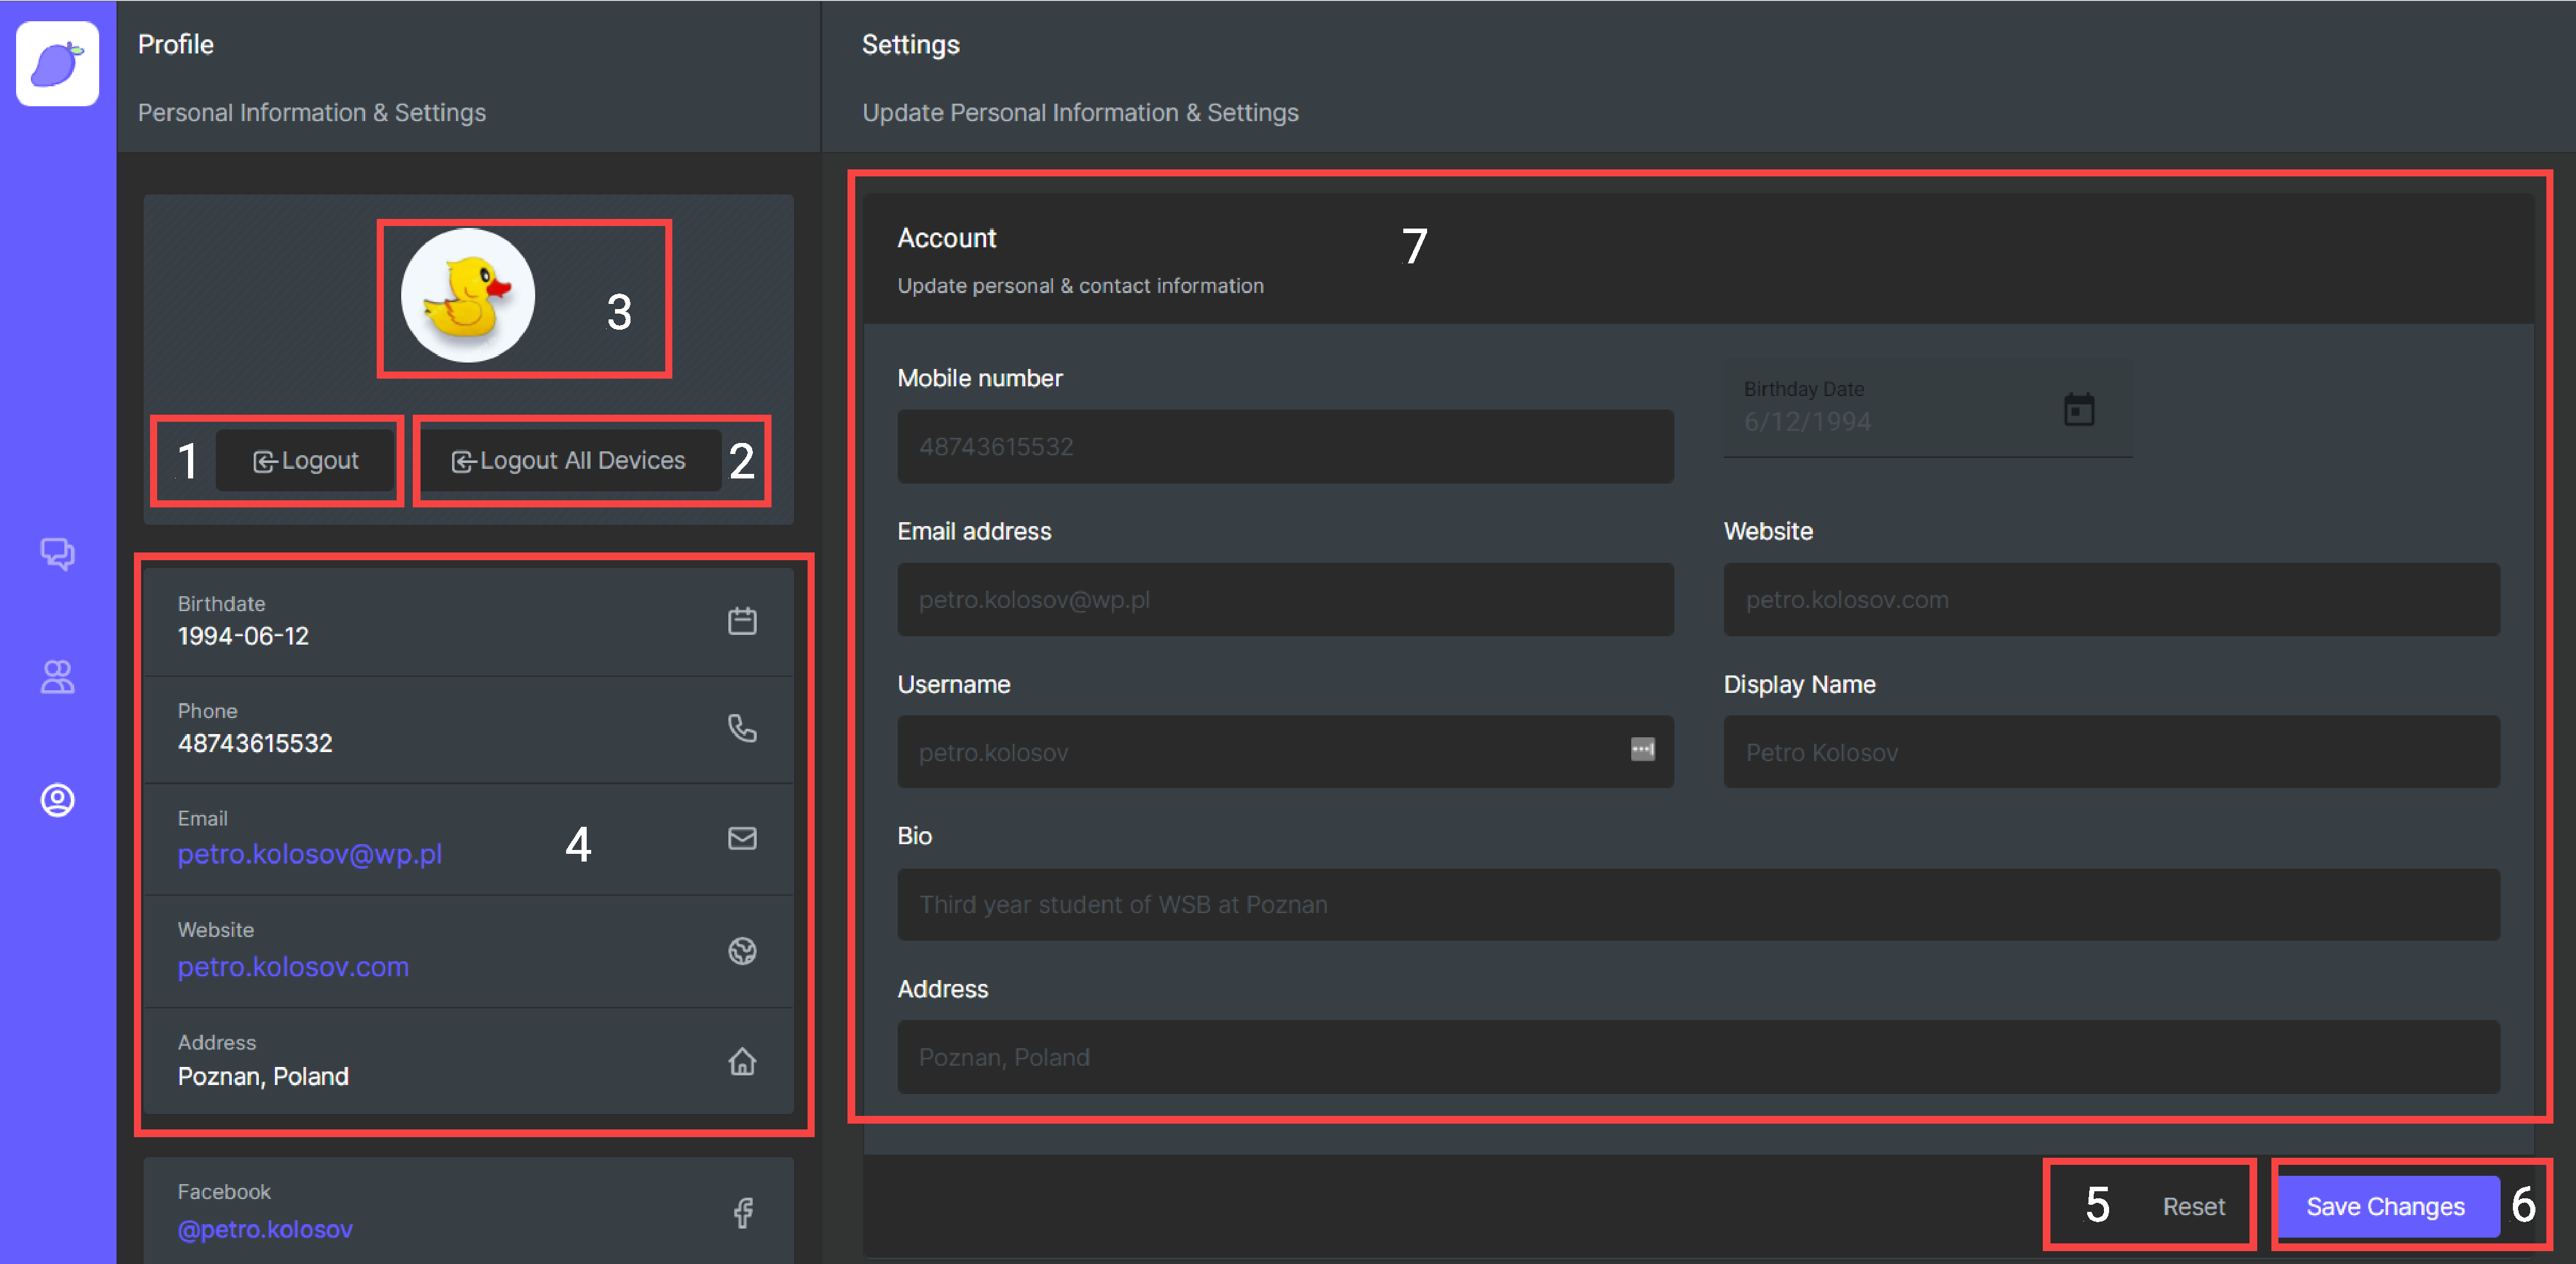
\includegraphics[width=1\textwidth]{Pictures/11_Messenger_account_settings}
    ~\caption{Account settings component screenshot. Source: [\cite{mango2021figma}]}\label{fig:figure11}
\end{figure}
\begin{enumerate}
    \item Element responsible for log out from specified device so that functional requirement
    \textit{"As an authorized user, I want to tap "Logout" button so that current device
    will be logged out from the system"} is satisfied.
    \item Element responsible for log out from all devices so that functional requirement
    \textit{"As an authorized user, I want to tap "Logout all" button so that all my authorized devices will be
    logged out from the system"} is satisfied.
    \item Element responsible for output user's avatar so that functional requirement
    \textit{"As an authorized user, I want to navigate to personal information page so that
    I want see my profile picture"} is satisfied.
    \item Element responsible for output user's information so that functional requirement
    \textit{"As an authorized user, I want to navigate to personal information page so that I want see my
    personal information"} is satisfied.
    \item Element responsible for reset updated personal information so that functional requirement
    \textit{"As an authorized user, I want to tap "Reset" so that I want reset my updated (not saved)
        personal information"} is satisfied.
    \item Element responsible for saving personal information so that functional requirement
    \textit{"As an authorized user, I want save my updated personal information so that users see it"}
    is satisfied.
    \item Element responsible for changing personal information so that functional requirement
    \textit{"As an authorized user, I want to update my personal information in profile settings so that other users
    my updated personal information"} is satisfied.
\end{enumerate}
Finally, we attach the list of technologies was used during an implementation of the project.
List of technologies are separated by categories is as follows
\begin{itemize}
    \item \textbf{SDK}: .NET Core 5.0
    \item \textbf{Backend:} ASP.NET Web API
    \item \textbf{Database}
    \begin{itemize}
        \item SQL Database: PostgreSQL 13
        \item ORM: Entity Framework Core 5.0
    \end{itemize}
    \item \textbf{Authorization}
    \begin{itemize}
        \item JWT Library: System JWT 6.8
        \item JWT Library: System Tokens 6.11
        \item JWT Bearer: Microsoft Jwt Bearer 5.0
    \end{itemize}
    \item \textbf{Business Logic}
    \begin{itemize}
        \item MediatR 9.0
        \item Fluent Validation 10.2
        \item AutoMapper 10.1
    \end{itemize}
    \item \textbf{Presentation}
    \begin{itemize}
        \item Documentation: Swashbuckle 6.1
        \item Realtime Communication: SignalR 2.4
        \item Frontend Development: Angular 11.2.7
        \item Desktop Development: ElectronJS framework.
        \item Mobile Development: WebView
    \end{itemize}
    \item \textbf{Unit and Integration Testing}
    \begin{itemize}
        \item Testing Framework: NUnit 3.13
        \item Testing Auxiliary: Moq 4.16
        \item Testing Auxiliary: FluentAssertions 6.0.0
    \end{itemize}
    \item \textbf{Static Code Analysis}: SonarQube 8.9.2 LTS
    \item \textbf{Containerization}: Docker 3.6
    \item \textbf{Continuous Integration}: GitHub Actions, Heroku, Azure
    \item \textbf{Programming languages}: C\#, SQL, TypeScript, Kotlin
    \item \textbf{Tools}: Microsoft Visual Studio, JetBrains Rider, Visual Studio Code, WebStorm.
\end{itemize}


\section{Usefulness of project}\label{sec:usefulness-of-project}
The project may be used as corporate messenger in closed scope of some company under VPN as cheaper alternative to the
nowadays popular Microsoft Teams.
The system provides independence from the centralized Microsoft's products.



\section{Project self-evaluation}\label{sec:project-self-evaluation}
In this section each of the project's Authors describes his or her skills and competencies that
were developed while working on the project and identifies issues encountered while working on the project.

\begin{itemize}
    \item \textbf{Petro Kolosov.} Petro has obtained an experience in best practice
    in context of modern web applications.
    Got familiar with cryptographic protocols and approaches as well as encryption algorithms,
    both symmetric and asymmetric.
    Also, increased his knowledge in software modules architecture.
    Has worked with technologies: ASP.NET Web API, PostgreSQL 13, Entity Framework Core, ElectronJS,
    NUnit, Moq, SonarQube, Docker, Heroku, Azure, C\#, SQL, TypeScript.
    Moreover, familiarized himself with CI/CD practices, precisely, writing pipelines for various environments,
    like Azure.
    Faced the following issues
    \begin{itemize}
        \item Has been engaged in backend implementation using ASP .NET
        \item Written CI/CD pipelines for Angular Front-End Application, Backend,
        Thesis document deployment on GitHub Pages
        \item Discussed database structure
        \item Written thesis document using \LaTeX
        \item Set up environments: QA, Dev.
        Where QA is deployed on Heroku and Dev environment is deployed on Azure.
    \end{itemize}
    \item \textbf{Serhii Holishevskii.} Serhii has obtained an experience in best practice
    in context of modern web applications.
    Got familiar with cryptographic protocols and approaches as well as encryption algorithms,
    both symmetric and asymmetric.
    Also, increased his knowledge in software modules architecture.
    Has worked with technologies: ASP.NET Web API, PostgreSQL 13, Entity Framework Core, ElectronJS,
    NUnit, Moq, SonarQube, Docker, Heroku, Azure, C\#, SQL, TypeScript.
    Faced the following issues
    \begin{itemize}
        \item Has been engaged in backend implementation using ASP .NET
        \item Written CI/CD pipelines for Angular Front-End Application, Backend,
        Thesis document deployment on GitHub Pages
        \item Discussed database structure
        \item Written thesis document using \LaTeX
        \item Implemented mobile client application using WebView
        \item Front-end development using Angular and TypeScript
    \end{itemize}
    \item \textbf{Illia Zubachov.} Illia has gained a knowledge of modern frontend web frameworks such as
    Angular, Angular materials.
    Got experience working with Typescript programming language.
    Also, has familiarized himself with QA best practices and approaches.
    Worked with technologies: TypeScript, Angular, ElectronJS, Docker.
    Faced the following issues
    \begin{itemize}
        \item Front-end development using Angular and TypeScript
        \item Unit tests writing for backend
        \item QA of the front end project
        \item Discussed database structure
        \item Written thesis document using \LaTeX
    \end{itemize}
    \item \textbf{Arslanbek Temirbekov.} Arslanbek has gained a knowledge of modern frontend web frameworks such as
    Angular, Angular materials.
    Got experience working with Typescript programming language.
    Also, has familiarized himself with QA best practices and approaches.
    Worked with technologies: TypeScript, Angular, ElectronJS, Docker.
    \begin{itemize}
        \item Front-end development using Angular and TypeScript
        \item Integration tests writing for backend
        \item QA of the front end project
        \item Discussed database structure
        \item Written thesis document using \LaTeX
    \end{itemize}
\end{itemize}
%    \chapter{Impelentation}\label{ch:impelentation}


\section{Project tasks}\label{sec:project-tasks}
\begin{description}
    \item \hspace*{8mm}\textbf{Task 1.}\\[5mm]
    \begin{tabular}{|p{5cm}|p{7cm}|}
        \hline
        Task name                                                                       & \\
        \hline
        Entities involved in the fulfilment of the task (max: 5 sentences)              & \\
        \hline
        Task completion outcomes (preparation / decisions / technical / dossier, etc. ) & \\
        \hline
        Star date of task execution                                                     & \\
        \hline
        End date of task execution                                                      & \\
        \hline
    \end{tabular}
    \item \hspace*{8mm}\textbf{Task 2.}\\[5mm]
    \begin{tabular}{|p{5cm}|p{7cm}|}
        \hline
        Task name                                                                       & \\
        \hline
        Entities involved in the fulfilment of the task (max: 5 sentences)              & \\
        \hline
        Task completion outcomes (preparation / decisions / technical / dossier, etc. ) & \\
        \hline
        Star date of task execution                                                     & \\
        \hline
        End date of task execution                                                      & \\
        \hline
    \end{tabular}
    \item \hspace*{8mm}\textbf{Task 3.}\\[5mm]
    \begin{tabular}{|p{5cm}|p{7cm}|}
        \hline
        Task name                                                                       & \\
        \hline
        Entities involved in the fulfilment of the task (max: 5 sentences)              & \\
        \hline
        Task completion outcomes (preparation / decisions / technical / dossier, etc. ) & \\
        \hline
        Star date of task execution                                                     & \\
        \hline
        End date of task execution                                                      & \\
        \hline
    \end{tabular}
    \item \hspace*{8mm}\textbf{Task 4.}\\[5mm]
    \begin{tabular}{|p{5cm}|p{7cm}|}
        \hline
        Task name                                                                       & \\
        \hline
        Entities involved in the fulfilment of the task (max: 5 sentences)              & \\
        \hline
        Task completion outcomes (preparation / decisions / technical / dossier, etc. ) & \\
        \hline
        Star date of task execution                                                     & \\
        \hline
        End date of task execution                                                      & \\
        \hline
    \end{tabular}
\end{description}

%\textbf{Task 1} \\
%
%\begin{tabular}{|p{5cm}|p{7cm}|}
%    \hline
%    Task name                                                                            & \\
%    \hline
%    Entities involved in the fulfilment of the task (max: 5 sentences)                   & \\
%    \hline
%    Task completion outcomes (preparation / decisions / technical / dossier, etc. )      & \\
%    \hline
%    Star date of task execution                                                          & \\
%    \hline
%    End date of task execution                                                           & \\
%    \hline
%\end{tabular} \\
%
%\textbf{Task 2} \\
%
%\begin{tabular}{|p{5cm}|p{7cm}|}
%    \hline
%    Task name                                                                            & \\
%    \hline
%    Entities involved in the fulfilment of the task (max: 5 sentences)                   & \\
%    \hline
%    Task completion outcomes (preparation / decisions / technical / dossier, etc. )      & \\
%    \hline
%    Star date of task execution                                                          & \\
%    \hline
%    End date of task execution                                                           & \\
%    \hline
%\end{tabular}


\section{Project implementation}\label{sec:project-implementation}
[Please develop the theoretical assumptions of the project, including notes; present the empirical part of the project – research results and conclusions, as well as subject-matter description, etc.
Please present computations and calculations, if any, in annexes.
Please do not change the names of the points below.
There is no predefined structure within individual points.
Also, additional parts, forming individual points, can be enumerated according to your own concept.
The theoretical and empirical part should not exceed 50,000 characters.
Please use Times New Roman font, 12 pts, 1.5 spacing.] \\

\begin{enumerate}
    \item Theoretical assumptions
    \item Description of facts
    \item Empirical research
\end{enumerate}


\section{Project outcomes}\label{sec:project-outcomes}
[Please describe the achieved outcomes of the project.
If possible, please provide figures showing the described outcomes.
Please confront them with the objectives of the project.
This part should be between 2000 and 10,000 characters long.
Please use Times New Roman font, 12 pts, 1.5 spacing.
Full description of solutions that were worked out and project outcomes, if any, should be presented in annexes.]


\section{Usefulness of project}\label{sec:usefulness-of-project}
[Please justify how this project is useful (how the project can be used in practice).
The description should not exceed 6000 characters.
Please use Times New Roman font, 12 pts, 1.5 spacing.]


\section{Project self-evaluation}\label{sec:project-self-evaluation}
[Each of the project’s Authors describes his or her skills and competencies that were developed while working on the project and identifies issues encountered while working on the project.
If during the work on the project the team had not completed any tasks planned earlier, or omitted them altogether, please specify what were these tasks and why they had not been completed.
This part should not exceed 6000 characters.
Please use Times New Roman font, 12 pts, 1.5 spacing.]


\section{Material and bibliography used to carry out the project}\label{sec:material-and-bibliography-used-to-carry-out-the-project}
[Please enumerate sources used by the team during the work on the project (as per the applying layout, Times New Roman font, 12 pts., 1.5 spacing).]


\section{List of annexes}\label{sec:list-of-annexes}
[In this place you should list all additional documents, e.g. preprinted forms, data sets, financial statements, survey templates, diagrams,
    concepts, strategies, studies, analyses, procedures, regulations, technical documents, plans, models, etc. which significantly contributed to the project.
Please prepare all annexes in accordance with the template in place.
Please use Times New Roman font, 12 pts, 1.5 spacing.
All annexes form an integral part of the project.]


%    \chapter*{System Requirements}\label{ch:system-requirements}
\addcontentsline{toc}{chapter}{System Requirements}

In previous sections we have briefly discussed Instant Messaging System, mainly from security and user privacy aspects.
Prior to software module implementation, it is essentially important to define the functionality module will obtain.
In this section we discuss functional and non-functional requirements of secure instant messaging system from customer's prospective.

Generally, there are three forms of software product requirements: business, functional, and non-functional.
Business requirements [\cite{dilworth2007creation}] typically answer how the product will address the needs of your company and its users.
They also reveal the business model of the app and what problems it can solve.
Functional requirements [\cite{malan2001functional}] are about functionalities that will be implemented in the application.
Non-functional requirements [\cite{chung2012non}] describe how these functionalities will be implemented.

\section{Functional Requirements}\label{sec:functional-requirements}
To compete with successful and commonly used instant messaging platforms, your service has to offer great functionality.
So first, let’s define the core features of a messaging app.
\begin{itemize}
    \item Registration
    \item Authentication
    \item Authorization
    \item Adding contacts
    \item Sending messages and media to individuals
    \item Creating groups
    \item Sending messages and media to groups user stories
    \item Viewing message history
    \item Profile settings
\end{itemize}
Note that Authentication [\cite{burrows1989logic}] means confirming your own identity,
whereas Authorization [\cite{fagin1978authorization}] means being allowed access to the particular part of the system.

\subsection{Registration user stories}\label{subsec:registration}
\begin{itemize}
    \item As an unregistered user, I want to tap “register” so that I can see the registration form.
    \item As an unregistered user, I want to use my phone number to register so that my account is tied to my phone number.
    \item As an unregistered user, I want to use my e-mail to register so that my account is tied to my phone number.
    \item As an unregistered user, I want to add a display name during registration so that other users can find
    my account not only by my phone number or e-mail.
    \item As an unregistered user, I want to choose how to receive the registration confirmation via SMS or e-mail
    so that notification is sent by SMS or e-email.
    \item As an unregistered user, I want to receive the registration confirmation via SMS or Email so that
    I can activate my account.
\end{itemize}

\subsection{Authentication user stories}\label{subsec:authentication-user-stories}
\begin{itemize}
    \item As an un-authenticated user, I want to authenticate myself using both combinations email-password
    and phone-password so that I use the specified form with two inputs.
    \item As an authenticated user, I want my session on each device to least 7 days
    so that after 7 days of inactivity device will be logged out automatically.
\end{itemize}

\subsection{Adding contacts user stories}\label{subsec:adding-contacts}
\begin{itemize}
    \item As an authorized user, I want to add other user to my contact list so that each user profile has a dedicated button.
    \item As an authorized user, I want to remove the user from my contact list so that each contact profile has a dedicated button.
    \item As an authorized user, I want to send message to the user from my contact list so that each contact profile has a dedicated button.
\end{itemize}

\subsection{Sending messages and media to individuals user stories}
\label{subsec:sending-messages-and-media-feature-user-stories}
\begin{itemize}
    \item As an authorized user, I want to send a text message so that another user sees my message.
    \item As an authorized user, I want to send a document so that another user sees the document I sent.
    \item As an authorized user, I want to tap "Edit" on my message, so that I edit the message sent by myself.
    \item As an authorized user, I want to tap "Delete" on my message, so that I delete the message sent by myself.
\end{itemize}

\subsection{Creating groups user stories}\label{subsec:creating-groups-feature-user-stories}
\begin{itemize}
    \item As a registered user, I want to tap "details" -> "create group" in sidebar so that create a new group.
    \item As a registered user, I want to tap "details" -> "new chat" in sidebar, so that create a new direct chat with specified user.
    \item As a registered user, I want to join public groups, so that there is a button "join" on chat layout.
    \item As a registered user, I want to start secret chats with users from my contact list so that we can send messages that stay only on our devices.
    \item As a registered user, I want my secret chats to be device-specific so that I can see a secret chat only on the device that I used to start this chat.
    \item As a member of a secret chat, I want my secret messages to be protected from forwarding so that secret messages stay in secret chats.
    \item As a member of a secret chat, I want to get a notification when another member of the secret chat takes a screenshot of it.
\end{itemize}

\subsection{Sending messages and media to groups user stories}
\label{subsec:sending-messages-and-media-to-groups}
\begin{itemize}
    \item As an authorized user, I want to send a text message so that all members of a group see my message.
    \item As an authorized user, I want to send a document so that all members of a group see the document I sent.
    \item As an authorized user, I want to tap "Edit" on my message, so that I edit the message sent by myself.
    \item As an authorized user, I want to tap "Delete" on my message, so that I delete the message sent by myself.
\end{itemize}

\subsection{Viewing message history user stories}\label{subsec:viewing-message-history-feature-user-stories}
\begin{itemize}
    \item As an authorized user, I want to be able to view a message history of particular chat or group
    so that I see a list of my active chats on the UI\@.
\end{itemize}

\subsection{Profile settings user stories}\label{subsec:profile-settings-user-stories}
\begin{itemize}
    \item As an authorized user, I want to be able to change my personal information so that I use a specified form.
    \item As an authorized user, I want reset password, so that my password will change.
    \item As an authorized user, I want to tap "Logout" button so that current device will be logged out from the system.
    \item As an authorized user, I want to tap "Logout all" button, so that all my authorized devices will be
    logged out from the system.
\end{itemize}



\section{Non-Functional Requirements}\label{sec:non-functional-requirements}
\begin{itemize}
    \item \textbf{NFR01.} The system must be enjoyable.\ We add unique ID assigned to each user and
    collect statistics about average time user spend.\ If user spends at least 2 hr.\ Average
    per day, we consider our system as enjoyable.
    \item \textbf{NFR02.} The system must be easy learnt.\ There is unique ID assigned to each user and
    collect the user actions statistics to the log.\ If customer ever used at least 60% of the
    total number of requirements, we consider our system to be easy learnt.
    \item \textbf{NFR03.} The system should be well organized.\ To fulfill this requirement, we follow an
    ISO 9241--161:2010 (en) Ergonomics of human-system interaction standard [\cite{iso2010ergonomics}].
    \item \textbf{NFR04.} The system should have well performance, which meant to respond it at
    least 1 second.\ User should have a device with at least 6 GB RAM and CPU with 1.8
    GHZ, 100 Mbps internet connection.\ Server must have the following hardware: Intel
    2.4 GHz 8 Cores server processor, 64GB DDR4 (4x16GB) memory, NVME or SAS
    server disk with a minimum capacity of 1.6 TB\@.
    \item \textbf{NFR05.} The unique, unambiguous identifier of users in the system is the username.
    It is set in the application’s setting.
    \item \textbf{NFR06.} The UI must be well displayed with the following browsers, in the versions
    current at the date of receipt of the system or, depending on technical possibilities,
    with the latest versions that support correct operation of the system:
    \begin{itemize}
        \item Google Chrome 72.0.36.
        \item Mozilla Firefox 64.0.2.
        \item Microsoft Edge 17.17134.
    \end{itemize}
    \item \textbf{NFR07.} The system shall force users to use passwords with a minimum length of 8
    characters and using at least one capital letter and one number.
    \item \textbf{NFR08.} The UI must be compatible to use on mobile device screens with a minimum
    width of 600 pixels.
    \item \textbf{NFR09.} The UI must be compatible to use on desktop or laptop device screens with a
    minimum display width of 1024 pixels.
\end{itemize}
%    %! Author = pkolosov
%! Date = 10/3/2021

% Preamble
\documentclass[11pt]{article}

% Packages
\usepackage{amsmath}

% Document
\begin{document}



\end{document}
%    \chapter{End-to-End Encryption}\label{ch:end-to-end-encryption}

Diffie–Hellman key exchange [\cite{li2010research}] is a method of securely exchanging cryptographic keys over a public channel
and was one of the first public-key protocols
as conceived by Ralph Merkle and named after Whitefield Diffie and Martin Hellman.
DH is one of the earliest practical examples of public key exchange implemented within the field of cryptography.
Published in 1976 by Diffie and Hellman, this is the earliest publicly known work that proposed the idea of a private
key and a corresponding public key.
Traditionally, secure encrypted communication between two parties required that they first exchange keys by some secure physical means,
such as paper key lists transported by a trusted courier.
The Diffie–Hellman key exchange method allows two parties that have no prior knowledge of
each other to jointly establish a shared secret key over an insecure channel.
This key can then be used to encrypt subsequent communications using a symmetric-key cipher.
Although Diffie–Hellman key agreement itself is a non-authenticated key-agreement protocol, it provides the basis for a
variety of authenticated protocols, and is used to provide forward secrecy in Transport Layer Security's ephemeral modes,
referred to as EDH or DHE [\cite{ahirwal2013elliptic}] depending on the cipher suite.

Diffie–Hellman key exchange establishes a shared secret between two parties that can be used for secret communication
for exchanging data over a public network.
An analogy illustrates the concept of public key exchange by using colors instead of very large numbers:
\begin{figure}[H]
    \centering
    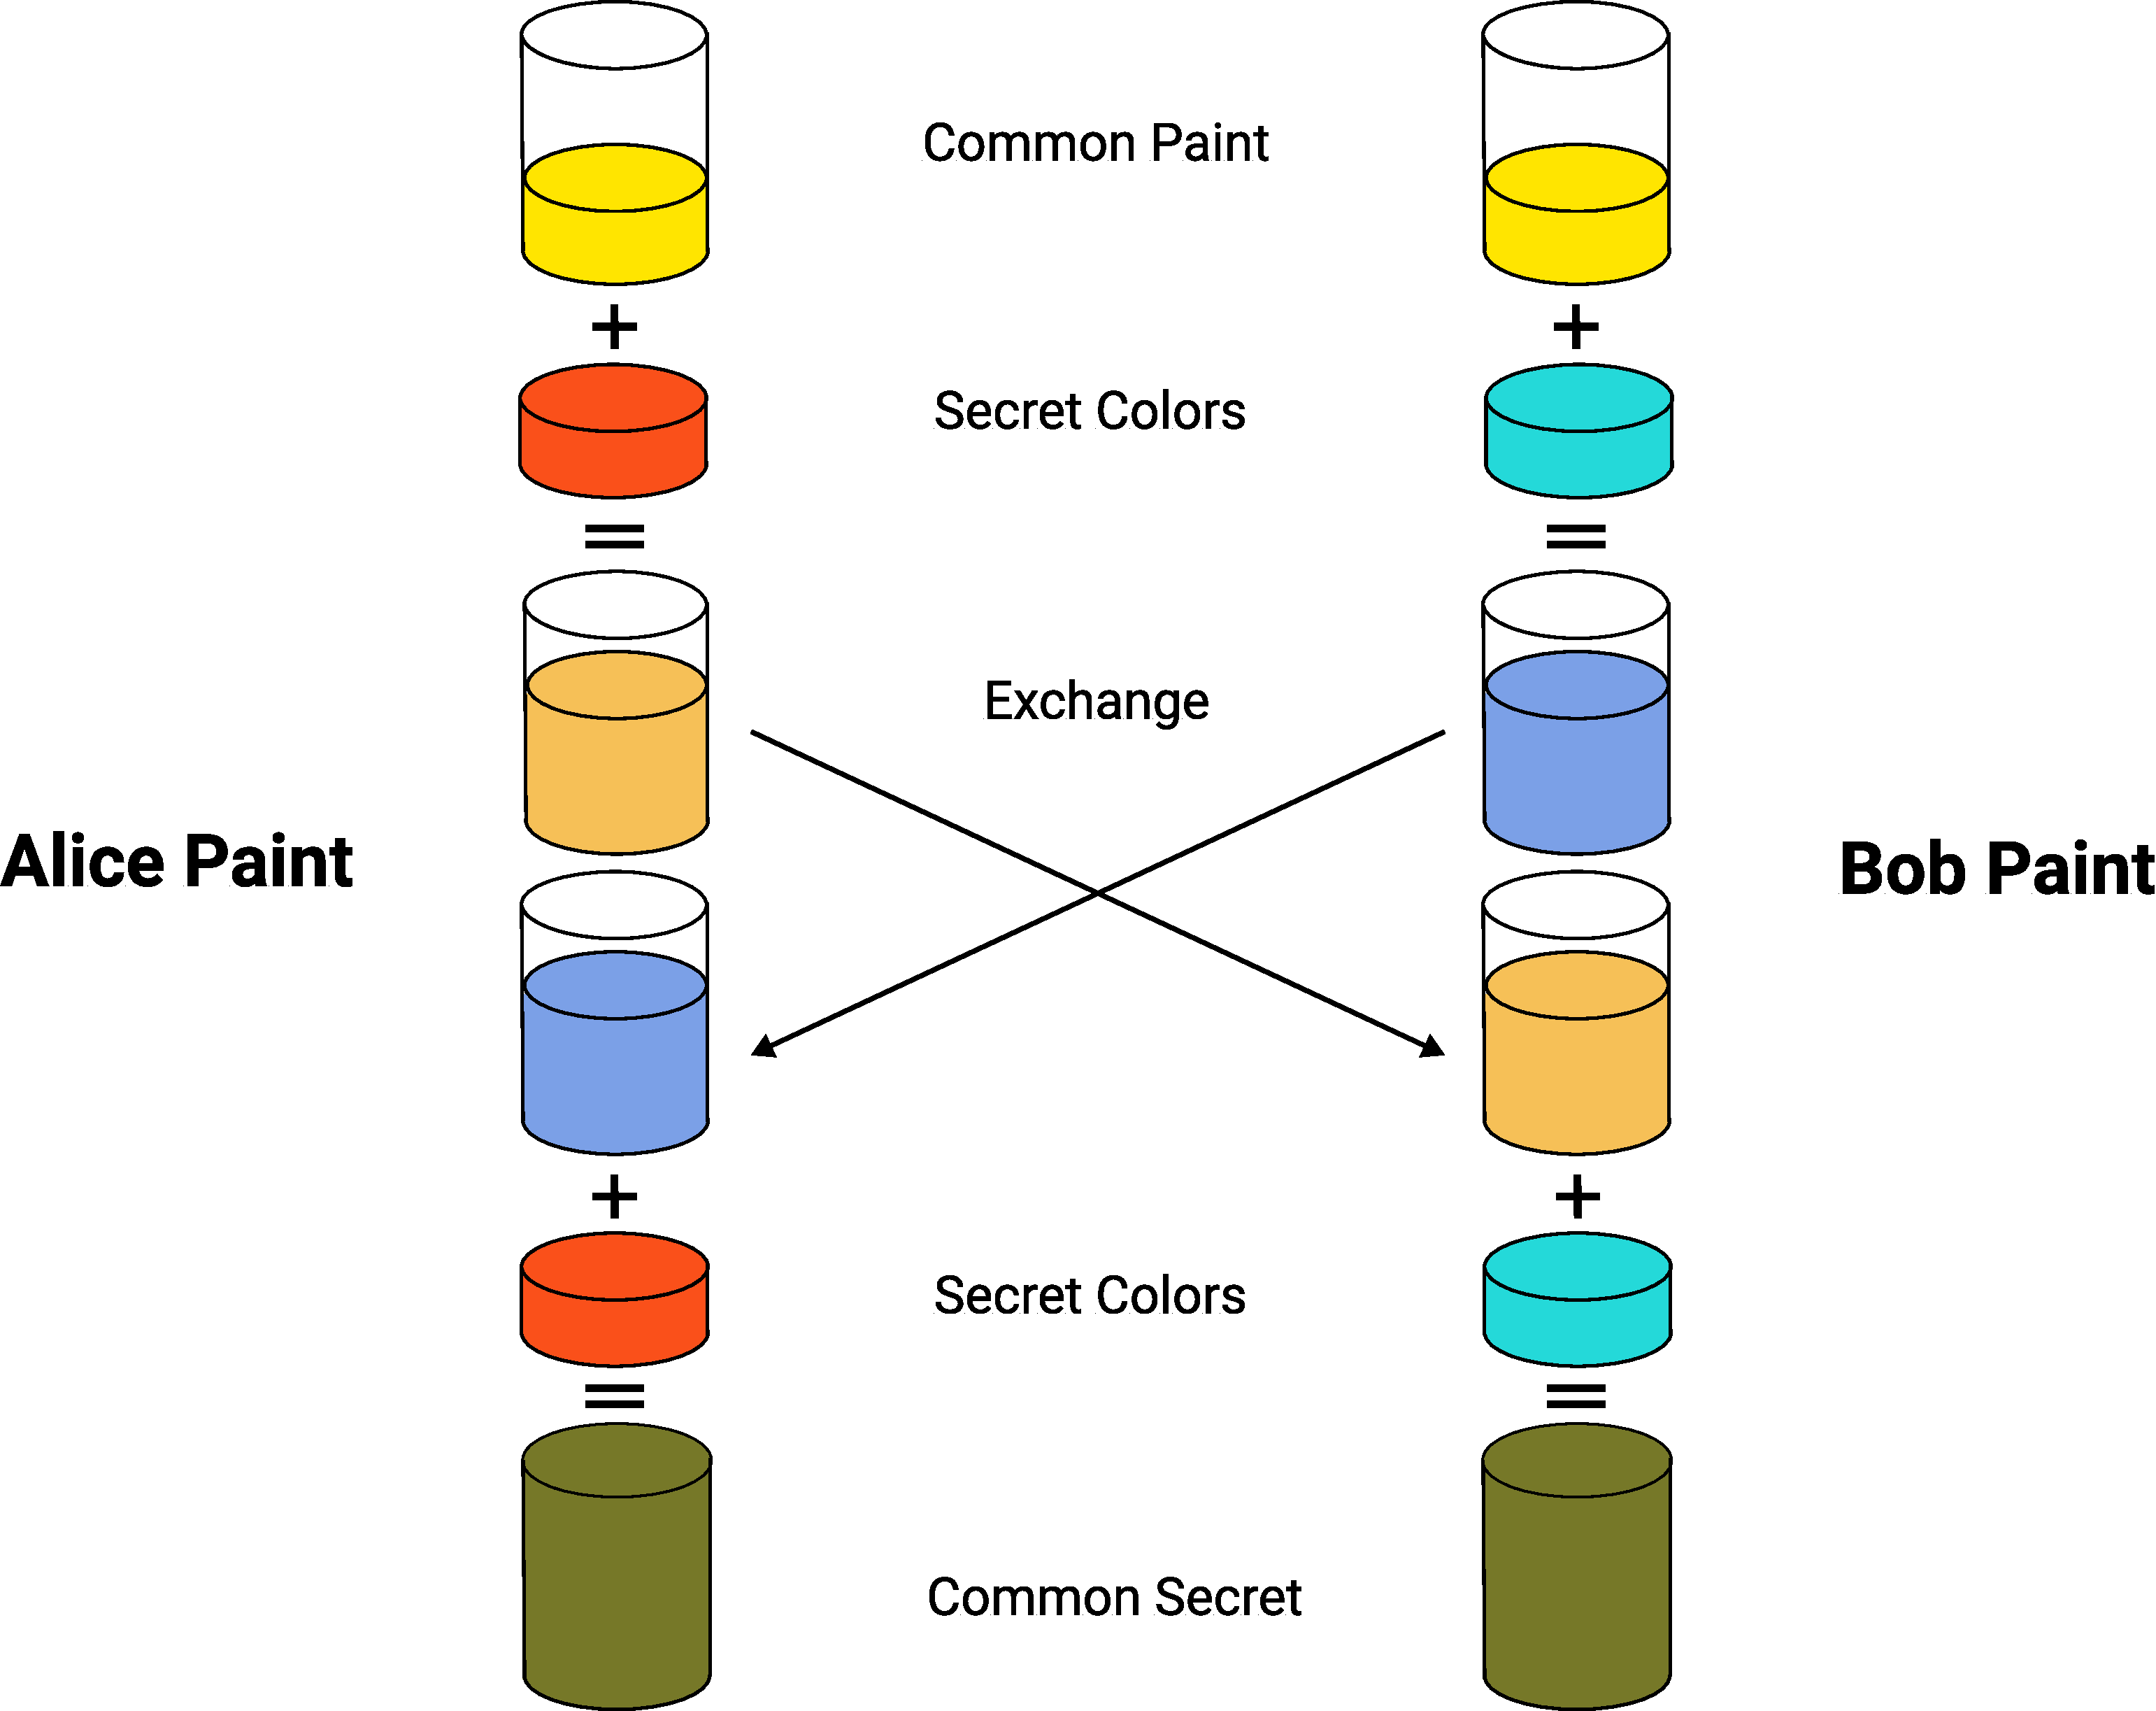
\includegraphics[width=1\textwidth]{Pictures/Diffie-Hellman}
    \caption{Illustration of the concept behind Diffie–Hellman key exchange. Source: }\label{fig:figure4}
\end{figure}
The process begins by having the two parties, Alice and Bob, publicly agree on an arbitrary starting color that does
not need to be kept secret (but should be different every time).
In this example, the color is yellow.
Each person also selects a secret color that they keep to themselves – in this case, red and blue-green.
The crucial part of the process is that Alice and Bob each mix their own secret color together with their mutually
shared color, resulting in orange-tan and light-blue mixtures respectively, and then publicly exchange the two mixed colors.
Finally, each of them mixes the color they received from the partner with their own private color.
The result is a final color mixture (yellow-brown in this case) that is identical to the partner's final color mixture.
If a third party listened to the exchange, it would only know the common color (yellow) and the first mixed colors
(orange-tan and light-blue), but it would be difficult for this party to determine the final secret color (yellow-brown).
Bringing the analogy back to a real-life exchange using large numbers rather than colors, this determination is
computationally expensive.
It is impossible to compute in a practical amount of time even for modern supercomputers.

The simplest and the original implementation of the protocol uses the multiplicative group of integers modulo $P$,
where $P$ is prime, and the generator $G$ which is a primitive root modulo $P$.
These two values are chosen in this way to ensure that the resulting shared secret can take on any value from $1$ to $P-1$.
Here is an example of the protocol
\begin{enumerate}
    \item Given modulus $P$ and generator $G$.
    \item Alice chooses her secret $a$.
    \item Alice sends to Bob $A, \; A = G^a \bmod P$.
    \item Bob chooses his secret $b$.
    \item Bob sends to Alice $B, \; B = G^b \bmod P$.
    \item Alice computes common secret $s, \; s = B^a \bmod P = (G^b \bmod P)^a \bmod P$.
    \item Bob computes common secret $s, \; s = A^b \bmod P = (G^a \bmod P)^b \bmod P$.
    \item Alice and Bob have arrived to the same value
    \[
        A^b \bmod P = G^{ab} \bmod P = G^{ba} \bmod P = B^a \bmod P,
    \]
    more specially,
    \[
        (G^a \bmod P)^b \bmod P = (G^b \bmod P)^a
    \]
\end{enumerate}
However, to reach a satisfactory level of security through DH key exchange a few rules have to be satisfied.
More precisely, Diffie-Hellman works in a multiplicative subgroup of integers modulo a given prime $p$.
To do some DH, you use some DH parameters which are:
\begin{itemize}
    \item p -- a big prime, called the "modulus"
    \item q -- a divisor of $p-1$, called the "subgroup order".
    \item g -- an integer modulo $p$ of order $q$, this means that the smallest integer $k > 0$ such that
    $g^k = 1 \bmod p$ is $k = q$.
\end{itemize}
For DH to be safe, you need the following:

\begin{itemize}
    \item Prime $p$ must defeat attempt at discrete logarithm through Index Calculus.
    This means that $p$ must be large enough, and also must not have any "special structure"
    such as being very close to a power of 2, because such structures allow for improvements in Index Calculus.
    It so happens that size requirements for DH are about the same as the size requirements for RSA,
    though the underlying reason for that is intricate and partly coincidental.
    So, basically, use a random $p$ of 2048 bits, and you will be fine.
    \item Number $q$ should be prime or have a prime divisor whose size is enough to defeat generic algorithms for
    discrete logarithm.
    If the size (in bits) of the largest prime divisor of $q$ is $z$, then generic algorithms have a cost in $2^{z/2}$.
    For best results, arrange for $q$ to be a prime of 256 bits or more.
    \item Systems that use the parameters to perform a DH key exchange must generate a random integer
    between $1$ and $q-1$ uniformly, using a cryptographically strong source of randomness, of course.
    If $q$ is prime and larger than 256 bits, it suffices to choose a 256-bit random value
    to achieve 128-bit of security.
    However, if $q$ is not prime, things are more complex: if $q$ has size $r$ bits,
    and the largest prime divisor of $q$ has size $e$ bits, and $e \geq 256$,
    then one may choose a random value $x$ of size $r-(e-256)$
    bits to get the usual "128-bit security".
    \item When $p$ is a so-called "safe prime", then $p = 2r+1$ for a prime $r$, so for any generator $g$ that is
    not $1$ or $p-1$, the order of $g$ will be either $r$ or $2r$, so it suffices to generate DH secret keys
    $x$ as random 257-bit values.
    The "safe primes" are not actually any safer than other primes,
    except for that point: they tolerate the choice of relatively small DH secret keys for any generator.
    \item Last but not least, DH is a key exchange algorithm that does not,
    inherently, provide authentication or confidentiality.
    DH is "safe" only when used within a protocol that uses DH and other algorithms with proper
    integration to achieve such sought after characteristics as data confidentiality and integrity.
\end{itemize}

Speaking of which, some (many) SSL/TLS implementations did things improperly, in that they
gladly accepted to do DH with weak parameters, in particular a 512-bit modulus.
The protocol itself is suboptimal in its handling of DH because the \texttt{ServerKeyExchange}
message allows the server to send the DH parameters $p$ and $g$ to the client, but not $q$,
leaving the client a bit in the dark.
Thus, the client must either "play safe" and generate its key in the full $1, \;\dots,\; p-1$ range,
or try to use a shorter exponent (say, 256 bits, not 2048) for a reduced computational cost,
but possibly at risk of weakness in case the subgroup order $q$ is not prime.
A better design would have allowed the server to send the value of $q$ and the size of the
biggest prime divisor of $q$.
In that respect, the ECDHE cipher suites of SSL/TLS (DH translated to elliptic curves)
have a better design.

For a practical answer if you are configuring your SSL/TLS server:
you should use a modulus of at least 2048-bit, and a generator $g$ such that the order
of $g$ is a prime $q$ of at least 256 bits;
alternatively, you may use a modulus $p$ which
is a "safe prime", the order of $g$ will then be either a very big prime, or twice
a very big prime, which is almost as good.
Some people feel safer when they generate their DH parameters
"themselves" instead of reusing existing values;
if that's what it takes
to allow you to sleep at night, then do it.

%\subsection{Secrecy Chart}\label{subsec:secrecy-chart}
%The chart below depicts who knows what, again with non-secret values in \textcolor{blue}{blue}, and secret values in \textcolor{red}{red}.
%Here Eve is an eavesdropper – she watches what is sent between Alice and Bob, but she does not alter the contents of their communications.
%\begin{itemize}
%    \item \textcolor{blue}{g} = public (prime) base, known to Alice, Bob, and Eve. $\textcolor{blue}{g = 5}$
%    \item \textcolor{blue}{p} = public (prime) modulus, known to Alice, Bob, and Eve. $\textcolor{blue}{p = 23}$
%    \item \textcolor{red}{a} = Alice's private key, known only to Alice. $\textcolor{red}{a = 6}$
%    \item \textcolor{red}{b} = Bob's private key known only to Bob. $\textcolor{red}{b = 15}$
%    \item \textcolor{blue}{A} = Alice's public key, known to Alice, Bob, and Eve. $\textcolor{blue}{A = g}^{\textcolor{red}{a}} \, mod \, \textcolor{blue}{p = 8}$
%    \item \textcolor{blue}{B} = Bob's public key, known to Alice, Bob, and Eve. $\textcolor{blue}{B = g}^{\textcolor{red}{a}} \, mod \, \textcolor{blue}{p = 8}$
%\end{itemize}
%\begin{center}
%    \begin{table}
%        \begin{tabular}{|c|c|c|c|c|c|}
%            \hline
%            \multicolumn{2}{|c|}{Alice} & \multicolumn{2}{c|}{Bob} & \multicolumn{2}{c|}{Eve}
%            \cr \hline
%            known & unknown & known & unknown & known & unknown
%            \cr \hline
%            $\textcolor{blue}{p = 23}$ & & $\textcolor{blue}{p = 23}$  & & $\textcolor{blue}{p = 23}$ &
%            \cr \hline
%            $\textcolor{blue}{g = 5}$ & & $\textcolor{blue}{g = 5}$ & & $\textcolor{blue}{g = 5}$ &
%            \cr \hline
%            $\textcolor{red}{a = 6}$ & $\textcolor{red}{b}$ & $\textcolor{red}{b = 15}$ & $\textcolor{red}{a}$ & & $\textcolor{red}{a, b}$
%            \cr \hline
%            $\textcolor{blue}{A = 5}^{\textcolor{red}{a}} \, mod \, \textcolor{blue}{23}$ & & $\textcolor{blue}{B = 5}^{\textcolor{red}{b}} \, mod \, \textcolor{blue}{23}$ & & &
%            \cr \hline
%            $\textcolor{blue}{A = 5}^{\textcolor{red}{6}} \, mod \, \textcolor{blue}{23} = \textcolor{blue}{8}$ & & $\textcolor{blue}{B = 5}^{\textcolor{red}{15}} \, mod \, \textcolor{blue}{23} = \textcolor{blue}{19}$ & & &
%            \cr \hline
%            $\textbf{\textcolor{blue}{B}} = \textbf{\textcolor{blue}{19}}$ & & $\textbf{\textcolor{blue}{A}} = \textbf{\textcolor{blue}{8}}$ & & $\textcolor{blue}{A} = \textcolor{blue}{8}$, $\textcolor{blue}{B} = \textcolor{blue}{19}$ &
%            \cr \hline
%            $\textbf{\textcolor{red}{s}} = \textcolor{blue}{B}^{\textcolor{red}{a}} \, mod \, \textcolor{blue}{23}$ & & $\textbf{\textcolor{red}{s}} = \textcolor{blue}{A}^{\textcolor{red}{b}} \, mod \, \textcolor{blue}{23}$ & & &
%            \cr \hline
%            $\textbf{\textcolor{red}{s}} = \textcolor{blue}{19}^{\textcolor{red}{6}} \, mod \, \textcolor{blue}{23} = \textcolor{red}{2}$ & & $\textbf{\textcolor{red}{s}} = \textcolor{blue}{A}^{\textcolor{red}{b}} \, mod \, \textcolor{blue}{23} = \textcolor{red}{2}$ & & &
%            \cr \hline
%
%        \end{tabular}
%        \label{tab:table}
%    \end{table}
%\end{center}
%Now \textcolor{red}{s} is the shared secret key and it is known to both Alice and Bob, but not to Eve.
%Note that it is not helpful for Eve to compute \textcolor{blue}{AB}, which equals
%$\textcolor{blue}{g}^{\textcolor{red}{a} + \textcolor{red}{b}} \, mod \, \textcolor{blue}{p}$.
%Note that it should be difficult for Alice to solve for Bob's private key or for Bob to solve for Alice's private key.
%If it is not difficult for Alice to solve for Bob's private key (or vice versa), Eve may simply substitute her own
%private / public key pair, plug Bob's public key into her private key, produce a fake shared secret key, and solve for
%Bob's private key (and use that to solve for the shared secret key.
%Eve may attempt to choose a public / private key pair that will make it easy for her to solve for Bob's private key).

\begin{figure}[H]
    \centering
    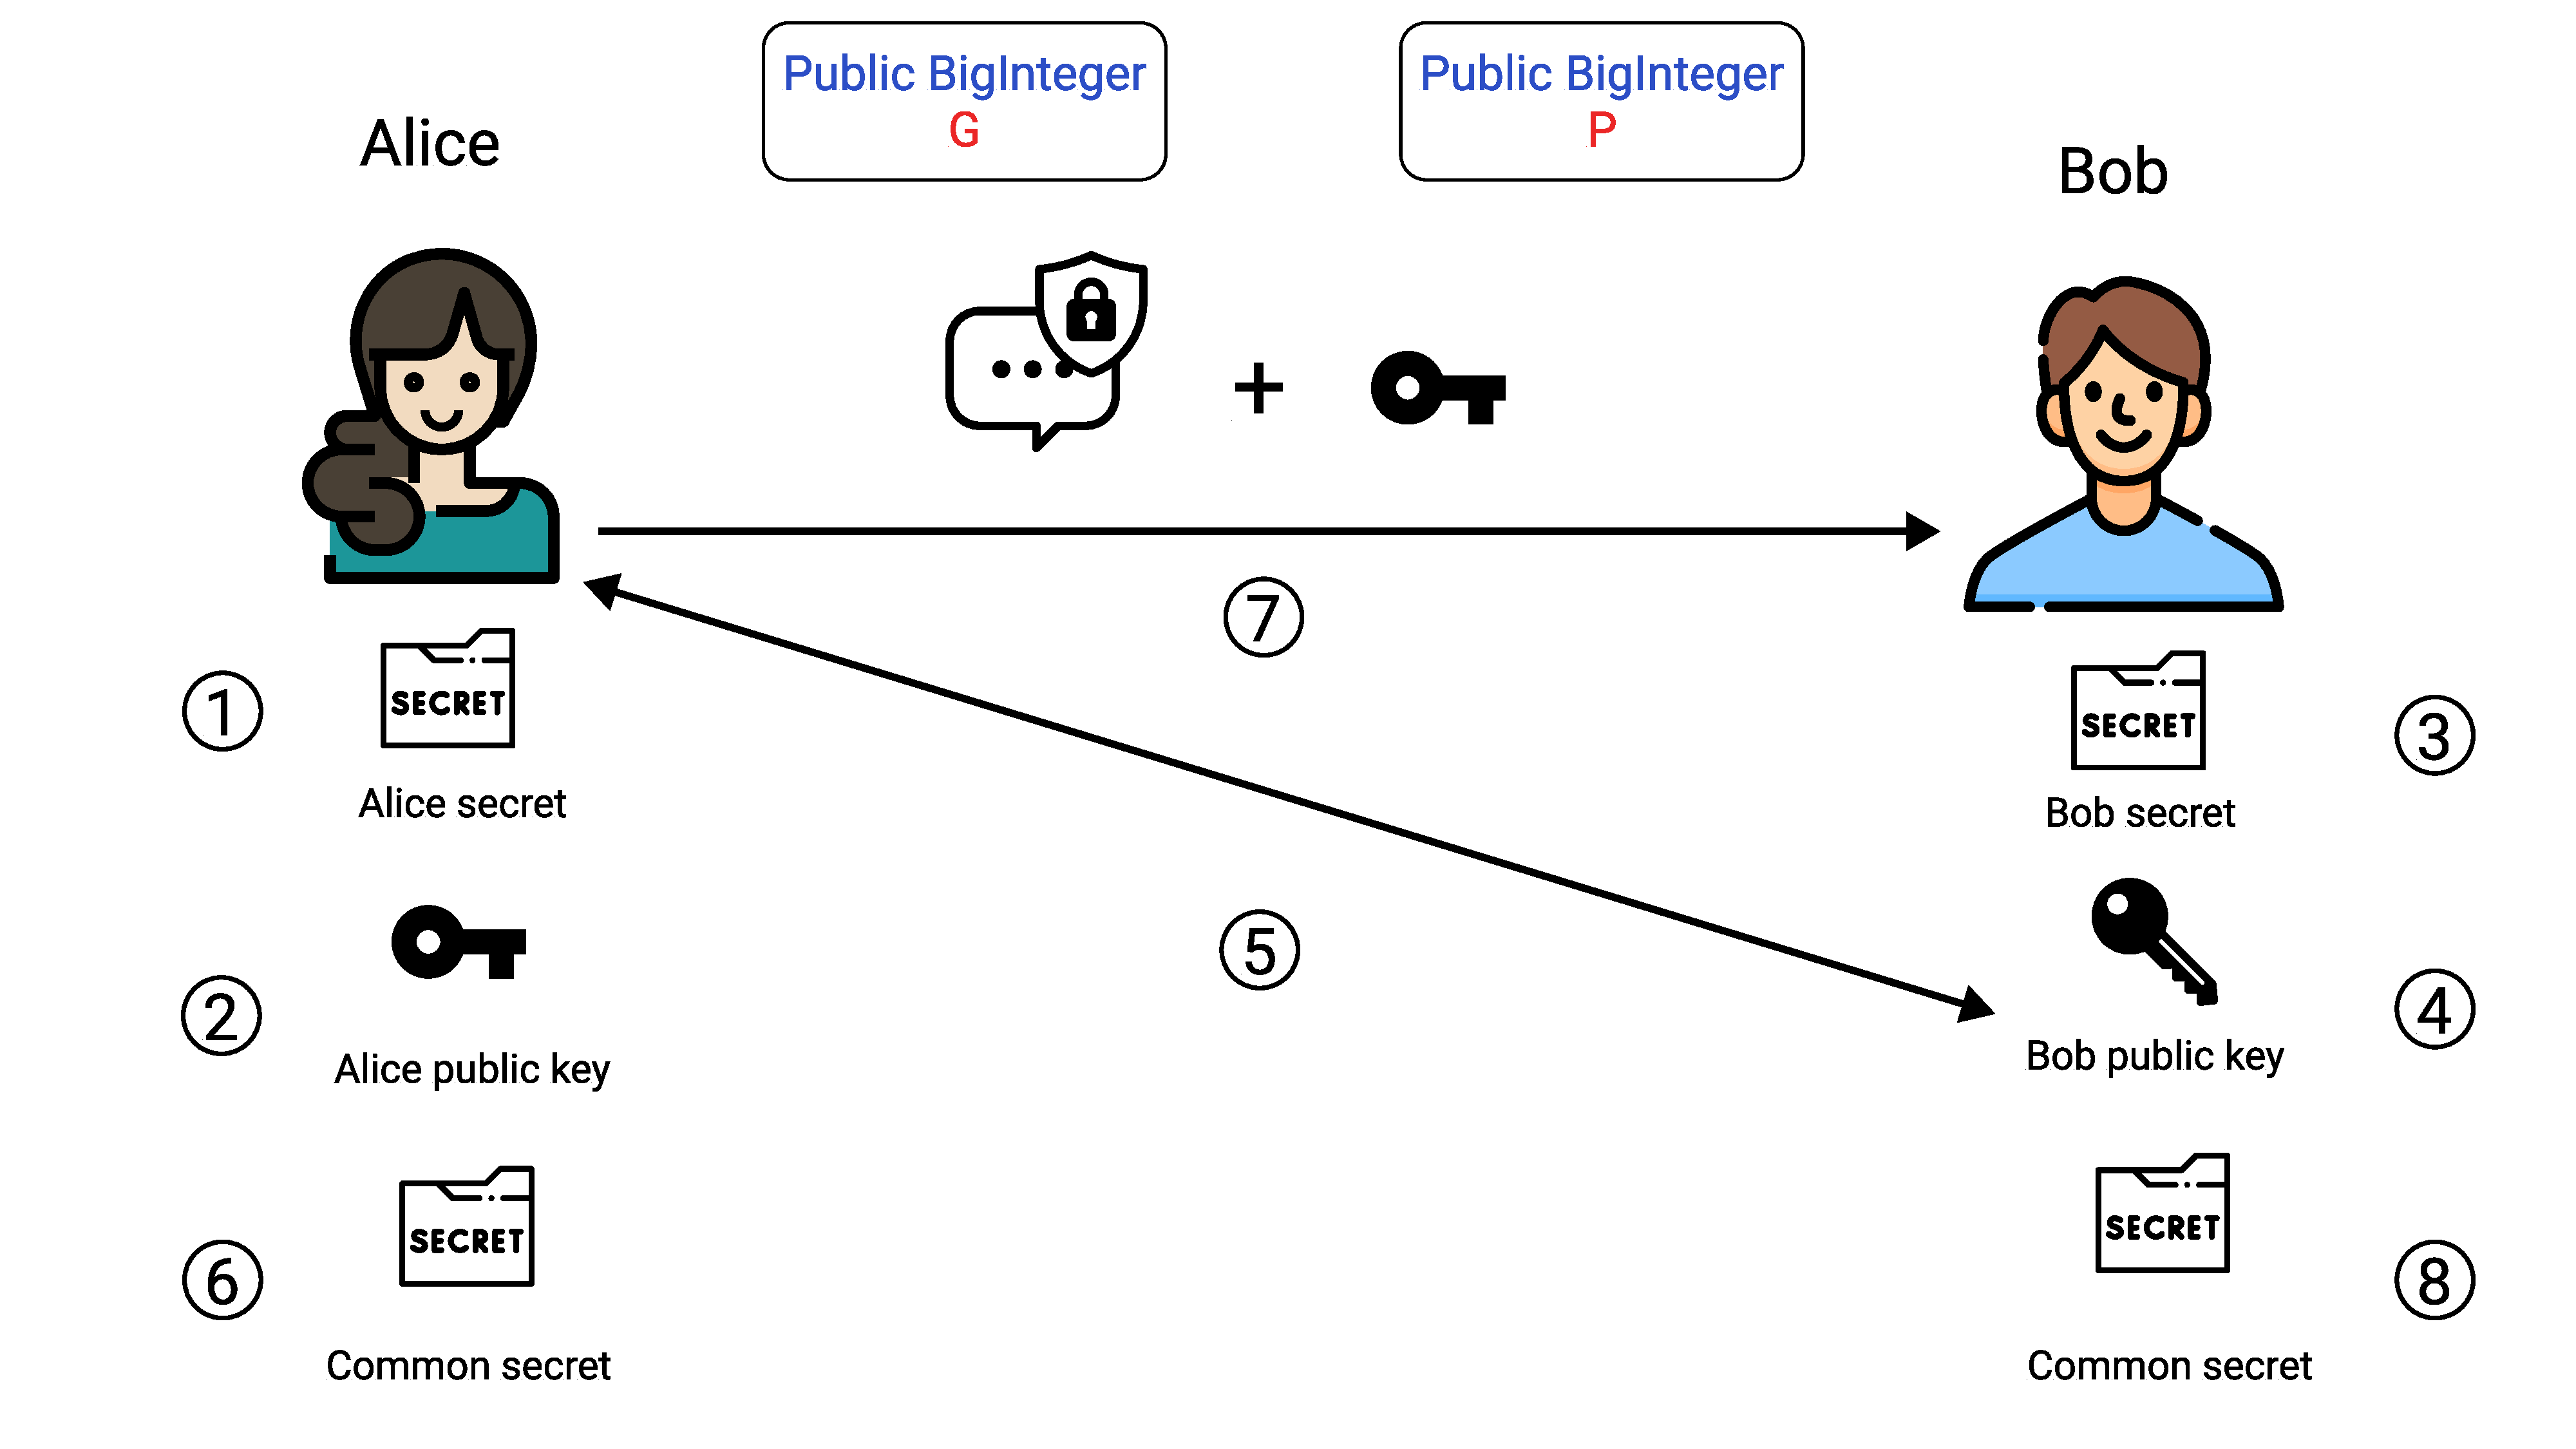
\includegraphics[width=1\textwidth]{Pictures/Key_Exchange}
    \caption{Secret chat encryption concept diagram. Source: }\label{fig:figure7}
\end{figure}
Assume that Alice wants to write a secret message to the Bob.
The secret chat encryption implemented as follows
\begin{enumerate}
    \item Given two public constants: $P, G$.
    \item Alice generates her secret $a$.
    \item Alice generates public key $A$ as $A=G^a \bmod P$ and shares it public.
    \item Bob generates his secret $b$.
    \item Bob generates public key $B$ as $B=G^b \bmod P$ and shares it public.
    \item Alice reads Bob's public key $B$.
    \item Alice calculates Common secret $s$ as $s = B^a \bmod P$.
    \item Alice encrypts message using AES256 algorithm, then sends it to Bob along her public key $A$.
    \item Bob calculates Common secret $s$ as $s = A^b \bmod P$ and decrypts message from Alice.
\end{enumerate}
Although, DH fits the key exchange concerns fine, the secret might be shared via RSA approach as well.
We discuss it in next section.

%----------------------------------------------------------------------------------------
%	BIBLIOGRAPHY
%----------------------------------------------------------------------------------------

    \printbibliography[heading=bibintoc]

%----------------------------------------------------------------------------------------

%----------------------------------------------------------------------------------------
%	THESIS CONTENT - APPENDICES
%----------------------------------------------------------------------------------------

    \appendix % Cue to tell LaTeX that the following "chapters" are Appendices

% Include the appendices of the thesis as separate files from the Appendices folder
% Uncomment the lines as you write the Appendices

    \chapter{List of functional requirements}\label{ch:list-of-functional-requirements}
\textbf{Registration user stories}
\begin{itemize}
    \item As an unregistered user, I want to tap “Register” so that I see the registration form and register myself.
    \item As an unregistered user, I want to use my phone number to register so that my account is tied to my phone number.
    \item As an unregistered user, I want to use my e-mail address to register so that my account is tied to my e-mail address.
    \item As an unregistered user, I want to add a display name during registration so that other users can find me using it.
    \item As an unregistered user, I want to choose how to receive the registration confirmation via SMS or e-mail so that
    notification is sent to me via SMS or e-email.
    \item As an unregistered user, I want to receive the registration confirmation via SMS or Email so that I can activate my account.
    \item As a registered user, I want to confirm my email address so that I get confirmation link via email I provided.
    \item As a registered user, I want to confirm my phone number so that I use specified form to do it.
\end{itemize}

\textbf{Authentication user stories}
\begin{itemize}
    \item As a registered user, I want to authenticate myself using both combinations email-password and phone-password
    so that I use the specified form with two inputs.
    \item As a registered user, I want to restore my password if I forget it so that I use specified form and restore my password.
    \item As an authenticated user, I want my session on each device to least 7 days so that after 7 days of inactivity device
    will be logged out automatically.
\end{itemize}

\textbf{Managing contacts user stories}
\begin{itemize}
    \item As an authorized user, I want to see my contact list so that there is a list of users who are my contacts.
    \item As an authorized user, I want to search users so that I write user display name or phone number of e-mail
    address to specified input, click "Search user" button and see results.
    \item As an authorized user, I want to add other user to my contact list so that I click "Add contact" button on
    user profile and add him to my contact list.
    \item As an authorized user, I want user search input to accept empty or whitespace queries so that all users
    displayed as search result.
    \item As an authorized user, I want to remove the user from my contact list so that I click "Remove contact" button
    on user profile and remove him from my contact list.
    \item As an authorized user, I want to navigate to private chat with the user from my contact list so that I click
    "Message" button at user profile and get navigated to the private chat with him.
    \item As an authorized user, I want to tap "Start chat" so that create chat with specified user/contact
\end{itemize}

\textbf{Sending messages and media to individuals user stories}
\begin{itemize}
    \item As an authorized user, I want to send a text message so that another user sees my message.
    \item As an authorized user, I want to add an attachment to the message so that another user sees the message with attachment.
    \item As an authorized user, I want to add an emoji to the message so that another user sees the message with emoji.
    \item As an authorized user, I want to tap "Edit" on my message so that message I edited is changed immediately in the chat.
    \item As an authorized user, I want to tap "Delete" on my message so that message immediately disappears from the chat.
    \item As an authorized user, I want to share secret messages with users from my contact list so that our are
    messages encrypted for anyone else including system administrators.
    \item As an authorized user, I want each new message in private chats I participate to be displayed immediately
    in real-time so that I do not reload page.
\end{itemize}

\textbf{Navigation user stories}
\begin{itemize}
    \item As an authorized user, I want to navigate between the pages so that there is a menu on the UI.
\end{itemize}

\textbf{Creating and managing groups user stories}
\begin{itemize}
    \item As a registered user, I want to tap "Create channel" so that I create a new channel of the one of the types:
    Private channel, Public channel, Readonly channel.
    \item As a registered user, I want to tap "Start direct chat" so that I create a new direct chat with specified user.
    \item As a registered user, I want to tap "Start secret chat" so that I create a new secret chat with specified user.
    \item As a registered user, I want to join public groups so that I click button "Join group" to join the group.
    \item As a registered user, I want to tap "Archive" so that I archive the specified chat or channel.
    \item As a registered user, I want to tap "Un-archive" so that I un-archive the specified archived chat or channel.
    \item As a registered user, I want my secret chats to be device-specific so that I can see a secret chat only
    on the device that I used to start this chat.
    \item As registered user, I want to tap "Leave" so that I leave from specified chat or channel.
\end{itemize}

\textbf{Sending messages and media to groups user stories}
\begin{itemize}
    \item As an authorized user, I want to send a text message so that other members of the group see the message I sent.
    \item As an authorized user, I want to add an attachment to the message so that other members of the group see the
    message with attachment I sent.
    \item As an authorized user, I want to add an emoji to the message so that other members of the group see the message with emoji I sent.
    \item As an authorized user, I want to tap "Edit" on my message so that other members of the group see the message I edited.
    \item As an authorized user, I want to tap "Delete" on my message so that my message is deleted for all members of the group.
    \item As an authorized user, I want to search public groups by title so that I enter display name to specified field,
    click button "Search chats" and see results.
    \item As an authorized user, I want each new message in groups I participate to be displayed immediately in
    real-time so that I do not reload page.
\end{itemize}

\textbf{Viewing messages history user stories}
\begin{itemize}
    \item As an authorized user, I want to view a message history of particular chat or group so that I see a list of
    my active chats on the UI\@.
    \item As an authorized user, I want to search messages in particular chat so that I see the results in messages
    window of the chat.
\end{itemize}

\textbf{Managing profile settings user stories}
\begin{itemize}
    \item As an authorized user, I want to update my personal information in profile settings so that other users my
    updated personal information.
    \item As an authorized user, I want to update my social network links in profile settings so that other users
    my updated social media.
    \item As an authorized user, I want to change my profile picture so that all other users will see updated one.
    \item As an authorized user, I want reset password, so that my password will change.
    \item As an authorized user, I want to tap "Logout" button so that current device will be logged out from the system.
    \item As an authorized user, I want to tap "Logout all" button so that all my authorized devices will be logged out
    from the system.
    \item As an authorized user, I want to navigate to personal information page so that I want see my profile picture.
    \item As an authorized user, I want to navigate to personal information page so that I want see my personal information.
    \item As an authorized user, I want to tap "Reset" so that I want reset my updated (not saved) personal information.
    \item As an authorized user, I want save my updated personal information so that users see it.
\end{itemize}
    \chapter*{List of non-functional requirements}\label{ch:list-of-non-functional-requirements}
\begin{itemize}
    \item Graphic user interface of the system should be well organized.
    To fulfill this requirement, we follow an ISO 9241--161:2010 (en) Ergonomics of human-system interaction
    standard [\cite{iso2010ergonomics}].
    \item The system should have well performance, which meant to respond it at least 1 second.
    User should have a device with at least 6 GB RAM and CPU with 1.8 GHZ, 100 Mbps internet connection.
    Server must have the following hardware: Intel 1+ GHz 2 Cores server processor, 2GB DDR4 memory, NVME or SAS
    server disk with a minimum capacity of 1.6 GB\@.
    \item The unique, unambiguous identifier of users in the system is the username.
    It is set in the profile settings.
    \item The Web UI must be well displayed with the following browsers, in the versions
    current at the date of receipt of the system or, depending on technical possibilities,
    with the latest versions that support correct operation of the system:
    \begin{itemize}
        \item Google Chrome 72.0.36.
        \item Mozilla Firefox 64.0.2.
        \item Microsoft Edge 17.17134.
    \end{itemize}
    \item The system shall force users to use passwords with a minimum length of 8
    characters and using at least one capital letter and one number and one special symbol.
    \item The Web UI must be compatible to use on mobile device screens with a minimum
    width of 600 pixels.
    \item The Web UI must be compatible to use on desktop or laptop device screens with a
    minimum display width of 1024 pixels.
\end{itemize}
    \chapter{RSA Algorithm comments}\label{ch:rsa-algorithm-comments}


\section{One way functions}\label{sec:one-way-functions}
One way function -- is a function that is easy to compute on every input, but
hard to invert given the image of a random input.
For instance, the function
\begin{equation*}
    f(m) = m^e \bmod N \equiv C
\end{equation*}
where $e, N$ are public constants is one-awy function,
because it is easy to compute $C$ given $m$, however it is hard to compute $m$ given $C$.


\section{Euler's totient theorem}\label{sec:euler's-totient-theorem}
Given a number $N$ and its prime factorization $p_1^{e_1}\cdot p_2^{e_2} \cdots p_k^{e_k}$, then Euler's totient function
$\phi(N)$ is defined as

\[
    \phi(N) = (p_1^{e_1} - p_1^{e_1 - 1}) \cdot (p_2^{e_2} - p_2^{e_2 - 1}) \cdots (p_k^{e_k} - p_k^{e_k - 1})
\]

In particular, for positive number $M$ such that its factorization is $p1 \cdot p2$, the $\phi(M)$ is

\[
    \phi(M) = (p_1 -1) \cdot (p_2 - 1)
\]

Euler's theorem relates the modular division and exponent as follows, given number $m$, then
\[
    m^{\phi(N)} = 1 \bmod N
\]
It means that reminder of division $m^{\phi(N)}$ by $N$ is always 1.
By the equality $1^K = 1$
\[
    M^{K \cdot \phi(N)} = 1 \bmod N
\]
If we multiply both parts by $M$, we get
\[
    M \cdot M^{K \cdot \phi(N)} = M^{K \cdot \phi(N) + 1} = M \bmod N
\]


%! suppress = TooLargeSection


\section{RSA Encryption algorithm}\label{sec:rsa-encryption-algorithm}
The RSA algorithm is named after Ron Rivest, Adi Shamir and Len Adleman, who invented it in 1977 [\cite{rivest1978method}].
The basic technique was first discovered in 1973 by Clifford Cocks [\cite{cocks1973note}] of CESG (part of the British GCHQ)
but this was a secret until 1997.
The patent taken out by RSA Labs has expired.

Historically, the process of encryption is considered to be symmetric one.
That means that prior the communication, the sides conclude on the common key to be used in encryption.
This process is similar to the first sharing keys and only after that the locked chest with the message.
Such approach is highly cost since it requires to share the defined keys between each actor if the number of actors
is greater than 2.
Much more simpler is to think about secured communication channel that in terms of asymmetric encryption.
The real life example would be if Alice shares with all actors an opened lock having key.
So that Bob receives an opened lock, writes letter to Alice, puts letter to the chest, locks this chest with received
from Alice lock.
This way, only Alice will be able to open the chest and to read the letter.
This is an idea of the asymmetric encryption.
However, such a simple from first glance idea requires complex number theory approach.
A concept of opened lock may be interpreted in terms of one-way functions.
One way function -- is a function that is easy to compute on every input, but hard to invert given the image of
a random input.
Thus, it is much simpler to close the lock without key, but very difficult to open lock trying the combinations
of the key.
For instance, the function
\begin{equation*}
    f(m) = m^e \bmod N = C
\end{equation*}
where $e, N$ are public constants is one-awy function,
because it is easy to compute $C$ given $m$, however it is hard to compute $m$ given $C$.
So, assume that Alice defines two positive integer constants $e, N$ and sends it to Bob.
Bob encrypts the secret message $m$ using $f(m)$
\[
    f(m) = m^e \bmod N = C
\]
Then Bob sends encrypted message $C$ to the Alice.
Given $C$ Alice must fetch the Bob's message $m$.
In order to decrypt $C$, Alice has to compute
\[
    C^d \bmod N = m^{ed} \bmod N \equiv m,
\]
where $e$ for encryption and $d$ for decryption.
Now the problem is to define such $d$ that it is hard to the listener to fetch it.
In order to define the secret $d$, Alice chooses two enough big prime numbers: $P, \; Q$, let's say around 150 digits
both.
Then Alice multiplies these two prime numbers in order to get $N$
\[
    N = P \cdot Q
\]
The $N$ is around 300 digits.
Now Alice can share $N$ with anyone, since it takes decades to find its prime factorization by the fundamental problem
of prime factorization.
Next, it is very important to know such a function, which depends on the knowledge of factorization of $N$.
Such function is an Euler's totient function.
Given a number $N$ and its prime factorization $p_1^{e_1}\cdot p_2^{e_2} \cdots p_k^{e_k}$, the Euler's totient function
$\phi(N)$ is defined as
\[
    \phi(N) = (p_1^{e_1} - p_1^{e_1 - 1}) \cdot (p_2^{e_2} - p_2^{e_2 - 1}) \cdots (p_k^{e_k} - p_k^{e_k - 1})
\]
In particular, for positive number $M$ such that its factorization is $p1 \cdot p2$, the $\phi(M)$ is
\[
    \phi(M) = (p_1 -1) \cdot (p_2 - 1)
\]
Euler's theorem relates the modular division and exponent as follows, given number $m$, then
\[
    m^{\phi(N)} = 1 \bmod N
\]
It means that reminder of division $m^{\phi(N)}$ by $N$ is always 1.
By the equality $1^K = 1$
\[
    M^{K \cdot \phi(N)} = 1 \bmod N
\]
If we multiply both parts by $M$, we get
\[
    M \cdot M^{K \cdot \phi(N)} = M^{K \cdot \phi(N) + 1} = M \bmod N
\]
It follows that Alice is able to define the secret $d$ as follows
\begin{gather*}
    e \cdot d = K \cdot \phi(N) + 1\\
    d = \frac{K \cdot \phi(N) + 1}{e}\\
\end{gather*}
The following image demonstrates the concept of RSA approach
\begin{figure}[H]
    \centering
    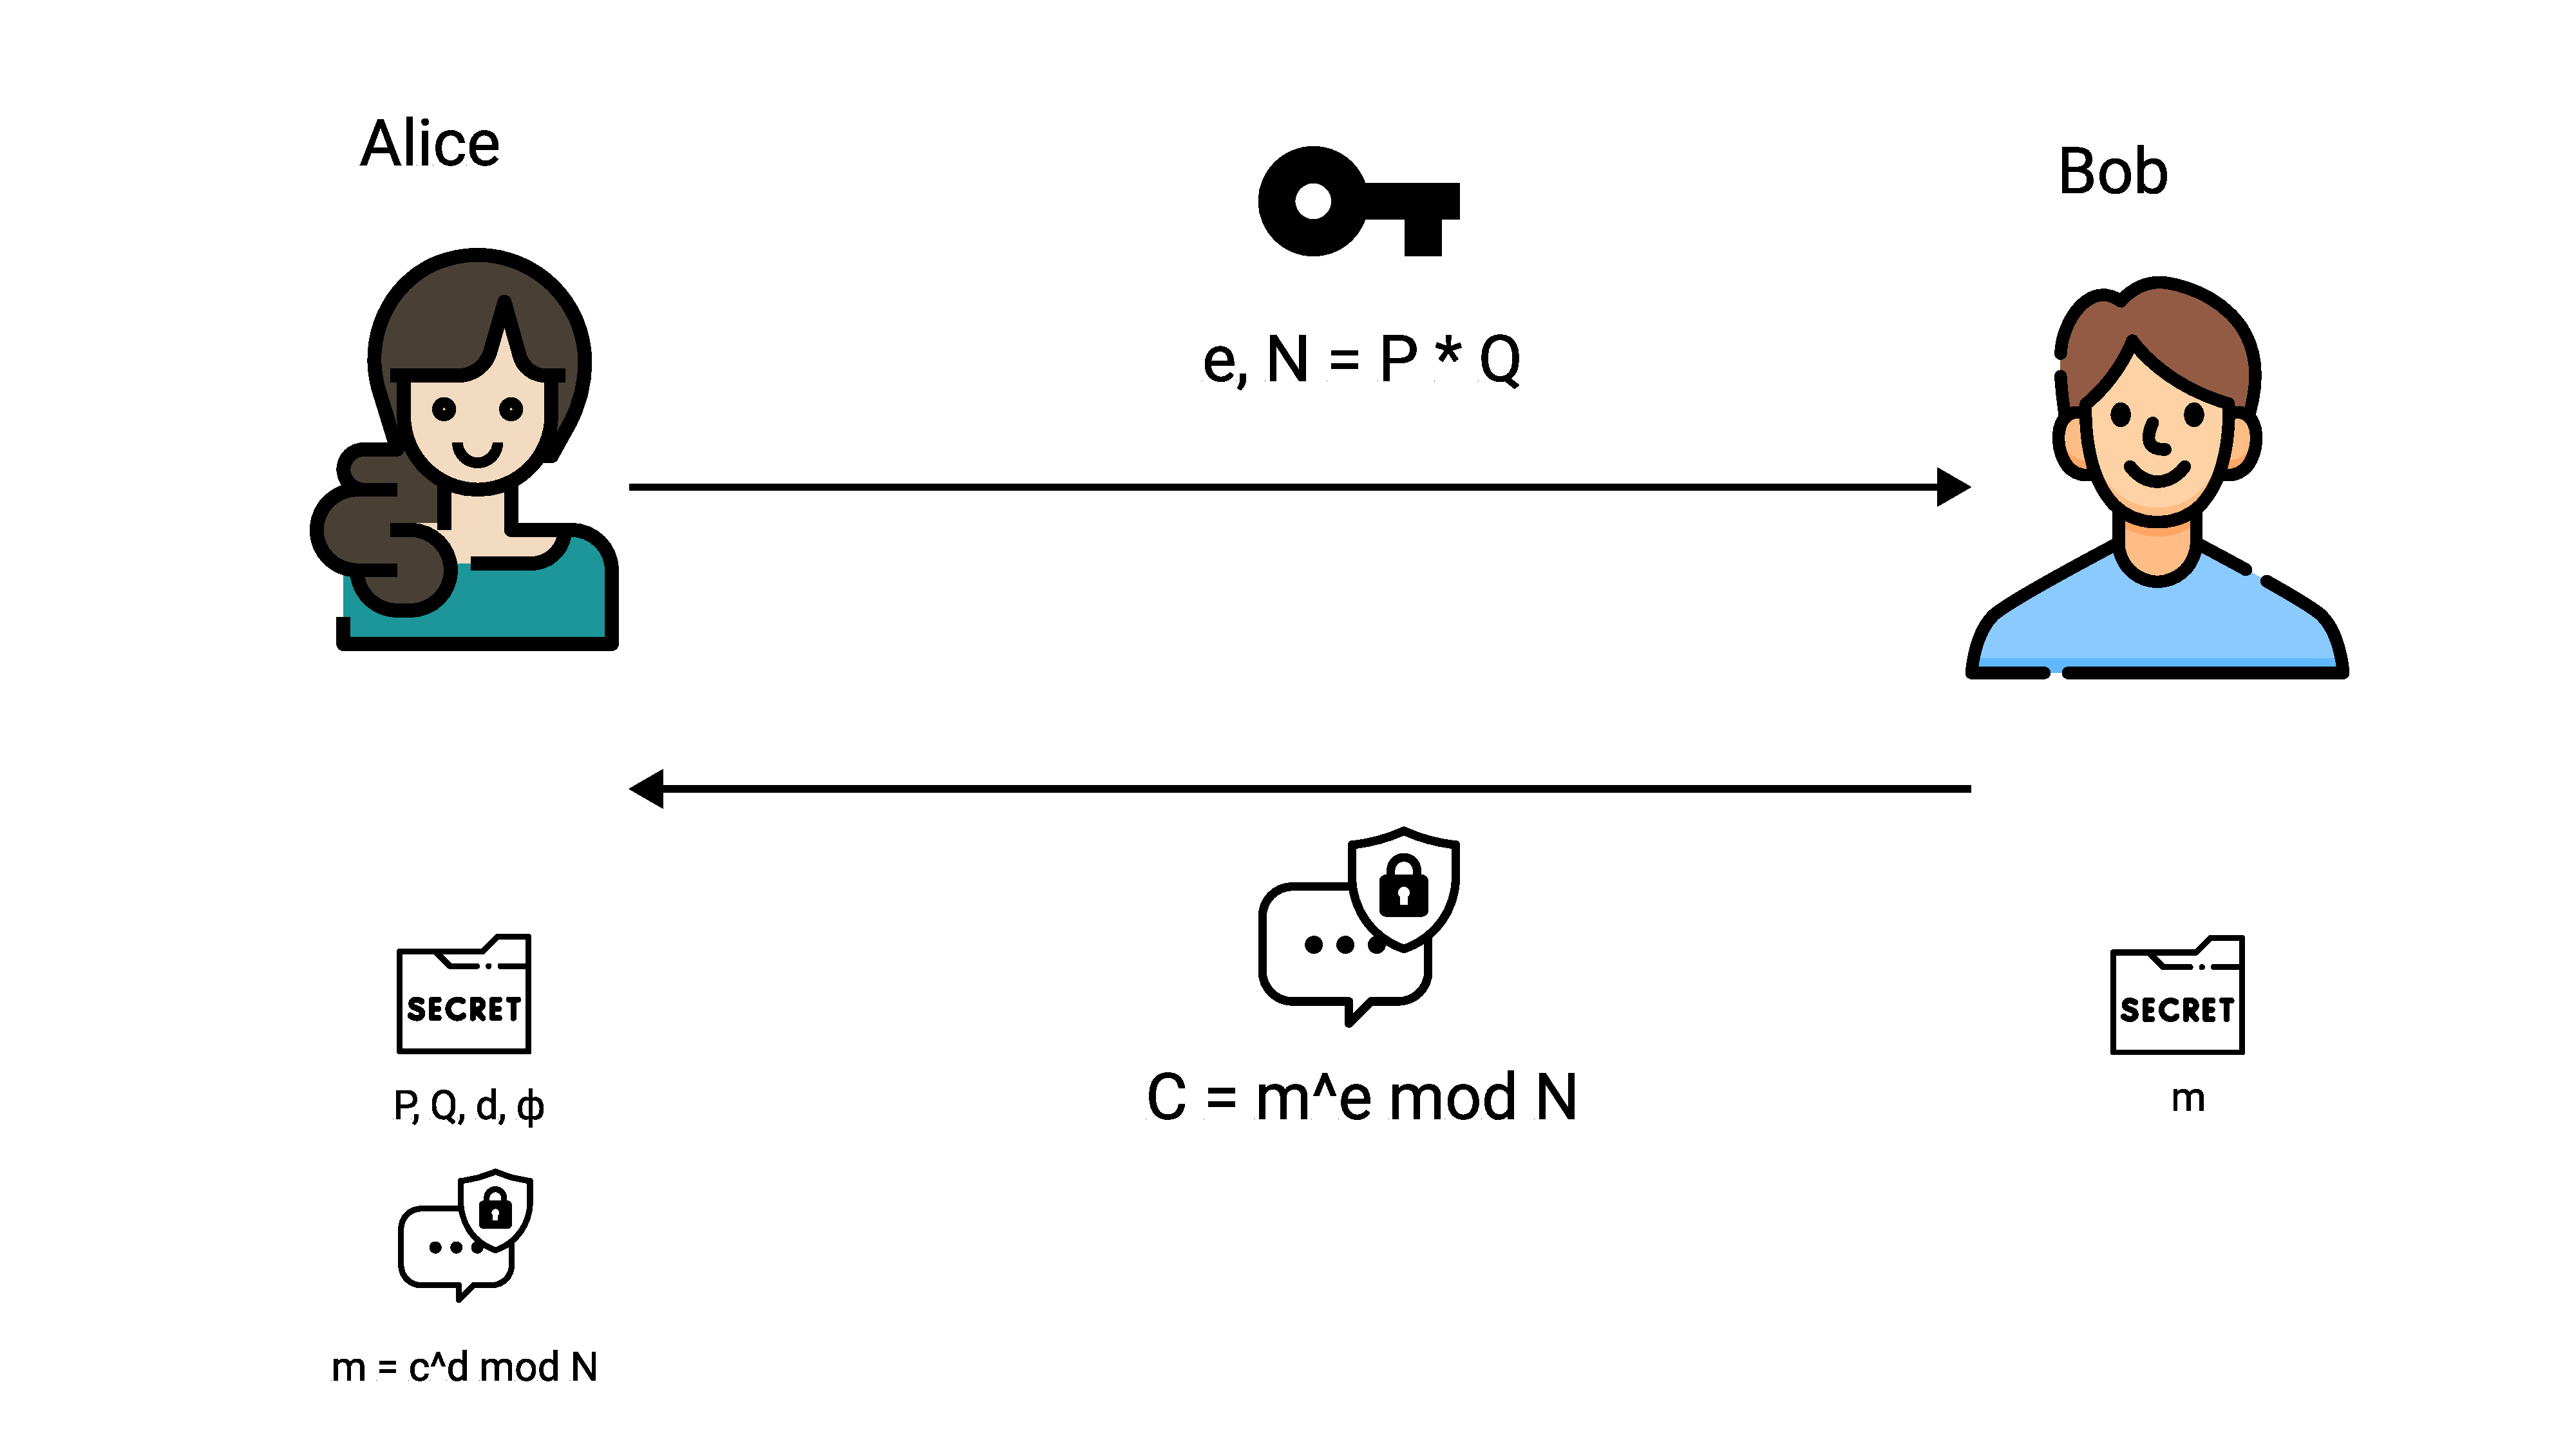
\includegraphics[width=1\textwidth]{Pictures/12_RSA_encryption_concept_diagram}
    \caption{RSA algorithm concept diagram. Source: }\label{fig:figure8}
\end{figure}
To summarize, the process by the steps is as follows
\begin{itemize}
    \item Alice defines the large secret prime numbers $P, \; Q$.
    \item Alice computes $N = P \cdot Q$ and $\phi = (P-1)(Q-1)$
    \item Alice chooses an integer $e$, $1<e< \phi$ such that $\gcd(e, \phi) = 1$.
    \item Alice computes secret exponent $d$, $1<d< \phi$ such that $ed \equiv 1 \bmod \phi$.
    \item Alice shares public key $(N,e)$ with Bob and keeps private key $(d, p, q)$ is secret.
    \item Bob defines the message $m$, encrypts it as $C = m^{e} \bmod N$.
    \item Bob sends $C$ to Alice.
    \item Alice decrypts $C$ using her secret $d$, so she gets $m$
    \[
        m = C^d \bmod N
    \]
\end{itemize}
Security of the RSA approach is based on the complexity of fundamental problem of prime factorization,
which takes decades to solve having enough large number.
%    \chapter{Azure deployment via GitHub Actions}\label{ch:azure-deloyment-via-github-actions}
In this attachment deployment process to Azure via GitHub pages is described.


\section{Creating Database}\label{sec:creating-database}


\section{Setting up Azure Virtual Machine}\label{sec:setting-up-azure-environment}
As for student, Azure offers a lot of 100USD limited "free" opportunities,
provided that we won't pay in the future.
We require only a few things: Ubuntu based virtual machine, database, static IP address.
Azure provides such discounts for the
\begin{itemize}
    \item Virtual machine \texttt{Standard B1s (1 vcpu, 1 GiB memory)}
    \item Database \texttt{Burstable, B1ms, 1 vCores, 2 GiB RAM, 32 GiB storage}
\end{itemize}
And that's enough for our purposes.
Approximate cost per month for \texttt{Standard B1s (1 vcpu, 1 GiB memory)} is 8,25 USD/month as for December 2021.
Let's create \texttt{Standard B1s (1 vcpu, 1 GiB memory)} virtual machine with the following parameters
\begin{itemize}
    \item VM name: MangoMessengerWSBProject-Backend
    \item Region: (Europe) North Europe
    \item Image: Ubuntu Server LTS 20.04 - Gen2
    \item Authentication type: SSH public key, paste key to the field
    \item Public inbound ports: 80, 443, 22
    \item OS disk type: Standard SSD
    \item IP Address: SKU -- Basic, Assignment -- Static
    \item Azure Security Center, Enable basic plan for free: disabled
    \item Monitoring, Boots diagnostics: disabled
\end{itemize}
Next, let's connect to our recently created VM via SSH, we use WSL2 Ubuntu 20.04 under Windows.
The command to connect as follows

\begin{spverbatim}
    ssh -i /home/pkolosov/.ssh/id_rsa razumovsky_r@IP_ADDRESS
\end{spverbatim}

Therefore, we have connected successfully.
Let's install \texttt{nginx} server following commands under SSH connection on target VM
\begin{itemize}
    \item \texttt{sudo apt update -y}
    \item \texttt{sudo apt install -y nginx build-essential}
\end{itemize}
Now let's build our backend project, provided we work under WSL2 Ubuntu 20.04.
Prior to the build, we have to install dotnet build tools, see
\href{https://docs.microsoft.com/en-us/dotnet/core/install/linux-ubuntu}{MSDN}.
To build project and copy project to remote server,
navigate to its folder under WSL, then execute

\begin{itemize}
    \item \texttt{dotnet publish "Project.csproj" -r linux-x64 -o /build/path}
    \item \texttt{scp -r -i "privateKey/path" "build/path" user@IP:"remote/path"}
\end{itemize}

Now we have to configure the service, which will be responsible to run application,
the code is as follows

\begin{center}
    \begin{spverbatim}
        [Unit]
        Description=Mango Messenger Backend Service
        After=network.target

        [Service]
        Environment=ASPNETCORE_URLS=http://+:8080/
        Environment=BACKEND_ADDRESS="https://backend.address/"
        Environment=DATABASE_URL="connection string"
        Environment=EMAIL_SENDER_ADDRESS="notifications email"
        Environment=EMAIL_SENDER_PASSWORD="password"
        Environment=FRONTEND_ADDRESS="https://frontend.address/"
        Environment=JWT_LIFETIME="5"
        Environment=MANGO_AUDIENCE="https://backend.address/"
        Environment=MANGO_ISSUER="https://frontend.address/"
        Environment=MANGO_TOKEN_KEY="token sign secret"
        Environment=REFRESH_TOKEN_LIFETIME="token lifetime integer"
        Environment=SEED_PASSWORD="seed users password"
        Type=simple
        WorkingDirectory=/home/razumovsky_r/mango-backend
        ExecStart=/home/razumovsky_r/mango-backend/MangoAPI.Presentation
        User=razumovsky_r
        Group=razumovsky_r

        [Install]
        WantedBy=multi-user.target
    \end{spverbatim}
\end{center}
Remains only to create service inside VM and copy code there

\begin{itemize}
    \item \texttt{sudo vim /etc/systemd/system/mangoback.service}
\end{itemize}

To start service use

\begin{center}
    \begin{spverbatim}
        sudo systemctl start mangoback
    \end{spverbatim}
\end{center}

Right after the call, migrations should be applied to database.
Next, we have to configure SSL certificate for our server.


\end{document}
